\documentclass[phd,tocprelim]{cornell}
%
% tocprelim option must be included to put the roman numeral pages in the
% table of contents
%
% The cornellheadings option will make headings completely consistent with
% guidelines.
%
% This sample document was originally provided by Blake Jacquot, and
% fixed up by Andrew Myers.
%
%Some possible packages to include
\usepackage{graphicx}
%\usepackage{graphics}
%\usepackage{moreverb}
%\usepackage{subfigure}
%\usepackage{epsfig}
%\usepackage{subfigure}
%\usepackage{hangcaption}
%\usepackage{txfonts}
%\usepackage{palatino}
\usepackage{color}
\definecolor{MyDarkGreen}{rgb}{0,0.5,0}
\definecolor{orange}{rgb}{1, .65, 0}
\definecolor{gray}{rgb}{.75, .75, .75}

\usepackage{amsmath}
\usepackage{amssymb}

\DeclareMathOperator*{\argmin}{argmin}
\DeclareMathOperator*{\argmax}{argmax}

%if you're having problems with overfull boxes, you may need to increase
%the tolerance to 9999
\tolerance=9999

\bibliographystyle{plain}
%\bibliographystyle{IEEEbib}

%\renewcommand{\caption}[1]{\singlespacing\hangcaption{#1}\normalspacing}
\renewcommand{\topfraction}{0.85}
\renewcommand{\textfraction}{0.1}
\renewcommand{\floatpagefraction}{0.75}

\title {Parallel Machine Learning Algorithms in Bioinformatics and Global Optimization}
\author {Scott Clark}
\conferraldate {August}{2012}
\degreefield {Ph.D.}
\copyrightholder{Scott Clark}
\copyrightyear{2012}

\begin{document}

\maketitle
\makecopyright

\begin{abstract}
This is a dissertation in three parts, in each we explore the development and analysis of a parallel statistical or machine learning algorithm and its implementation.

First, we examine the Assembly Likelihood Evaluation (ALE) framework. This algorithm defines a rigorous statistical likelihood metric used to validate and score genome and metagenome assemblies. This algorithm can be used to identify specific errors within assemblies and their locations; enable comparison between assemblies allowing for optimization of the assembly process; and using re-sequencing data, detect structural variations.

Second, we develop an algorithm for Expected Parallel Improvement (EPI). This optimization method allows us to optimally sample many points concurrently from an expensive to evaluate and unknown function. Instead of sampling sequentially, which can be inefficient when the available resources allow for simultaneous evaluation, EPI identifies the best set of points to sample next, allowing multiple samplings to be performed in unison.

Finally, we explore Velvetrope: a parallel, bitwise algorithm for finding homologous regions within sequences. This algorithm employs a two-part filter between sequences. It first finds offsets where two sequences share a higher than expected amount of identity. It then filters areas within these offsets with higher than expected identity. The resulting positions along each sequence represent regions of statistically significant similarity.
\end{abstract}

\begin{biosketch}
Scott Clark grew up in Tigard, Oregon and graduated from Central Catholic High School in Portland, Oregon in 2004. He graduated Magna Cum Laude from Oregon State University in 2008, receiving Bachelor of Science degrees in Mathematics, Computational Physics and Physics with minors in Actuarial Sciences and Mathematical Sciences.

In 2008 Scott was awarded a U.S. Department of Energy Computational Science Graduate Fellowship (CSGF) supporting his doctoral work at Cornell University Center for Applied Mathematics (CAM) where he was awarded his Masters degree in Computer Science in 2011. After graduation he plans to move to San Francisco after a celebratory trip around the world and has accepted a software engineering position at Yelp, Inc.
\end{biosketch}

\begin{dedication}
This document is dedicated to my family.

\ \\

Your constant, unconditional love and support \\
at every stage of my education \\
made this possible.
\end{dedication}

\begin{acknowledgements}
I have had the privilege of working with many amazing educators and researchers throughout my academic career. They have all helped sculpt me into the student and person I am today. At Central Catholic High School Steve Workman, Paul Wallulis and Phil Collins taught me the value of hard work and opened my eyes to the world of math and science. My REU advisors, Prof. Daniel Cox of University of California Davis and Prof. Steven Tomsovic of Washington State University gave me my first taste of independent research and helped cultivate my desire to pursue academia. My advisors at Oregon State: Malgorzata Peszynska and Rubin Landau guided me through my undergraduate education and nurtured my budding research pursuits. My practicum supervisors: Dr. Nick Hengartner and Dr. Joel Berendzen of Los Alamos National Laboratory; and Dr. Zhong Wang and Rob Egan of the Joint Genome Institute of Lawerence Berkeley National Laboratory whose joint work and experience was vital to this thesis and my degree. My committee at Cornell: Prof. Steve Strogatz and Prof. Bart Selman for their insights and advice. And, of course, my advisor Prof. Peter Frazier whose unwavering patience, support and encouragement brought this thesis to fruition and has been instrumental to my success at Cornell.

My research was supported by a U.S. Department of Energy Computational Science Graduate Fellowship (CSGF), which is supported by the Office of Science of the U.S. Department of Energy under Contract No. DE-FG02-97ER25308. I was also supported by a Startup and Production Allocation Award from the National Energy Research Scientific Computing Center (NERSC), which is funded through the Office of Science of the U.S. Department of Energy under Contract No. DE-AC02-05CH11231.
\end{acknowledgements}

\contentspage
\tablelistpage
\figurelistpage

\normalspacing \setcounter{page}{1} \pagenumbering{arabic}
\pagestyle{cornell} \addtolength{\parskip}{0.5\baselineskip}

\part{ALE: Assembly Likelihood Evaluation} % (fold)
\label{prt:ALE: Assembly Likelihood Evaluation}
\singlespacing

\noindent
\large
ALE: a Generic Assembly Likelihood Evaluation Framework for \\ Assessing the Accuracy of Genome and Metagenome Assemblies

\noindent
\normalsize
Joint work with Rob Egan\,$^{1,2}$, Peter Frazier\,$^{3}$ and Zhong Wang\,$^{1,2}$ \\
\scriptsize
$^{1}$Department of Energy, Joint Genome Institute, Walnut Creek, CA 94598, USA\\
$^{2}$Genomics Division, Lawrence Berkeley National Laboratory, Berkeley, CA 94720, USA\\
$^{3}$Cornell University School of Operations Research and Information Engineering, Ithaca, New York 14853, USA
\normalsize

\normalspacing

\begin{center}
   Abstract 
\end{center}

There is a need for general-purpose methods for objectively evaluating the quality of single and metagenome assemblies, and for automatically detecting any errors they may contain.  Current methods do not fully meet this need because they require a reference, only consider one of the many aspects of assembly quality, or lack statistical justification; none are designed to evaluate metagenome assemblies.

In this work we present an Assembly Likelihood Evaluation (ALE) framework that overcomes these limitations, systematically evaluating the accuracy of an assembly in a reference-independent manner using rigorous statistical methods.  This framework is comprehensive, and integrates read quality, mate pair orientation and insert length (for paired end reads), sequencing coverage, read alignment, and k-mer frequency. ALE pinpoints synthetic and real errors in both single and metagenomic assemblies, including single-base errors, insertions/deletions, genome rearrangements and chimeric assemblies presented in metagenomes.  The ALE framework provides a comprehensive, reference-independent and statistically rigorous measure of single genome and metagenome assembly quality, which can be used to identify miss-assemblies or to optimize the assembly process.

\chapter{ALE Introduction} % (fold)
\label{cha:ALE Introduction}
\noindent
Deoxyribonucleic acid, or DNA, encodes the information vital to the development and function of all life. Everything from the early development of a cell to the complex structure of a central nervous system is encoded in four simple nucelobases, or bases: {\bf \color{red} A}denine, {\bf \color{blue} T}hymine, {\bf \color{MyDarkGreen} C}ytosine and {\bf \color{orange} G}uanine. The primary structure (the linear chain of bases) of this DNA within a chromosome contains all the information necessary to build the proteins and structures that form all living organisms. The primary structure of all the chromosomes within an organism makes up that organism's genome. Knowledge about the genome allows for deeper understanding of the organism and inference about specific traits it may possess. Unfortunately, the relatively small scale of the DNA molecule (3.4\AA\ ($10^{-10}$m)) prevents us from simply reading the genome of an organism. However, DNA sequencing technology allows us to indirectly observe pieces of an organism's genome and attempt to reconstruct it. This work provides a framework for evaluating such reconstructions.

DNA sequencing technology works by taking an organism (or many organisms in the metagenomic
case) and extracting the entirety of the DNA into a test tube (on the order of $10^{10}$ base pairs (bps)).
The DNA is then cut randomly into roughly equal pieces (average sizes are 200bps to 5000bps). For paired-end sequencers these pieces
of DNA are then put into a sequencer that can ``read" the ends of these pieces. After about 100bps are read the chemistry within the sequencer causes the fragment to break, leaving us with information about the nucleotide content of the two ends of the sequence fragment, or ``read." This leaves us with some information about the very ends of these pieces of DNA with some
unknown insert length between them (drawn from a known distribution). The end result of this
lab-work is many millions or billions of short, paired reads that can then be used to (attempt to)
reassemble the entire genome of the organism (or organisms). Other sequencing technologies allow for only one end of the fragment to be read, or many short ``strobes" read in a single direction along the strand, with gaps between read sequence. Reassembling the genome from this information can be thought of as trying to
reassemble the combined pieces of many mixed jigsaw puzzles with missing, overlapping and duplicated pieces of variable
sizes. There are many programs that can create these assemblies (Velvet \cite{Zerbino2008}, Abyss \cite{Simpson2009} and others). However, there
is no good metric for determining the quality of these assemblies, the current techniques either just
use the overall size of the pieces outputted (N50 length: accuracy irrelevant) or try to map the suggested
assembly onto a known reference, which is unknown in almost all cases. Another difficulty these 
programs have is ``finishing" assemblies, going from large pieces of contiguous proposed assembly
(contigs) and scaffolding them together and filling in the gaps to create a complete, finished
assembly.

Recent advances in next-generation, high throughput sequencing technologies have dramatically reduced the cost of sequencing (\cite{Metzker2010}).  With the development of genome assemblers that take advantage of the large volume of sequence data, reference genomes are being produced at a high and increasing rate using the whole genome shotgun strategy, from small, simple microbial genomes (\cite{Wu2009}) to large, complex plant or mammalian genomes (\cite{Fujimoto2010};  \cite{Li2010}; \cite{Schmutz2010}; \cite{Zimin2008}). Meanwhile, genomes are also being generated directly from complex communities using culture-independent approaches, including singe-cell genome sequencing and metagenome sequencing (\cite{Woyke2010}; \cite{Yilmaz2011}; \cite{Hess2011}; \cite{Iverson2012}). The ability to assemble a metagenome is particularly important because resolving the genomes of individual species, or at least the most abundant, from a complex community is crucial to exploring inter-species interactions and understanding the community's structure, dynamics and function. Single species are very difficult to isolate from a metagenomic community, forcing the researcher to attempt to sequence the entire community at once with many individual species at different concentrations and with varying levels of genomic similarity.

Assembly of individual genomes from next-generation sequencing (NGS) datasets poses significant informatics challenges, including short read length, noisy data and large data volume (\cite{Lin2011}; \cite{Pop2009}). Due to these challenges, errors widely exist in single genome assemblies derived from NGS datasets, with different specific errors commonly associated with particular datasets, genomes, and tools (\cite{Haiminen2011}). Beyond those challenges faced in assembling single genomes, there are also several challenges unique to metagenome assembly. First, unlike in single genome assembly where the sequence depth (the number of sequenced reads that map onto a specific position on a proposed assembly) for the target genome is expected to be Poisson distributed about a uniform mean, the sequencing depth of genomes in a metagenome usually vary greatly. Second, most genome assemblers have difficulties resolving repetitive regions within a single genome, and this problem is exacerbated in metagenome assembly because conserved genomic regions and lateral gene transfer have greatly increased the portion of these ``repetitive" genomic regions. Finally, although there are quite a few single genome assemblers such as Velvet \cite{Zerbino2008}, ABySS \cite{Simpson2009}, soapDenovo \cite{Li2010} and All-Path-LG \cite{Gnerre2010} that are capable of assembling large genomes, there is no metagenome specific assembler yet. Instead, assemblers designed for single genomes are being applied to metagenome data without significant modifications \cite{Qin2010}\cite{Hess2011}. The impact of using an assembler developed to assemble single genome has not yet been systematically evaluated for metagenome assembly, especially in how well it addresses challenges like variable sequencing depth and closely related species that are unique to metagenomes. Quantitative measurement of the quality of a metagenome assembly, as well as the ability to compare the results of different assemblers from the same data set, are as of yet impossible. Many current studies either use only the overall size of assembly (N50 length), which ignores accuracy, or maps the resulting assembly onto some known reference genomes obtained independently to estimate the accuracy \cite{Hess2011}, but such references are not available in most cases. In this work we focus on the accuracy of the proposed genome using only the proposed assembly and the reads used to create it. This allows us to pinpoint localized errors instead getting bogged down trying to quantify the completeness of an entire metagenome.

Several tools have been developed to detect errors in single genome assemblies. If a reference genome for the targeted organism is available, or one is available from a closely related species, erroneous insertions, deletions or large gaps can be detected by comparative analysis of the reference and the genome assembly in question (\cite{Meader2010}; \cite{Salzberg2012}; \cite{Zimin2008}). If a reference is unavailable, the alignment of the raw reads with their assembly provides indirect measures of assembly quality such as coverage depth and mate pair consistency. This information can then be used to detect single-base changes, repeat condensation or expansion, false segmental duplications, and other miss-assemblies (\cite{Choi2008}; \cite{Phillippy2008}; \cite{Narzisi2011}). Despite this progress, researchers still lack a method that integrates indirect measures of read alignment quality in a quantitative, comprehensive and statistically well-founded manner to systematically detect miss-assemblies presented in single genome assemblies. Moreover, metrics suitable for evaluating metagenome assembly accuracy, and associated quantitative methods for detecting errors in metagenome assemblies, have yet to be developed.

In this work we aim to provide a comprehensive integrated framework for evaluating the quality of single genome and metagenome assemblies.  In related work, \cite{Phillippy2008} also proposed a method for evaluating the quality of a whole single genome, but the method proposed is a pipeline of conceptually separate techniques for evaluating the different aspects of genome quality.  \cite{Choi2008} also combined evidence from several conceptually separate measures of genome quality to identify mis-assemblies.  In the previous literature, those works that use a single statistical framework tend to focus on only a single aspect of genome quality: \cite{Zimin2008} introduced a metric (CE statistic) for finding gaps in an assembly by comparing to the genome of a related organism; \cite{Meader2010} developed a statistical method for estimating the rate of erroneous insertions and deletions present in an assembly by comparison to an assembly of a closely related species; \cite{Olson2009} uses mate pair information and a reference genome from a similar organism to identify assembly errors and structural variation.  All of these previous approaches contrast with the current work, which is an integrated method for validating several aspects of genome and metagenome assembly quality simultaneously based on a single statistical model.  Like the current work, \cite{Laserson2011} also used a single statistical model to assign a likelihood score to assemblies, focusing specifically on the metagenomic case, but the statistical model used ignores the role of mate pairs in assessing assembly quality, which are becoming more prevalent with NGS technologies such as Illumina mate pairs and PacBio ``strobe" reads.

In this work, we measure the overall quality of an assembly in a mathematically rigorous and reference-independent manner, using a probabilistic model for the way that reads are generated from a genome.  Using Bayesian statistics, we give explicit expressions for the probability that an assembly is correct, and computational methods based on these expressions.  These mathematical methods avoid the pitfalls of summary statistics like N50 score, which only capture one dimension of assembly quality. We provide an automated software tool (ALE) based on this expression.  The provided tool may be used in three ways.  First, it allows examination of the contribution to this probability of correctness from each base in the assembly, which can be used to identify specific errors and their locations.  This is particularly useful when finishing an assembly.  Second, it provides an overall score for different assemblies of the same genome or metagenome, thereby enabling comparison of these assemblies and optimization of the assembly process.  Two assemblies with roughly equal likelihood of correctness can be considered as having roughly equal quality, while if one assembly has a likelihood that is much lower, then we may safely discard it as inferior.  When considering a single assembly in isolation, these methods can also be used to give an absolute score that indicates the quality of this assembly, and how this quality compares to the quality of other assemblies.  Third, when applying re-sequencing data to a reference genome ALE can detect structural variations.

% chapter ALE Introduction (end)

\chapter{ALE Methods} % (fold)
\label{cha:ALE Methods}

\section{Reads and assembly properties}

The set of reads $R$ generated by a sequencer are referred to as a library. The library defines the properties of reads and their corresponding distributions for length, insert size and orientation as well as the structure of the reads, whether that is mate pairs, strobe reads or single reads.

Every read drawn from the library is composed of one or more parts (mates) of linear DNA sequence; each position corresponds to a nucleotide {\color{red} A}, {\color{blue} T}, {\color{MyDarkGreen} C}, {\color{orange} G} or an ambiguity code (see table \ref{ambcodes}) corresponding to the belief that the base is one of a set of possible bases with equal probability. In addition to the nucletide information, the sequencer also reports a quality score for each base corresponding to the probability that the sequencer reported the correct base at a given position. This quality score (or Q score) is reported in a log-scale and generally ranges from high confidence (95-99\%) for Illumina and Sanger reads (dropping off along the length of the read) to low confidence (85\%) for PacBio reads. A quality score of 25\% would represent no knowledge about the base.

\begin{table}[htp]
\caption{DNA nucleotide and ambiguity codes}
\label{ambcodes}
\begin{center}
    \begin{tabular}{c|c|c|c|c}
        Code & Meaning & Complement & Opposite \\
        \hline
        {\color{red} A} & {\color{red} A} & {\color{blue} T} & B \\
        {\color{blue} T} & {\color{blue} T} & {\color{red} A} & V \\
        {\color{orange} G} & {\color{orange} G} & {\color{MyDarkGreen} C} & H \\
        {\color{MyDarkGreen} C} & {\color{MyDarkGreen} C} & {\color{orange} G} & D \\
        K & {\color{orange} G} or {\color{blue} T} & M & M \\
        M & {\color{red} A} or {\color{MyDarkGreen} C} & K & K \\
        R & {\color{red} A} or {\color{orange} G} & Y & Y \\
        Y & {\color{MyDarkGreen} C} or {\color{blue} T} & R & R \\
        S & {\color{MyDarkGreen} C} or {\color{orange} G} & S & W \\
        W & {\color{red} A} or {\color{blue} T} & W & S \\
        B & {\color{MyDarkGreen} C} or {\color{orange} G} or {\color{blue} T} & V & {\color{red} A} \\
        V & {\color{red} A} or {\color{MyDarkGreen} C} or {\color{orange} G} & B & {\color{blue} T}/U \\
        H & {\color{red} A} or {\color{MyDarkGreen} C} or {\color{blue} T} & D & {\color{orange} G} \\
        D & {\color{red} A} or {\color{orange} G} or {\color{blue} T} & H & {\color{MyDarkGreen} C} \\
        N & {\color{orange} G} or {\color{red} A} or {\color{blue} T} or {\color{MyDarkGreen} C} & N & -
    \end{tabular}\
\end{center}
\end{table}

\pagebreak

Each read has the following properties,
\begin{center}
\textbf{Read $r_{k}$ Properties}
\[\text{Read $r_{k}$: }\overbrace{\underbrace{\text{{\color{red} A}{\color{blue} T}{\color{MyDarkGreen} C}{\color{orange} G}{\color{MyDarkGreen} C}{\color{MyDarkGreen} C}{\color{blue} T}{\color{orange} G}{\color{red} A}{\color{blue} T}{\color{blue} T}{\color{MyDarkGreen} C}}}_{\text{length: } L\left(r_{k}^{(1)}\right) }}^{\text{Mate Pair \#1: } r_{k}^{(1)}}
\overbrace{\underbrace{\text{{\color{gray} ATTCGAGTCGA}}}_{\text{length: } I_{k} }}^{\text{Insert Area}}
\overbrace{\underbrace{\text{{\color{blue} T}{\color{MyDarkGreen} C}{\color{red} A}{\color{blue} T}{\color{MyDarkGreen} C}{\color{blue} T}{\color{MyDarkGreen} C}{\color{orange} G}{\color{red} A}{\color{blue} T}{\color{orange} G}{\color{MyDarkGreen} C}{\color{red} A}}}_{\text{length: } L\left(r_{k}^{(2)}\right) }}^{\text{Mate Pair \#2: } r_{k}^{(2)}}\]
\end{center}
Every read $r_{k}$ in the set of all reads $R$ is composed of one or more mate pairs $\{r_{k}^{(1)}, r_{k}^{(2)}, \ldots\}$. Sequencing technologies such as Illumina and SOLiD produce reads with two mates, PacBio ``strobe" reads can contain many read pairs, older technologies such as Sanger and 454 produce single reads. Each read has corresponding lengths $\{L\left(r_{k}^{(1)}\right), L\left(r_{k}^{(2)}\right), \ldots\}$ drawn from some distribution. These mate pairs are separated by a distance $I_{k}$ drawn from another distribution, which we assume is normal.

\pagebreak

\begin{center}
\textbf{Read Orientation $\omega_{k}$} \\
\begin{tabular}{ccccc} \\
 & $\xrightarrow{\hspace*{3.4cm}}$ & Inward & $\xleftarrow{\hspace*{3.7cm}}$ & $\Rightarrow \omega(r_{k}) = +1$ \\
 Read $r_{k}$: & {\color{red} A}{\color{blue} T}{\color{MyDarkGreen} C}{\color{orange} G}{\color{MyDarkGreen} C}{\color{MyDarkGreen} C}{\color{blue} T}{\color{orange} G}{\color{red} A}{\color{blue} T}{\color{blue} T}{\color{MyDarkGreen} C} & $\hdots\hdots$ & {\color{blue} T}{\color{MyDarkGreen} C}{\color{red} A}{\color{blue} T}{\color{MyDarkGreen} C}{\color{blue} T}{\color{MyDarkGreen} C}{\color{orange} G}{\color{red} A}{\color{blue} T}{\color{orange} G}{\color{MyDarkGreen} C}{\color{red} A} & \\
 & $\xleftarrow{\hspace*{3.4cm}}$ & Outward & $\xrightarrow{\hspace*{3.7cm}}$ & $\Rightarrow \omega(r_{k}) = -1$
\end{tabular}
\end{center}
Every read has a unique orientation based on how the enzymes of the sequencer bind to it. Read pairs of only two mates can be sequenced inward, towards the middle, which would imply $\omega(r_{k}) = +1$ in our notation. Alternately, a read can be sequenced outward, from the middle to the ends, which would imply $\omega(r_{k}) = -1$. Smaller read fragments in Illumina sequencers tend to be sequenced inward, while longer fragments are primarily sequenced outward with some small fraction facing inward with a much smaller insert length. Reads with many mates, such as PacBio strobe reads, are all sequenced in a single direction (left to right) which we denote as $\omega(r_{k}) = 0$ as well as single reads, which do not have an orientation.

Each read can map onto an assembly in the following ways;
\begin{center}
\textbf{Read $r_{k}$ \textit{Singly Mapped} to Assembly $S$} \\

\singlespacing
\begin{tabular}{cl}
    $S$ & $\cdots\overset{51}{\text{{\color{MyDarkGreen}C}}}\text{{\color{orange} G}{\color{red} A}}\text{{\color{red} A}}\overset{55}{\text{{\color{blue} T}}} \text{{\color{MyDarkGreen} C}{\color{orange} G}{\color{MyDarkGreen} C}{\color{MyDarkGreen} C}}\overset{60}{\text{{\color{blue} T}}}\text{{\color{orange} G}{\color{red} A}{\color{blue} T}{\color{blue} T}}\overset{65}{\text{{\color{MyDarkGreen} C}}}\text{{\color{red} A}{\color{blue} T}{\color{blue} T}{\color{MyDarkGreen} C}}\overset{70}{\text{{\color{orange} G}}}$\\
    $r_{k}$ & \text{{\color{white}$\cdots$GCA}}$\underrightarrow{\text{{\color{red} A}{\color{blue} T}{\color{MyDarkGreen} C}{\color{orange} G}{\color{MyDarkGreen} C}{\color{MyDarkGreen} C}{\color{blue} T}{\color{orange} G}{\color{red} A}{\color{blue} T}{\color{blue} T}{\color{MyDarkGreen} C}}}$\text{{\color{white} A}{\color{white} T}{\color{white} T}{\color{white} C}{\color{white} G}}
\end{tabular}
\normalspacing

\textbf{Read $r_{k}$ \textit{Doubly Mapped} to Assembly} \\

\singlespacing
\begin{tabular}{cl} \\

$S$ & \text{$\cdots\overset{51}{\text{{\color{MyDarkGreen}C}}}${\color{orange} G}{\color{red} A}}$\text{{\color{red} A}$\overset{55}{\text{{\color{blue} T}}}${\color{MyDarkGreen} C}{\color{orange} G}{\color{MyDarkGreen} C}{\color{MyDarkGreen} C}$\overset{60}{\text{{\color{blue} T}}}${\color{orange} G}{\color{red} A}{\color{blue} T}{\color{blue} T}$\overset{65}{\text{{\color{MyDarkGreen} C}}}$}$\text{{\color{red} A}{\color{blue} T}{\color{blue} T}{\color{MyDarkGreen} C}$\overset{70}{\text{{\color{orange} G}}}${\color{red} A}{\color{orange} G}{\color{blue} T}{\color{MyDarkGreen} C}$\overset{75}{\text{{\color{orange} G}}}${\color{red} A}}$\text{{\color{blue} T}{\color{MyDarkGreen} C}{\color{red} A}$\overset{80}{\text{{\color{blue} T}}}${\color{MyDarkGreen} C}{\color{blue} T}{\color{MyDarkGreen} C}{\color{orange} G}$\overset{85}{\text{{\color{red} A}}}${\color{blue} T}{\color{orange} G}$\overset{88}{\text{{\color{MyDarkGreen} C}}}$}$\text{N} \\

$r_{k}$ & \text{{\color{white}$\cdots$GCA}}$\underrightarrow{\text{{\color{red} A}{\color{blue} T}{\color{MyDarkGreen} C}{\color{orange} G}{\color{MyDarkGreen} C}{\color{MyDarkGreen} C}{\color{blue} T}{\color{orange} G}{\color{red} A}{\color{blue} T}{\color{blue} T}{\color{MyDarkGreen} C}}}\underset{\text{Implied Insert}}{\underleftrightarrow{\text{{\color{white} A}{\color{white} T}{\color{white} T}{\color{white} C}{\color{white} G}{\color{white} A}{\color{white} G}{\color{white} T}{\color{white} C}{\color{white} G}{\color{white} A}}}}\underleftarrow{\text{{\color{blue} T}{\color{MyDarkGreen} C}{\color{red} A}{\color{blue} T}{\color{MyDarkGreen} C}{\color{blue} T}{\color{MyDarkGreen} C}{\color{orange} G}{\color{red} A}{\color{blue} T}{\color{orange} G}{\color{MyDarkGreen} C}{\color{red} A}}}$
\end{tabular}
\normalspacing

\end{center}
A read $r_{k}$ can be either \textit{singly mapped} or \textit{doubly mapped} (or more for strobe reads) to an assembly $S$ if one or both of it's corresponding mate pairs map to some subset of $S$. If the read is doubly mapped we can directly calculate the implied orientation $\omega_{k}$, insert length $I_{k}$ and ordering of the reads. An assembly can be composed of many broken up pieces of contiguous sequence, or contigs, which can lead to some or many reads only being singly mapped, or singly mapped to multiple contigs (called a chimer). By scaffolding these contigs into larger and larger pieces a more complete assembly is formed. Unknown length between contigs can be represented by one or more ambiguity codes such as {\bf N} which represents that the assembly has a base in that position, but there is no knowledge of which base it is (other codes represent other sub-combinations of possible bases, see Table \ref{ambcodes}).

The \textit{coverage} or \textit{depth} at a specific position in an assembly is the number of reads that map in some form onto that position. Under a random shearing process (in the read generation) we would expect the coverage to be Poisson distributed about a common, uniform mean throughout the assembly \cite{Lander1988}. Certain biases within sequencers towards GC rich areas of a genome and the inclusion of metagenomic data can violate this assumption, which we include in our model (see Section \ref{sec:GCBias}).

\section{The ALE score and the likelihood of an assembly}
The ALE framework is founded upon a statistical model that describes how reads are generated from an assembly.  Given a proposed assembly (a set of scaffolds or contigs), $S$, and a set of reads $R$, this probabilistic model gives the likelihood of observing this set of reads if the proposed assembly were correct.  We write this likelihood, $P(R|S)$, and its calculation includes information about read quality, agreement between the mapped reads and the proposed assembly, mate pair orientation, insert length (for paired end or strobe reads), and sequencing depth.  This statistical model also provides a Bayesian prior probability distribution $P(S)$ describing how likely an assembly $S$ would be, if we were unable to observe any read information.   This prior probability is computed using the k-mer distribution of the assembly.  A detailed description of the likelihood and prior probability is given in the Methods section \ref{sub:kmersubscore}.

The ALE score is computed from these two values, and it is proportional to the probability that the assembly $S$ is correct.  We write this probability as $P(S|R)$.  Bayes' rule tells us that this probability is 
\begin{equation}
    P(S|R) = \frac{P(R|S)P(S)}{Z}.
\end{equation}
where $Z$ is a proportionality constant that ensures that $P(S|R)$ is a probability distribution.  We see $P(S|R)$ as a statistical measure of the overall quality of an assembly $S$.  As is typical in large-scale applications of Bayesian statistics, it is computationally intractable to compute the constant $Z$ exactly.  The ALE score is computed by replacing the constant $Z$ with an approximation described in the Methods section \ref{sec:ApproxZ}. 

Although the ALE score can be reported as a standalone value, and understood as an approximation to $P(S|R)$, it is most useful for comparing two different assemblies of the same genome, using the same set of reads to evaluate them. Suppose we have two such assemblies, $S_{1}$ and $S_{2}$.  Call $A_{1}$ the total ALE score of the first assembly, and $A_{2}$ the total ALE score of the second assembly both generated from the same set of reads $R$. The difference of these scores is then
\begin{equation}
    A_{1} - A_{2} = \log\left(\frac{P\left(R|S_{1}\right)P\left(S_{1}\right)}{P\left(R|S_{2}\right)P\left(S_{2}\right)}\right).
\end{equation}
The assembly with the higher ALE score is also the one with the larger probability of being correct.  Moreover, we show that the difference between two assemblies' ALE scores describes their relative probabilities of correctness.  If one assembly's ALE score is larger than the other's, with a difference of $x$ between their ALE scores, then the assembly with the larger ALE score is more likely to be correct by a multiplicative factor of $e^{x}$.  Below, we refer to the ALE score more precisely as the total ALE score, to differentiate it from the sub-scores (described in section \ref{sec:ingredients_of_ALE_score}) used to construct it.

\begin{figure*}[!htpb]%figure1
    \centerline{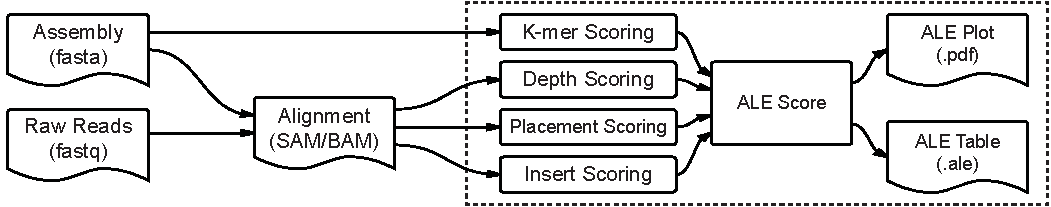
\includegraphics[width=\textwidth]{figures/ALE/Clark_Fig1c.pdf}}
    \caption[Components of the ALE score]{The components of the total ALE score. ALE takes a proposed assembly and an alignment of reads as input. Four scores, the k-mer, placement, depth and insert sub-scores are computed using the model described in the Methods section. From the four scores a total ALE score is calculated and reported as a text file (.ale), and the text file can be used for input into the supplied plotter to generate a PDF file for visualization.}\label{fig:01}
\end{figure*}

Figure 1 shows the pipeline used to compute the total ALE score. Given a set of reads and a proposed assembly, ALE first takes as input the alignments of the reads onto the assembly in the form of a SAM or BAM file \cite{Li2009}, which can be produced by a third-party alignment algorithm such as bowtie \cite{Langmead2009} or bwa \cite{Li2009}. ALE then determines the probabilistic placement of each read and a corresponding placement sub-score for each mapped base, which describes how well the read agrees with the assembly.  In the case of paired end reads, ALE also calculates an insert sub-score for all mapped bases of the assembly from the read pair, which describes how well the distance between the mapped reads matches the distribution of lengths that we would expect from the library.  ALE also calculates a depth sub-score, which describes the quality of the sequencing depth accounting for the GC bias prevalent in some NGS technologies.  The placement, insert and depth scores together determine $P(R|S)$.  Independently, with only the assembly and not the reads, ALE calculates the k-mer sub-score and $P(S)$. Each sub-score is calculated for each scaffold or contig within an assembly independently, allowing for variations commonly found in metagenomes. The four sub-scores are then combined to form the total ALE score. The constituent calculations in this pipeline are described in the Methods section \ref{sec:ingredients_of_ALE_score} and \ref{sec:ApproxZ}.

In addition, these four sub-scores are reported by ALE as a function of position within the assembly, and can be visualized with the included plotting package or imported in table form to another package such as the Integrative Genomics Viewer (IGV) \cite{Nicol2009}, or the UCSC genome browser \cite{Kent2002}.  When used in this way, these sub-scores can be used to locate specific errors in an assembly. 

% section The ALE Score and the likelihood of an assembly (end)

\section{Probabilistic ingredients of the total ALE score} % (fold)
\label{sec:ingredients_of_ALE_score}

We can combine the two probabilities, $P(R|S)$ and $P(S)$, to provide an expression for the probability of the assembly given the reads, $P(S|R)$.  While this combined expression is too computationally expensive to compute exactly because of the normalization factor, ALE provides a summary measure of quality called the total ALE score that is proportional to $P(S|R)$ and can be used compare assemblies.

Below, we first describe how $P(R|S)$ and $P(S)$ are computed from a set of reads $R$ and a given assembly $S$.  We then describe how they are combined to compute the ALE score, and how the ALE score can be used to compare the qualities of different assemblies. We first provide an overview of how $P(R|S)$ and $P(S)$ are defined and computed, beginning with $P(R|S)$ and then discussing $P(S)$.

The statistical model from which $P(R|S)$ is calculated supposes that each paired read is generated at random from the genome or collection of genomes according to the following process.  First, the distance between the two paired read ends, and their orientation, is chosen at random from a distribution that is specific to the library used to generate them.  Second, the locations of the mate pairs on that genome are chosen at random, potentially with a consistent GC bias.  Third and finally, the content of each of the two paired ends are generated by taking the genome's true base pairs at the chosen locations and then copying these base pairs into the reported read, with a given probability of error, insertion, or deletion for each base pair given by the sequencer's quality score.

The likelihood $P(R|S)$ that results from this process can be factored into three components
\begin{equation}
    P(R|S)=P_{\text{placement}}(R|S)P_{\text{insert}}(R|S)P_{\text{depth}}(R|S).
\end{equation}

The first component, $P_{\text{placement}}(R|S)$ describes how well the reads' contents match the assembly at the locations to which they are mapped. The second component, $P_{\text{insert}}(R|S)$, describes how well the distances and orientations between each paired read match the distances and orientations that we would expect from the library.  The third component $P_{\text{depth}}(R|S)$ describes how well the depth at each location agrees with the depth that we would expect given the GC content at that location. Contributions to these three quantities, as a function of position in the assembly, are used to produce the placement, insert and depth sub-scores.

Together with the likelihood of the reads $R$ given the assembly $S$, $P(R|S)$, the ALE framework also depends upon a Bayesian prior probability distribution over assemblies, written $P(S)$.  $P(S)$ describes how likely we would believe the assembly $S$ to be, if we did not have any read information.  In this prior probability distribution, we encode the belief that within a single genome, each k-mer has a unique k-mer frequency. This is the frequency of any set of k base pairs appearing in order in the genome. This defines a $4^{k}$ dimensional vector that is conserved across a genome and can help discover when different genomes have been mistakenly combined in a metagenome setting \cite{Teeling2004} \cite{Woyke2006}. Because $P(S)$ is determined by k-mer frequencies, we use the notation $P_{\text{kmer}}(S)$ rather than the more generic $P(S)$ when referring to this probability distribution. Contributions to $P_{\text{kmer}}(S)$ as a function of position in the genome is referred to as the k-mer sub-score.

\subsection{Placement sub-score} % (fold)
\label{sub:Placement sub-score}

$P_{\text{placement}}(R|S)$ quantifies the likelihood of observing a read $r_{i}$, or set of reads $R$, given an assembly $S$. It includes information about how the read maps onto the assembly, the quality score of each base and orientation.

We assume that every paired read is independent of all other pairs of reads, which allows us to write $P_{\text{placement}}(R|S)$ as
\begin{equation}
    P_{\text{placement}}(R|S) = \prod_{r_{i} \in R} P_{\text{placement}}\left(r_{i}|S\right),
\end{equation}
where $P_{\text{placement}}\left(r_{i}|S\right)$ describes how well the contents of a single read $r_{i}$ match the assembly at the locations to which they are mapped, as well as how well the distance and orientation between that read's paired ends match the distance and orientation that we expect from the library.  We assume independence of these distributions, allowing us to write this as
\begin{equation}
    P_{\text{placement}}\left(r_{i}|S\right) = P_{\text{matches}}\left(r_{i}|S\right)P_{\text{orientation}}\left(r_{i}|S\right). 
\end{equation}
$P_{\text{matches}}\left(r_{i}|S\right)$ measures how well the read matches the section of the assembly to which it maps. Making the assumption that each base $j$ of the read is correctly called by the sequencer independently with a probability equal to the base's quality score $Q_{j}$, we can write this as
\begin{equation}
    P_{\text{matches}}\left(r_{i}|S\right) = \prod_{{\rm base}_{j} \in r_{i}} P\left({\rm base}_{j}|S\right)
\end{equation}
where
\begin{equation}
    P\left({\rm base}_{j}|S\right) = Q_{j}
\end{equation}
when the base $j$ correctly matches the assembly and
\begin{equation}
    P\left({\rm base}_{j}|S\right) = (1-Q_{j})/4
\end{equation}
when it does not. This expression follows from our modeling assumption that all 4 possible errors that the sequencer could have reported at that base (three different substitutions and a deletion) are equally likely when the read does not match the sequence. This symmetry requires each of the four possible reported errors (a base not equal to the assembly or a deletion) to have equal probability. An insertion, which does not have a corresponding base in the assembly, is modeled similarly, with the 4 in the denominator representing the uniform likelihood of observing any of the 4 possible bases on the assembly at that position. The product across all bases in a read is then equal to the total probability of observing that particular read at the given location in the assembly.

If the assembly has an unknown base at the location (denoted by an ``N") then we set
\begin{equation}
    P\left({\rm base}_{j}|S\right) = 1/4
\end{equation}
modeling the fact that there is no information about the correct base at that location with a uniform distribution over all 4 possible bases. If an ambiguity code is reported by the sequencer then the above expression is modified to account for a distribution over the possible bases encoded by the corresponding code (see Table \ref{ambcodes}).

Each read is only allowed to be ``placed" at a single position in the assembly. If the aligner placed a particular read at more than one position, we choose a single position at random, weighted by $P_{\text{placement}}(r_{j}|S)$ score for each proposed position of the read on the assembly. This allows for repeat regions to be properly represented with the correct number of reads in expectation.

The orientation likelihood, $P_{\text{orientation}}\left(r_{i}|S\right)$, is calculated by first counting the number of times that each orientation occurs in the library using the mapping information.  The probability that a particular read from a particular library has a particular orientation is then modeled as that orientation's empirical frequency in the library (this can be overridden with user-specified values for the probabilities).  The likelihood $P_{\text{orientation}}\left(r_{i}|S\right)$ is then the empirical frequency of the observed orientation of the read $r_{i}$ in the library from which $r_{i}$ belongs.

After combining these two independent probabilities we are left with the total placement score $P_{\text{placement}}(R|S)$ for a given read.  Below, we use this when calculating the probability that an assembly is correct given the reads, as well as the overall total ALE score.  We also use it to calculate per-base placement scores at particular positions in the assembly.  The placement sub-score at a particular position is given as the geometric mean of $P(r_{j}|S)$ of all $r_{j}$ covering that specific position,
\begin{equation}
    \left[\prod_{R^{\prime}}P(R|S)\right]^{1/N}
\end{equation}
where the product is over all reads $R^{\prime}$ covering the given position, and $N$ is the number of such reads.

% subsection Placement sub-score (end)

\subsection{Insert sub-score} % (fold)
\label{sub:Insert sub-score}

The insert likelihood, $P_{\text{insert}}\left(r_{i}|S\right)$, is determined by first observing all insert lengths from all mappings of all reads and calculating the population mean, $\mu$, and standard deviation, $\sigma^{2}$ of these lengths (the mean and standard deviation can also be set by the user, if they are known). This step only needs to be done once.  Once completed, we calculate the insert likelihood for each read $r_{i}$ by assuming that the corresponding observed insert length $L_{i}$ is distributed normally with this mean and variance, so that
\begin{equation}
    P_{\text{insert}}\left(r_{i}|S\right) = {\rm Normal}\left(L_{i};\mu,\sigma^{2}\right).
\end{equation}
In this expression, the insert length $L_{i}$ is computed from the read $r_{i}$ and its mapping to the assembly $S$. Similar to the placement score we can calculate the geometric mean of insert scores at a given position to come up with the insert sub-score. This can be useful for determining areas of potential constriction or expansion within a proposed assembly.

% subsection Insert sub-score (end)

\subsection{Depth sub-score} % (fold)
\label{sub:Depth sub-score}

$P_{\text{depth}}(R|S)$ describes how well the depth at each location agrees with the depth that we would expect given the GC content at that location (which is ideally Poisson-distributed \cite{Lander1988}).

For each read, the GC content is the proportion of bases that are either G or C. Modern sequencers and library preparation techniques can bias GC-rich areas of a genome \cite{Aird2011} This bias affects the observed depth of reads mapping onto specific areas of an assembly. To correct for this bias we first calculate for each of the following 100 ranges of GC content over the average read length, 0\% to 1\%, 1\% to 2\%, $\ldots$, 99\% to 100\%, the average observed depth for positions in each contig in the assembly with a GC content in this range. Call $\mu_{\text{depth}(X_{i})}$ the observed average depth of all reads with a GC content falling in the same range as the GC content percentage $X_{i}$. We set the minimum expected depth to be 10, discounting regions of exceptionally low average depth.

We model the depths to be Poisson distributed about a mean drawn from a Gamma distribution centered at the expected depth for that position given its GC content. This models the dependence of the expected depth on more than just the GC content at that position, such as the presence of ``hard stops" (regions with no reads mapping to them) and the GC content at nearby positions. It results in an infinite mixture of Poissons that is equivalent to a Negative Binomial distribution. For simplicity and computational convenience, we make an independence assumption when computing this component.  This causes the expected coverage at a location to depend only upon the GC content at that position, and not the GC content at nearby positions.

Then, at any given position the depth sub-score is
\begin{equation}
    \begin{array}{l}
        P_{\text{depth}}\left(d_{j}|S,X_{i}\right) \\
        = {\rm Poisson}\left(d_{j};Y_{i}\right), Y_{i} \sim {\rm Gamma}(\max(10,\mu_{\text{depth}(X_{i})}), 1) \\
        = {\rm NegBinom}(d_{j}; \max(10, \mu_{\text{depth}(X_{i})}), 1/2)
    \end{array}
\end{equation}
where the depth is $d_{i}$ and where the GC content percentage $X_{i}$ is averaged across all reads that map (in the placement step) to that position. See Section \ref{sec:GCBias} for a further analysis.

% subsection Depth sub-score (end)

\subsection{k-mer sub-score} % (fold)
\label{sub:kmersubscore}

$P_{\text{kmer}}(S) \propto P(S)$, the k-mer sub-score, describes the likelihood of the assembly $S$, in the absence of any read information.  Within this prior probability distribution, we encode the belief that within a single genome, each k-mer (a permutation of $k$ base pairs, where k is a fixed user defined number initially set to 4) has a unique k-mer frequency. This is the frequency with which the k-mer appears in the genome.  The $4^{k}$ dimensional vector giving this frequency for each k-mer is conserved across a genome and can help determine if two different genomes have been mistakenly combined \cite{Teeling2004} \cite{Woyke2006}. Let $K$ be the set of all possible unique k-mers, so $|K| = 4^{k}$, and for each $i$ in $K$ let $n_{i}$ be the number of times this k-mer appears in a contig in the assembly. Then, the frequency $f_{i}$ of a particular k-mer $i$ within a contig is
\begin{equation}
    f_{i} = \frac{n_{i}}{\sum_{j\in K}n_{j}}.
\end{equation}
The k-mer score is the product of this frequency over each k-mer appearing in each contig of the assembly $S$, which can be written as
\begin{equation}
    P_{\text{kmer}}(S) = \prod_{i\in K} f_{i}^{n_{i}}.
\end{equation}
This is equivalent to assuming each k-mer in the assembly is drawn independently with identical distributions from a multinomial distribution with probabilities empirically estimated from the assembly.

The k-mer sub-score of a base at any given position in the assembly is the (geometric) average of $P_{\text{kmer}}(S)$ of all k-mers that cover that position. In calculating this average, the very first base in the genome only has one contributing k-mer, the second has two, up to k contributing k-mers after $k-1$ bases.

% subsection k-mer sub-score (end)

% section Probabilistic ingredients of the total ALE score (end)

\section{Approximating Z} % (fold)
\label{sec:ApproxZ}

Bayes' rule tells us that the probability that the assembly $S$ is correct is
\begin{equation}
    P(S|R) = \frac{P(R|S)P(S)}{Z}
\end{equation}
where $Z$ is a proportionality constant that ensures that $P(S|R)$ is a probability distribution, where $Z$ is found by summing over all possible assemblies $S^{\prime}$,
\begin{equation}
    Z = \sum_{S^{\prime}}P(R|S^{\prime})P(S^{\prime}).
\end{equation}
$Z$ cannot be explicitly computed because the space of all possible assemblies is far too large ($4^{L}$ where $L$ is the length of the assembly). 

Instead we compute an approximation $\hat{Z}$ to $Z$.  This provides an approximation to $P(S|R)$,
\begin{equation}
    P(S|R) \approx \frac{P(R|S)P(S)}{\hat{Z}}.
\end{equation}

We can compare two assemblies generated from the same library of reads without calculating $Z$, the denominator in our Bayesian likelihood framework, because it cancels when taking the ratio of the likelihoods of the two assemblies. To determine a total ALE score for a single assembly, however, we must calculate or approximate $Z$. Our goal in approximating $Z$ is to use a quantity that does not depend on the assembly $S$ (or only depends weakly through some empirically estimated quantities included as parameters in the overarching statistical model), and is approximately of the same order of magnitude as the exact value of $Z$.  In this section, we refer to our approximate $Z$ as $\hat{Z}$, and define it as a product of the terms,
\begin{equation}
    \hat{Z} = \hat{Z}_{\text{placement}}\hat{Z}_{\text{insert}}\hat{Z}_{\text{depth}}\hat{Z}_{\text{kmer}}.
\end{equation}
We will define each term in this product separately.

\subsection{Approximating arbitrary $Z$}
\label{arbZ}

The $Z$ normalization factor in Bayes' Theorem is defined as
\begin{equation}
    Z = \sum_{S^{\prime}}P(R|S^{\prime})P(S^{\prime}).
\end{equation}
The problem with computing this value explicitly is 
\begin{enumerate}
    \item The space $S^{\prime}$ is very large ($4^{L}$ where $L$ is the length of an assembly).
    \item The set of assemblies for which $P(R|S^{\prime})$ is above a certain threshold $\epsilon > 0$ (like floating point precision $\epsilon = 10^{-8}$) is very small compared to the entire space. This is because the probability $P(R|S^{\prime})$ falls off very quickly when the reads do not agree with the assembly $S^{\prime}$, but this is still too large of a space to compute $Z$ explicitly.
\end{enumerate}

If we make the approximation
\begin{equation}
    P(R|S^{\prime}) \approx \mathbb{E}_{}\left[P({\bf R}|S^{\prime})\right] = \sum_{r \in R^{\prime}} P(r|S^{\prime})P(r|S^{\prime}) = \sum_{r \in R^{\prime}} P(r|S_{0})^{2},
\end{equation}
where $R^{\prime}$ is the set of all possible reads and ${\bf R}$ is a random set of reads drawn from this set and $S_{0}$ is an arbitrary assembly. We drop the dependence on $S^{\prime}$ in the final equality because when summing over all possible reads every combination of read and assembly is evaluated, regardless of the specific assembly compared against. This is to say that for any fixed $S$, every possible permutation of reads (location and number of errors, quality scores, insert lengths, orientations, depths) is evaluated with respect to that assembly. Let $E$ be the set of all possible errors between a read and an assembly and all combinations thereof, (for example, substitution error at position 9 with quality score .97, etc). Then
\begin{equation}
    \mathbb{E}_{}\left[P(R|S^{\prime})\right] = \sum_{r \in R^{\prime}} P(r|S^{\prime})^{2} = \sum_{E} \sum_{r_{e} \in R_{e}^{\prime}} P(r_{e}|S^{\prime})^{2} = \sum_{r \in R^{\prime}} P(r|S_{0})^{2},
\end{equation}
where $R_{e}^{\prime}$ is the set of reads containing the errors $e \in E$. $E$ contains all possible errors (including no errors) so the space of reads can be partitioned with respect to the errors when compared to any fixed assembly $S^{\prime}$. The value of $P(r_{e}|S^{\prime})$ is fixed by the model and independent of the assembly. If there is an error at a specific position, the placement score depends on the type of error and the quality score of the read at that position, which is encoded in $e \in E$. So we can set $P(r_{e}|S^{\prime}) = A_{e}$ where $A_{e}$ is a value independent of $S^{\prime}$.

In fact, this is true for any such assembly, making the dependence on $S^{\prime}$ moot. Our equation for $Z$ then becomes
\begin{equation}
    Z \approx \sum_{S^{\prime}} \mathbb{E}_{}\left[P(R|S^{\prime})\right] P(S^{\prime}) = \sum_{S^{\prime}} \left[\sum_{r \in R^{\prime}} P(r|S_{0})^{2}\right] P(S^{\prime}) = \sum_{r \in R^{\prime}} P(r|S_{0})^{2} = \hat{Z}
\end{equation}
because $\sum_{S^{\prime}}P(S^{\prime}) = 1$ and the dependence on $S^{\prime}$ is dropped.


\subsection{Approximating $Z_{\text{placement}}$} % (fold)
\label{sub:Aprroximating Z_placement}

$\hat{Z}_{\text{placement}}$ is defined as
\begin{equation}
    \hat{Z}_{\text{placement}} = \prod_{r \in R} \hat{Z}_{\text{placement}}(r|S).
\end{equation}
In this expression $R$ is the set of reads actually observed, $r$ is one read in this set of reads, and $\hat{Z}_{\text{placement}}(r|S)$ is defined as
\begin{equation}
    \begin{array}{lcl}
        \hat{Z}_{\text{placement}}(r|S) & = & \mathbb{E}\left[P_{\text{placement}}\left({\bf r^{\prime}}\right)|S\right] \\
        & = & \sum_{r^{\prime} \in R^{\prime}} \left[ P_{\text{placement}}(r^{\prime}|S)\right]^{2} \\
        & = & \sum_{\text{matches}} \sum_{\text{orientation}} \left(P_{\text{matches}}(r^{\prime}|S)P_{\text{orientation}}(r^{\prime}|S)\right)^{2}
    \end{array}.
\end{equation}
In this expression $R^{\prime}$ is the set of all possible reads of the length given by $r$ and ${\bf r^{\prime}}$ is a random set of reads drawn from that set. We sum over all possible matches and orientations, which is analogous to summing over all possible reads. Although $S$ appears in this expression, its value does not depend on $S$ because of permutation symmetry as described in Section \ref{arbZ}. This symmetry allows us to calculate this expression analytically, without enumerating over $R^{\prime}$.  In addition to its lack of dependence of $S$ and its ease of computation, this choice for $P_{\text{placement}}(r)$ is motivated by the belief that this quantity scales roughly like
\begin{equation}
    P_{\text{placement}}(r) = \sum_{S^{\prime}}P_{\text{placement}}(r|S^{\prime})P(S^{\prime}),
\end{equation}
which is a quantity identical in form to $Z$, but restricted to the placement probability of a particular read.

% subsection Approximating $Z_{\text{placement}}$ (end)

\subsection{Approximating $Z_{\text{insert}}$} % (fold)
\label{sub:Aprroximating Z_insert}

We define $\hat{Z}_{\text{placement}}(r|S)$ as,
\begin{equation}
    \begin{array}{lcl}
        \hat{Z}_{\text{placement}}(r|S) & = & \mathbb{E}\left[P_{\text{insert}}\left(r^{\prime}\right)|S\right] \\
        & = & \sum_{r^{\prime} \in R^{\prime}} \left[ P_{\text{insert}}(r^{\prime}|S)\right]^{2} \\
        & = & \sum_{\text{insert}} \left(P_{\text{insert}}(r^{\prime}|S)\right)^{2}
    \end{array},
\end{equation}
where again, in this expression $R^{\prime}$ is the set of all possible reads of the length given by $r$ and ${\bf r^{\prime}}$ is a random set of reads drawn from that set. Similarly, we sum over all possible insert lengths.

% subsection Approximating $Z_{\text{insert}}$ (end)

\subsection{Approximating $Z_{\text{depth}}$} % (fold)
\label{sub:Aprroximating Z_depth}

We define $\hat{Z}_{\text{depth}}$ as,
\begin{equation}
    \hat{Z}_{\text{depth}} = \prod_{{\rm base}_{i} \in S} \hat{Z}_{\text{depth}} \left(X_{i}|S\right),
\end{equation}
where
\begin{equation}
    \hat{Z}_{\text{depth}} \left(X_{i}|S\right) = \mathbb{E}\left[P_{\text{depth}} \left({\bf X_{i}}|S\right)|S\right] = \sum_{d=0}^{\infty} \left(P_{\text{depth}}\left(d | X_{i}, S\right)\right)^{2},
\end{equation}
where $P_{\text{depth}}$ is defined as before and ${\bf X_{i}}$ is a random set of depths drawn from the set of possible depths at location $i$. Although $S$ appears in this expression, its value does not depend on $S$. We can calculate this expression analytically using a hyper-geometric function; see implementation section \ref{sec:DepthZnormalization}.

% subsection Aprroximating $Z_{\text{depth}}$ (end)

\subsection{Approximating $Z_{\text{kmer}}$} % (fold)
\label{sub:Aprroximating Z_kmer}

We define $\hat{Z}_{\text{kmer}}$ as the expected kmer score,
\begin{equation}
    \hat{Z}_{\text{kmer}} = \mathbb{E}\left[P_{\text{kmer}}({\bf S})\right] = \left(\sum_{i\in K} f_{i}^{2}\right)^{N},
\end{equation}
where $f_{i}$, $K$ and $n_{i}$ are defined as before in section \ref{sub:kmersubscore} and ${\bf S}$ is a random assembly drawn from the set of all possible assemblies. This method finds the expected k-mer score for a uniform random k-mer and applies that score $N$ times. Although $\hat{Z}_{\text{kmer}}$ depends on $S$ through the empirically determined $f_{i}$, which may be undesirable, this dependence follows naturally from our statistical model because the $f_{i}$ are considered parameters, which are estimated from data and then treated as known by the model. 

% subsection Aprroximating $Z_{\text{kmer}}$ (end)

The preceding calculations allow us to approximate $Z$ and find an ``absolute" likelihood score for a given assembly without comparing it to another assembly with the same library and alignment.

% section Approximating Z (end)

\section{Relationship of the difference of total ALE scores to probability of correctness} % (fold)
\label{sec:Relationship of the difference of total ALE scores to probability of correctness}

Here we derive an expression described in the Results section for the difference of two total ALE scores in terms of the probability that an assembly is correct.  Suppose we have two assemblies, $S_{1}$ and $S_{2}$.  Call $A_{1}$ the total ALE score of the first assembly, and $A_{2}$ the total ALE score of the second assembly, both generated from the same set of reads $R$. The difference of these scores is then
\begin{equation}
    \begin{array}{l}
        A_{1} - A_{2} \\
        = \log\left(P\left(R|S_{1}\right)\right) + \log\left(P\left(S_{1}\right)\right) - \log\left(\hat{Z}\right) + \log\left(P\left(R|S_{2}\right)\right) + \log\left(P\left(S_{2}\right)\right) + \log\left(\hat{Z}\right) \\
        \approx \log\left(P\left(R|S_{1}\right)\right) + \log\left(P\left(S_{1}\right)\right) - \log\left(Z\right) + \log\left(P\left(R|S_{2}\right)\right) + \log\left(P\left(S_{2}\right)\right) + \log\left(Z\right) \\
        = \log\left(\frac{P\left(R|S_{1}\right)P\left(S_{1}\right)}{P\left(R|S_{2}\right)P\left(S_{2}\right)}\right)
    \end{array}.
\end{equation}

% section Relationship of the difference of total ALE scores to probability of correctness (end)

\section{Correction for GC Bias} % (fold)
\label{sec:GCBias}

Modern sequencers have a GC bias, which is to say that regions of the genome with different concentrations of the bases {\bf G} and {\bf C} will produce different numbers of reads, which will lead to the coverage of these regions within an assembly to vary. In Figure \ref{fig:GC1} we see the average depth at different GC concentrations within a {\it Spirochaeta smaragdinae} genome with reads generated from an Illumina sequencer. This variation in average depth can cause many false positives related to the ALE depth score. The Poisson distribution drops off steeply, which is to say that depth values away from the global mean would be scored very low, due solely to the inherent depth bias of the sequencer. We need to model this bias to eliminate these false positives.

\begin{figure}[!tpb]%figure1
    \centerline{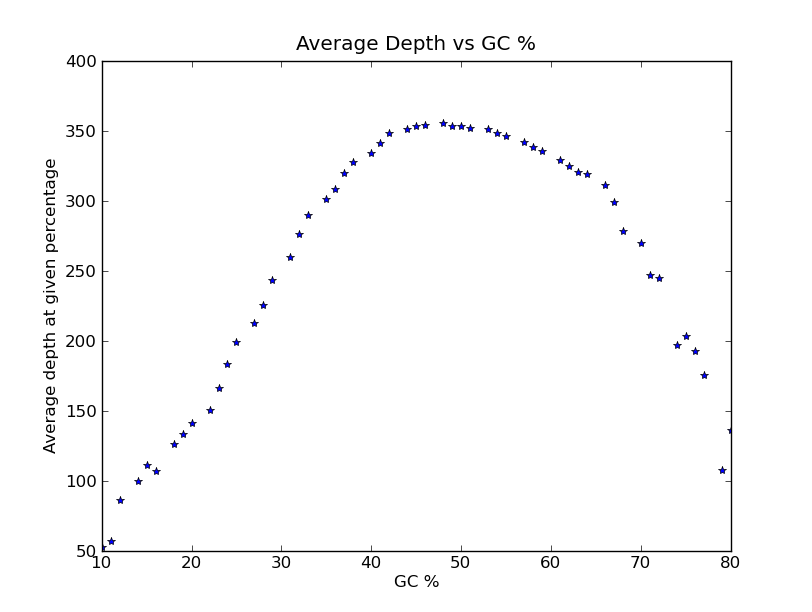
\includegraphics[width=\textwidth]{figures/ALE/avgDepthVsGC.png}}
    \caption[Average depth vs. GC content]{The average depth at various GC contents in the {\it Spirochaeta smaragdinae} genome for reads of length $l = 77$.}\label{fig:GC1}
\end{figure}

We define the average GC content of a base relative to a read length $l$ as the average GC content of all reads of length $l$ that could possibly overlap that position.

Assume we look at the following subsequence, focusing on the G at position 4 and assuming that the reads are of length 4.

\singlespacing
\begin{center}
\texttt{...1234567...\\
...ATCGTCA...}
\end{center}
\normalspacing

One sees the following possible reads of length $l=4$ that can overlap with position 4 with their corresponding GC content (Table \ref{GCcontTable})

\begin{table}[h]
    \label{GCcontTable}
    \caption{GC content of reads}
\begin{center}
\begin{tabular}{c|c}
    read & GC content \\
    \hline
    \texttt{ATCG} & 50\% \\
    \texttt{TCGT} & 50\% \\
    \texttt{CGTC} & 75\% \\
    \texttt{GTCA} & 50\%
\end{tabular}
\end{center}
\end{table}

This implies that the base at position 4 is marked with an effective average GC content of 56.25\% given reads of length $l=4$.

\begin{figure}[hptb]
    \centerline{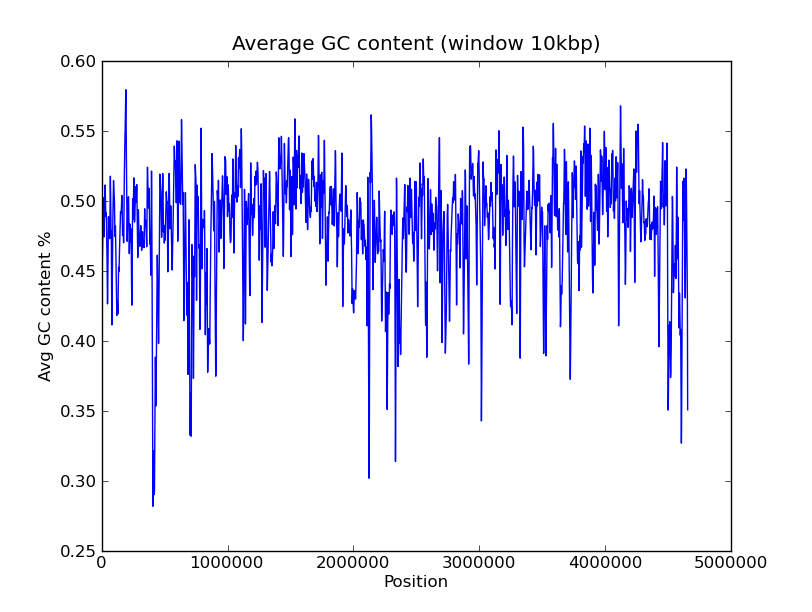
\includegraphics[width=\textwidth]{figures/ALE/spiroGC.png}}
    \caption[GC content of {\it Spirochaeta smaragdinae}]{The GC content can vary greatly within a genome. This figure illustrates the GC content of various positions along the {\it Spirochaeta smaragdinae} genome for read length $l=77$.}\label{fig:GC2}
\end{figure}

\begin{figure}[hptb]
    \centerline{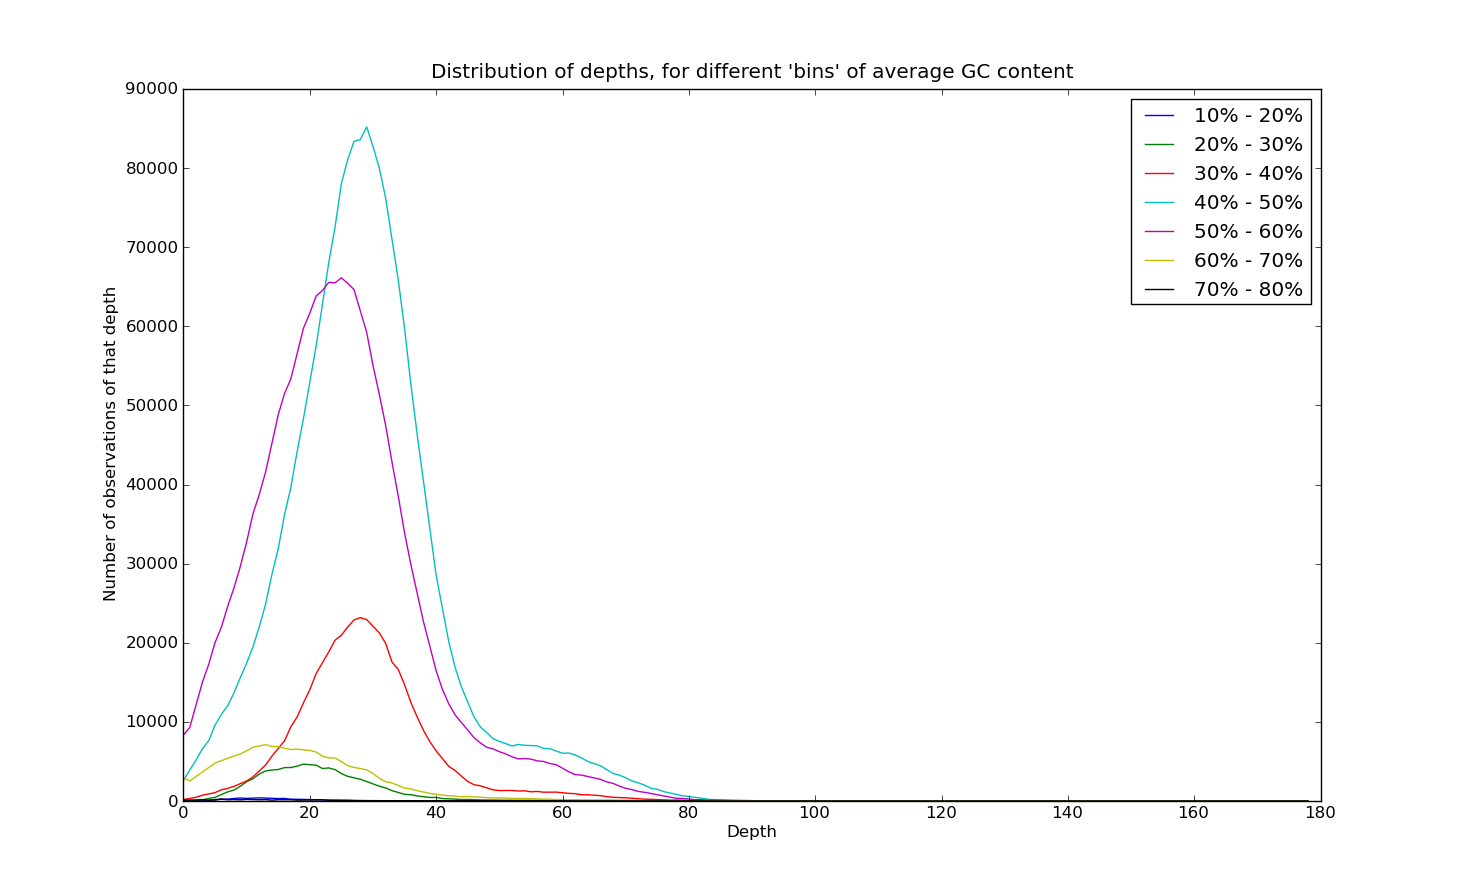
\includegraphics[width=\textwidth]{figures/ALE/DepthDistVsGC_564lib.png}}
    \caption[Depth distribution of different GC contents]{The depth distributions for different ranges of GC content within the {\it Spirochaeta smaragdinae} genome. We can see that the distributions have a fat tail and have varying means.}\label{fig:GC3}
\end{figure}

We can see that the GC bias of the sequencer violates the assumption that the depth is Poisson distributed with a uniform mean. To correct for this bias we model the depth $d$ at a position $j$ being Poisson distributed with a mean drawn from a Gamma distribution related to the depth at that positions GC content,
\begin{equation}
    P_{\text{depth}}\left(d_{j}|S,X_{i}\right) = {\rm Poisson}\left(d_{j};Y_{i}]\right)
\end{equation}
with
\begin{equation}
    Y_{i} \sim {\rm Gamma}(\max(10,\mu_{\text{depth}(X_{i})}), 1).
\end{equation}
We set the mean of the Gamma distribution to the average depth of all positions with the same GC content $\mu_{\text{depth}(X_{i})}$. The minimum value of the parameter is set to 10 in practice to further discount hard stops (positions with 0 depth) and contigs that have very low, but consistent depth, which represents low evidence.

The above equations result in a Negative Binomial distribution,
\begin{equation}
    P_{\text{depth}}\left(d_{j}|S,X_{i}\right) = {\rm NegBinom}(d_{j}; \max(10, \mu_{\text{depth}(X_{i})}), 1/2),
\end{equation}
where the second parameter is analytically equal to $\frac{1}{2}$.

This model has the benefit of incorporating the inherent GC bias of the sequencer and fitting the data well (Figure \ref{fig:GC4}). The ALE depth scores that are generated by using this distribution have a lower variance (see Figure \ref{fig:GC5}). This means that scores that deviate from the mean are not scored as low as when using the Poisson distribution.

\begin{figure}[hptb]
    \centerline{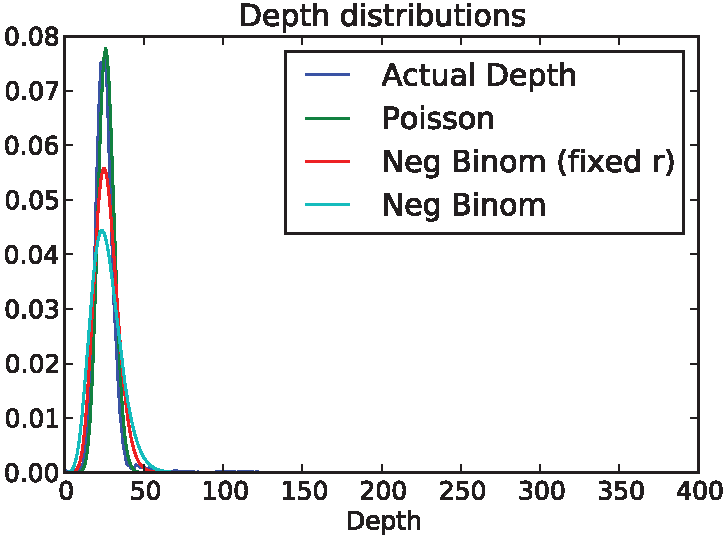
\includegraphics[width=0.5\textwidth]{figures/ALE/GC_depth_distributions.pdf}}
    \caption[Various distributions fit to GC content]{The depth distribution for all positions with GC content between 40-50\%. We compare it to a Poisson distribution as well as the maximum likelihood estimated Negative Binomial distributions with and without fixed parameter $r$.}\label{fig:GC4}
\end{figure}

\begin{figure}[hptb]
    \centerline{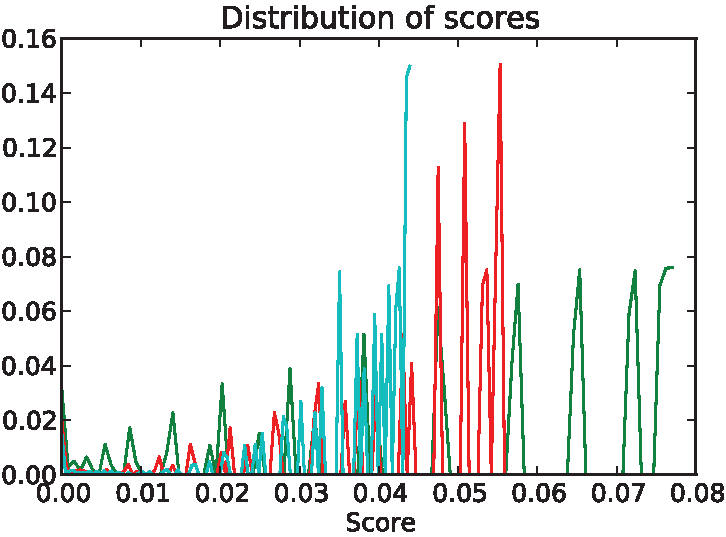
\includegraphics[width=0.5\textwidth]{figures/ALE/GC_depth_distribution_of_scores.pdf}}
    \caption[Distribution of scores using various distributions]{The distributions of ALE depth scores given to positions with 4-=50\% GC content. We see that the Poisson distribution tends to have a fat tail of low scores. This is to say that it is very strict, punishing positions that fall outside of the narrow probability distribution function. The fixed $r$ Negative Binomial function has a large number of medium scores and a low number of very low scores, making it a much more forgiving distribution.}\label{fig:GC5}
\end{figure}

% section Correction for GC Bias (end)

% section Placing reads (end)

\section{Thresholding the total ALE score} % (fold)
\label{sec:Thresholding the total ALE score}

In the plotting program distributed with ALE we use a thresholding algorithm to highlight potential areas of poor assembly quality using the per-base ALE scores. We do this by averaging scores within windows, allowing for the discovery of large errors in the assembly while smoothing out the noise. By the Central Limit Theorem, when we average many independent and identically distributed random variables the result is approximately normally distributed. This allows us to create a ``threshold" for which to delineate ``good" scores from ``bad" and pinpoint problematic regions. This is represented by a solid black line in the figures labeled ``$5\sigma$." This line is calculated by assuming that the individual scores at each position in the assembly are drawn from a mixture of two normal distributions: one for high accuracy and another for low accuracy. We use maximum likelihood to determine the mean and variance of the two underlying distributions. See section \ref{mixturemodel} in the implementation chapter for a more in-depth discussion. The threshold is set as five standard deviations from the mean of the ``high accuracy" distribution. This allows us to readily find areas of inaccuracy that are unlikely to be drawn from an accurate region. Five standard deviations corresponds to 1 false positive in 2 million positions if the joint normal distribution assumptions hold.  The number of standard deviations at which the black line is drawn can be set from the command line by the user.

A black bar is drawn on the plot if the likelihood falls below the threshold at a significant fraction of the positions in any contiguous region with a given length (this fraction and length are user defined, and are initially set to 0.01\% and 1000bp respectively) see figure 3.1, 3.3 and 3.4. The red bars correspond to regions of potential inaccuracy in the assembly that should be examined further. The plotter outputs these regions in a tab delineated text file for easy input into genome viewing software programs like IGV.

% section Thresholding the total ALE score (end)

% chapter ALE Methods (end)

\chapter{ALE Results} % (fold)
\label{cha:ALE Results}

\section{Performance on major types of miss-assemblies in a genome assembly with synthetic data}
Common assembly errors include single-base substitutions, insertion/deletions, chimeric assemblies derived from translocations or misjoins, and copy number errors derived from repeat condensation/expansions. To test ALE's ability to detect these types of errors in an assembly, we generated synthetic reads from a reference genome and then seeded the reference with each type of error. First, 400,000 pair-end synthetic reads were generated from the first 350kbp at random positions of Escherichia Coli K12 Substrain DH10B (\cite{Durfee2008}). Their insert length follows a normal distribution with mean 200bp and standard deviation 7bp. Next, synthetic miss-assemblies were introduced at 6 different locations within this reference.  The miss-assemblies introduced were a substitution, insertion, deletion, inversion, translocation and a copy number error, respectively (Figure \ref{ALEfig2}). We treated this mutated genome as the proposed assembly.

\begin{figure*}[!htpb]%figure1
    \centerline{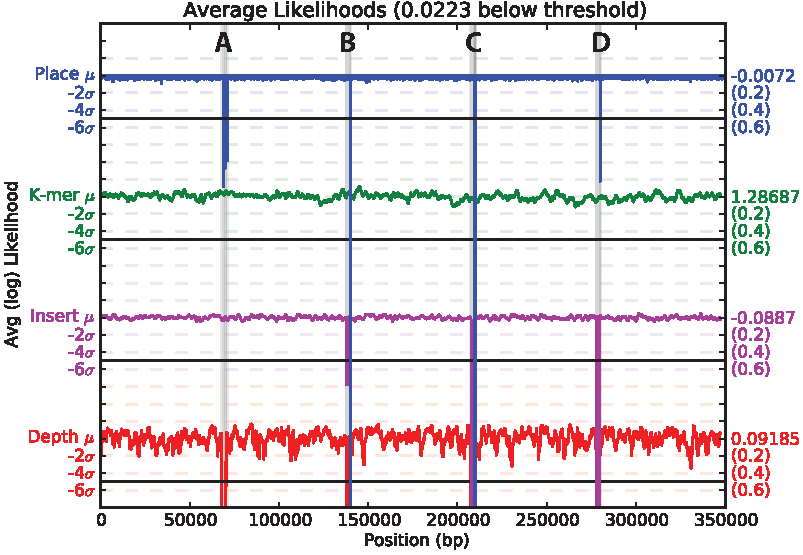
\includegraphics[width=\textwidth]{figures/ALE/fig_2_top.pdf}}
    \caption[ALE performance on with synthetic reads]{The performance of ALE on synthetic errors in {\it E.Coli}. At the genome level, at least one of the four sub-scores drops dramatically in each region containing a synthetic error. A higher resolution view for each type is illustrated in Figure \ref{ALEfig2p1}, \ref{ALEfig2p2}, \ref{ALEfig2p3} and \ref{ALEfig2p4}. ({\bf A}) Substitution, deletion and insertion errors; ({\bf B}) an inversion error; ({\bf C}) an transposition error; and ({\bf D}) an copy number error.}\label{ALEfig2}
\end{figure*}

\begin{figure*}[hptb]%figure1
    \centerline{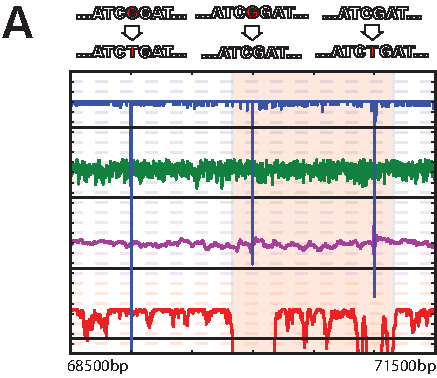
\includegraphics[width=0.6\textwidth]{figures/ALE/fig2_bot_p1.pdf}}
    \caption[ALE performance: synthetic single base errors]{Part {\bf A} of Figure \ref{ALEfig2}: A substitution, deletion and insertion error. The placement sub-score drops significantly at positions 69kbp, 70kbp and 71kbp respectively, which are the locations where the single-base substitution, deletion and insertion errors were added.}\label{ALEfig2p1}
\end{figure*}

\begin{figure*}[hptb]%figure1
    \centerline{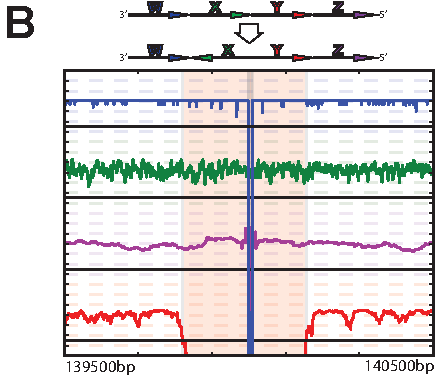
\includegraphics[width=0.6\textwidth]{figures/ALE/fig2_bot_p2.pdf}}
    \caption[ALE performance: synthetic inversion]{Part {\bf B} of Figure \ref{ALEfig2}: An inversion error of length 200bp at position 140kbp causes a drop in the placement, insert and depth sub-score as read mates fail to align to the region.}\label{ALEfig2p2}
\end{figure*}

\begin{figure*}[hptb]%figure1
    \centerline{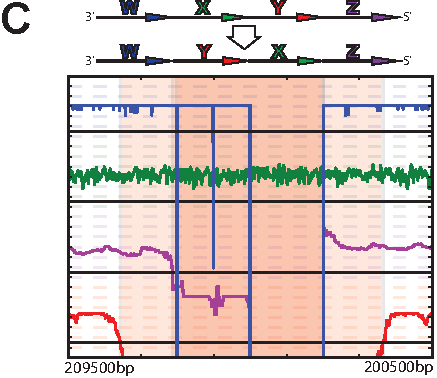
\includegraphics[width=0.6\textwidth]{figures/ALE/fig2_bot_p3.pdf}}
    \caption[ALE performance: synthetic transposition]{Part {\bf C} of Figure \ref{ALEfig2}: A transposition error of length 200bp at position 210kbp and a copy number error of length 77bp at position 280kbp both cause the placement, insert and depth sub-scores to drop.}\label{ALEfig2p3}
\end{figure*}

\begin{figure*}[hptb]%figure1
    \centerline{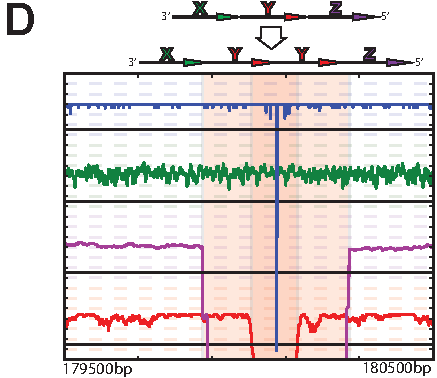
\includegraphics[width=0.6\textwidth]{figures/ALE/fig2_bot_p4.pdf}}
    \caption[ALE performance: synthetic copy number error]{Part {\bf D} of Figure \ref{ALEfig2}: A copy number error of length 77bp (read length) was added at position 280kbp causing the depth and insert scores to drop, as well as the placement at the very center where the two copies meet.}\label{ALEfig2p4}
\end{figure*}

We tested the ALE algorithm by aligning the above synthetic reads to the proposed assembly using bowtie (\cite{Langmead2009}) and ran the results through the ALE software package. ALE automatically thresholds each error (see Methods) and produces plots of the sub-scores near each error using the included plotter (Figure \ref{ALEfig2}). We found that ALE is able to locate each type of error in the proposed assembly. At the genome level, at least one of the four sub-scores drops dramatically in each region containing a synthetic error. With this set of synthetic data, ALE reports no false discoveries. These results suggest that ALE systematically reports all major types of errors with simulated data.

\begin{figure}[!tpb]%figure1
    \centerline{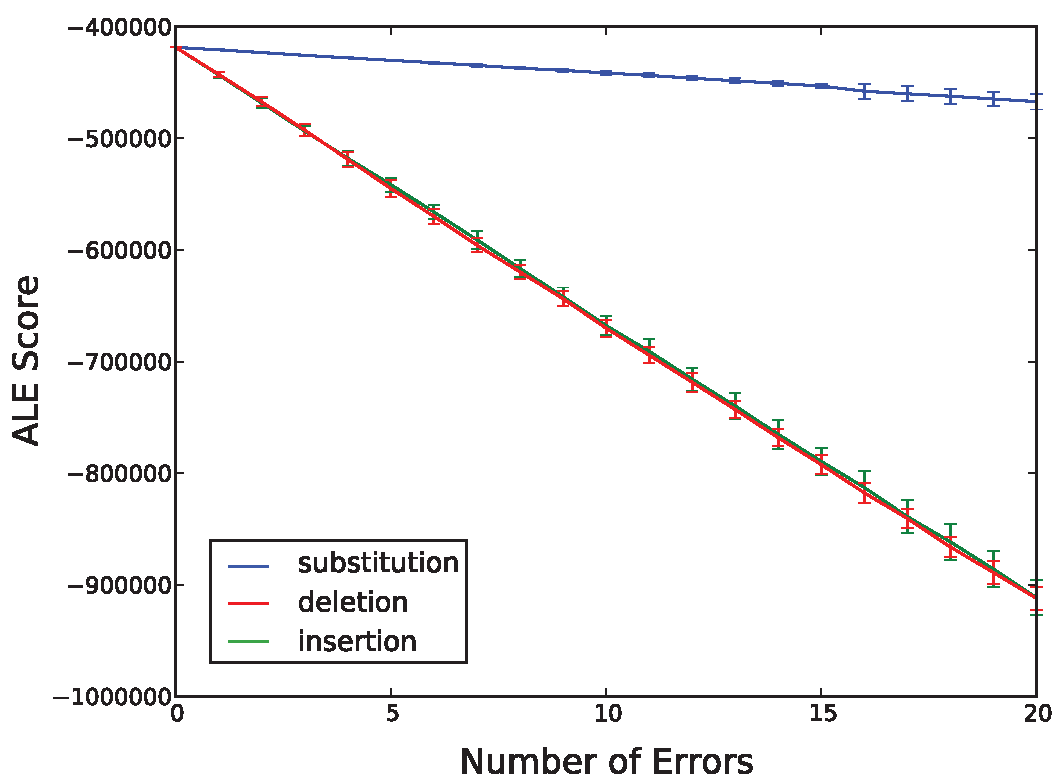
\includegraphics[width=\textwidth]{figures/ALE/Clark_Fig3b.pdf}}
    \caption[ALE score vs. number of errors]{The total ALE score decreases monotonically as the number of errors increases. Insertion (green) and deletion (red) errors cause the total ALE score to drop at a faster rate (per error) than substitution errors (blue) under the model.}\label{ALEfig3}
\end{figure}

Furthermore, the total ALE score decreased as more errors were added to the assembly. As shown in Figure \ref{ALEfig3}, as the number of substitution, insertion and deletion errors increased, the total ALE score decreased monotonically, the rate of which is determined by the quality scores of the data (see Methods section \ref{}). This suggests that the total ALE score indicates overall assembly accuracy.

\section{Detecting chimeric assemblies in a synthetic metagenome}
One common assembly error in metagenome assemblies is the chimeric assembly consisting of two or more genomes. To test ALE's ability to distinguish this type of metagenome-specific error, we simulated a miss-assembled contig by joining several pieces of two genomes (Brachyspira murdochii DSM 12563 (\cite{Pati2010}) and Conexibacter woesei DSM 14684 (\cite{Pukall2010})) in a random order (Figure \ref{ALEfig4}).  Using a known, synthetic reference allows for the unbiased testing of ALE's sensitivity to chimeric metagenomes, since there is not any true metagenome reference available. K-mer sub-scores and plots were generated for this simulated contig as well as the two correct genomes individually for comparison.

\begin{figure*}[!tpb]%figure1
    \centerline{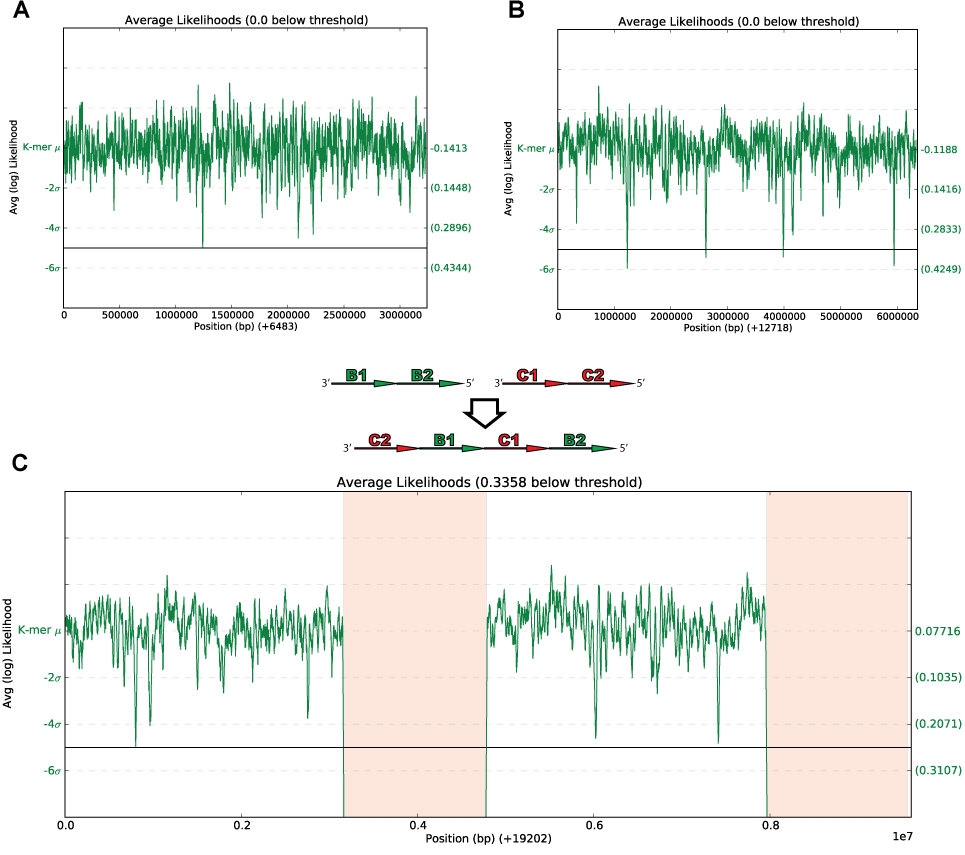
\includegraphics[width=\textwidth]{figures/ALE/Clark_Fig4b.png}}
    \caption[ALE performance on synthetic metagenome]{The performance of ALE on synthetic metagenome assembly errors. ({\bf A} and {\bf B}) The k-mer sub-score for each genome individually. ({\bf C}) k-mer sub-score for a simulated chimeric metagenome between the two genomes. A diagram above ({\bf C}) illustrates how the two genomes were mixed.}\label{ALEfig4}
\end{figure*}

ALE relies on k-mer sub-score (the default is k=4) to distinguish contigs coming from different microbial species, because tetra-nucleotide frequencies are a reliable species-specific signature (\cite{Teeling2004}; \cite{Woyke2006}). If a genome, or contig, contains two or more distinct regions characterized by different k-mer vectors, then the k-mer sub-score will be lower for the positions characterized by the less prevalent k-mer vector (see Methods). Because the other sub-scores are unaffected by the mixture, the drop in total ALE score is due to the lower k-mer sub-score. This unique capability of ALE allows easy detection of chimeric contig/scaffolds within a metagenome assembly. As shown in Figure \ref{ALEfig4}, the k-mer sub-score is consistent for each of the two genomes individually as expected (Figure \ref{ALEfig4}, A and B). In contrast, the k-mer sub-score is much lower for the mixed genomes, clearly identifying where two genomes are mixed together in the same assembly.

\section{Discovery of errors in real genome assemblies}
\label{ALE_res_spiro}

The above experiments used simulated reads, or assemblies with simulated errors. Real reads and real genome/metagenome assemblies are often very noisy, presenting an additional challenge to ALE. To test ALE using real world assemblies with real reads we chose a finished genome, {\it Spirochaeta smargdinae} DSM 11293, originally constructed from 454 and Illumina reads (\cite{Mavromatis2010}), and applied ALE to it using one lane of 2x76 paired end Illumina reads. The results are shown in Figure \ref{ALEfig5} and Table \ref{ALEtab1}. At the genome level, ALE found several errors, including a large 560kbp region (3.91mb – 4.48mp) in the proposed assembly where the depth sub-score dropped below the threshold. We found 3 areas producing errors that are likely due to repeat condensation. For example, further examination of two regions (408kbp-415kbp and 4.241mbp-4.247mbp) by overlaying the Illumina short read data indicates these regions have much higher sequence depth (2X) than neighboring regions, and contain many SNPs (two alleles of roughly equal ratio) (Figure \ref{ALEfig5}, B and C), supporting the hypothesis that there are two copies of these regions in this genome. The boundaries of these regions also have abnormal placement and insert sub-scores, further supporting the hypothesis that there are miss-assemblies at the above locations.

\begin{figure*}[!tpb]%figure1
    \centerline{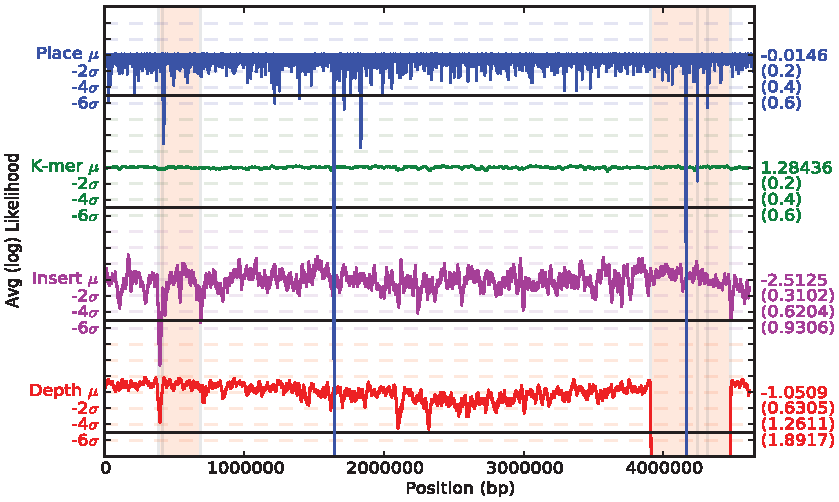
\includegraphics[width=\textwidth]{figures/ALE/fig5_top.pdf}}
    \caption[ALE performance on real reads]{({\bf A}) the ALE plot for {\it Spirochaeta smaragdinae} using 44M paired reads. Four ALE sub-scores were plotted across the entire genome assembly: placement (blue), k-mer (green), insert (purple) and depth (red). miss-assemblies identified by ALE default thresholds were highlighted. Two of these miss-assemblies are displayed in the integrated genome viewer (IGV, in Figure \ref{ALEfig5p2}), with the original Illumina data used by ALE and the validation data from PacBio sequencing. SNPs automatically identified by IGV are shown as colored bars in the sequencing coverage plots (the coverage is indicated by the numbers on the left).}\label{ALEfig5}
\end{figure*}

\begin{figure*}[!tpb]%figure1
    \centerline{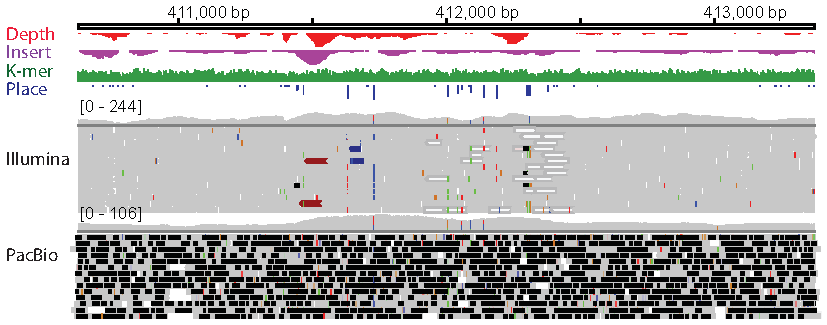
\includegraphics[width=\textwidth]{figures/ALE/fig5_mid.pdf}}
    \centerline{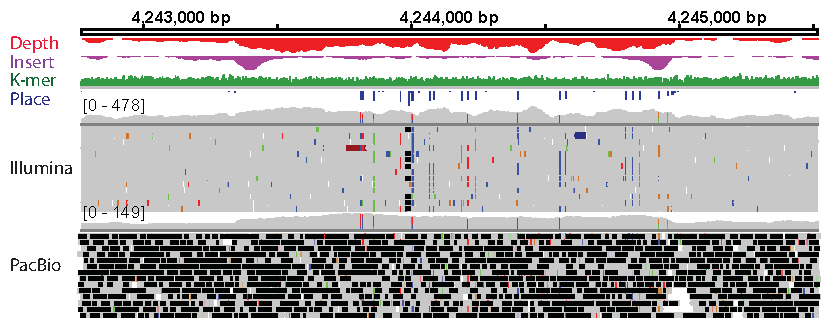
\includegraphics[width=\textwidth]{figures/ALE/fig5_bot.pdf}}
    \caption[ALE real reads: IGV of miss-assemblies]{Two of these miss-assemblies from Figure \ref{ALEfig5} displayed in the integrated genome viewer (IGV), with the original Illumina data used by ALE and the validation data from PacBio sequencing. SNPs automatically identified by IGV are shown as colored bars in the sequencing coverage plots (the coverage is indicated by the numbers on the left).}\label{ALEfig5p2}
\end{figure*}

\begin{table}[!htp]
    \caption{miss-assemblies identified in {\it Spirochaeta smaragdinae}.}
    \label{ALEtab1}
    \begin{center}
%\processtable{miss-assemblies identified in Spirochaeta smaragdinae.\label{Tab:01}}
\begin{tabular}{c|c|c}
Threshold Violation Type & Starting Position & Ending Position\\\hline
Placement & 411624 & 412375\\
Placement & 4243804 & 4244967\\
Placement & 4317554 & 4317856\\
Insert & 383643 & 688112\\
Depth & 3909940 & 4481198\\
\end{tabular}
\end{center}
\end{table}

To determine whether these errors identified by ALE are true assembly errors or Illumina artifacts, we independently validated the results using PacBio sequencing data. A total of 53 SMRT cells comprising 221mb of mapped reads or 34 folds of overage were aligned to the assembly. Manual inspection of the resulting PacBio alignment confirms 5/5 assembly errors (Figure \ref{ALEfig5} B and C \& Table \ref{ALEtab1}), suggesting the errors identified by ALE are true errors in the assembly. 

\section{Sensitivity to SNVs in real data}
\label{SNVsReal}
To show that ALE has a high sensitivity to real errors in real data we examine a re-sequencing project. In this project one lane of Illumina 36x2 paired reads was generated from a new strain of {\it Rhodobacter sphaeroides} 2.4.1 (\cite{Choudhary2006}) with an insert length of ~200bp covering the genome with an average coverage depth of 557. This genome has a very high GC content (68\%) and contains 336 hard stops and many more very low depth regions. A hard stop is a region where a bias in the sequencer causes it to report 0 depth (no reads) without any read pairs spanning the region. This makes SNV detection difficult for many SNP detectors (\cite{Wang2011}). The reads were aligned to the reference genome and used to independently compile a reference set of 222 possible SNVs between the strains (176 from Chromosome1, length 3.2Mbp; 46 from Chromosome2, length 0.94Mbp). The placement sub-score was then computed using the same re-aligned reads.

To determine the positions with the least evidence under the model we sorted the placement sub-scores for each chromosome. The 0.0001\% worst scoring positions (219 regions) on Chromosome1 are within a read length of 154 of the 176 variants (88\%), and the top 0.0005\% worst positions (977 regions) contain more than 97\% of the variants. The same experiment for Chromosome2 recovers 87\% (40 of 46 variants from 63 regions) and 96\% (from 309 regions) respectively. For a further discussion refer to section \ref{ROCALE}. This shows that the positions at which the proposed assembly differs from the genome generating the reads are among the positions with the loewest sub-scores.  The regions with poor sub-scores that do not correspond to the variant list are other regions unsupported by the read evidence, such as hard stops regions of very low coverage that stem from the bias of the sequencer. This shows that ALE can locate regions unsupported by the read evidence, including SNVs, and that ALE accurately gauges assembly quality at multiple base resolutions.

\section{ALE's performance with Pacific Biosciences RS data}
The above experiments were all performed with next generation short read data. Currently, Pacific Biosciences (PacBio) sequencing platform, also referred to as ``third-generation" sequencing, is becoming increasing popular due to its long read length (up to several kb) (\cite{Eid2009}). These long reads are expected to greatly reduce the complexity associated with genome assembly validation. In contrast with the second generation sequencing, single-molecule based PacBio RS sequencing has a much higher base error rate (~15\%), making it an ideal candidate for testing the robustness of ALE against very noisy data. For this purpose we examined the reference genome of {\it Lambda Phage} and corresponding PacBio reads of average depth 548x and a randomly sampled set at 50x. To determine ALE's performance on this dataset, the reference genome was synthetically mutated by adding 12 substitution, insertion and deletion errors at various locations (Table \ref{ALEtab2}). At 548x depth, within the top 12 lowest placement sub-scores, ALE recovered all 12 errors at the mutated positions, while reporting no false positives. At 50x depth, excluding the low coverage edges, the 12 errors were detected in the top 14 lowest placement sub-scores, with 2 false positives.  In comparison, the standard Pacific Biosciences variant caller, EviCons, correctly identified only 10 of these errors with low confidence at default settings and the full 548x depth. This shows that ALE is a robust measure of assembly accuracy with noisy sequencing data, and it is a generic framework that can be used with both short and long sequence read technologies.

\begin{table}[!htp]
        \label{ALEtab2}
    \begin{center}
        \begin{tabular}{cccccc}
Operation & Mutation & Position & 548x& 50x & 548x\\
Type & Details & & Evicon & Rank & Rank\\
 & & & (PacBio) & (ALE) & (ALE)\\
\hline
Sub & C $\rightarrow$ A & 881 & 1 & 5 & 5\\
Ins & CC $\rightarrow$ CCC & 2161 & - & 14 & 12\\
Del & G $\rightarrow$ - & 3681 & 1 & 9 & 8\\
N/A & - & 15712 & - & 7 & -\\
Del & AACGGGCAGA & 16561 & 1 & 4 & 4\\
Ins & AACGGGCAGA & 17030 & 1 & 3 & 2\\
Sub & A $\rightarrow$ G & 22881 & 1 & 10 & 7\\
Sub & T $\rightarrow$ A & 28561 & 1 & 11 & 10\\
Del & T & 34560 & 1 & 12 & 11\\
Sub & G $\rightarrow$ C & 36560 & 1 & 8 & 9\\
Ins & ACGTACGT & 40721 & 1 & 1 & 1\\
N/A & - & 41318 & - & 13 & -\\
Del & TCATCGCG & 43200 & - & 6 & 6\\
Ins & C & 47600 & 1 & 2 & 3
\end{tabular}
\end{center}
\caption[Real Data ALE vs. PacBio]{Performance of ALE on synthetic assembly errors in {\it Lambda Phage} genome with different PacBio sequencing depths (50x and 548x)}
\end{table}

\section{Discussion}

ALE facilitates the rapid discovery of many types of errors in genome assemblies, including metagenomes. It does this by applying a rigorous statistical model and calculating the likelihood of observing a specific assembly given the reads that were used to generate it. This allows ALE to determine specific regions within a proposed assembly that are poorly supported by the reads. By integrating several aspects of the assembly and the reads, including k-mer composition, sequence depth, insert length, and how well individual bases map, ALE is able to find errors as small as a single substitution error or indel, as well as large copy number errors and chimeric metagenome assemblies.

This framework can serve as a guide to optimize the genome assembly in the following two ways. First, total ALE scores can be used to identify the best assembly from those generated by different assembly protocols. Second, by modifying the regions in which ALE reports low sub-scores, more accurate genomes can be constructed. The space of possible corrections to an input genome is too large to allow the current implementation of ALE to be used as an independent assembler, but it could be used to compare and combine the results from different assemblers and produce an assembly that is most likely to be correct. ALE could also be used to present an alternative method for calculating assembly quality in local assembly algorithms such as Genovo (\cite{Laserson2011}).

When used with a reference genome and re-sequencing data, ALE can discover structural variations. As shown in the cases of {\it Spirochaeta smaragdinae} and {\it Rhodobacter sphaeroides}, ALE readily detects structural variations whose sizes vary from a few bases to several hundred kilobases.

ALE is influenced by the quality of its input: the read data and the alignments of those reads onto the proposed assembly. Data with biased content or alignments, while accepted by ALE, tend to produce noisy sub-scores. The robustness of ALE, however, allows for the recovery of an accurate assembly quality measure as long as the random noise is consistent with the statistical model used by ALE (see Methods).

Future experimental work is needed to determine the profile of assembly errors within a given dataset.  This would better characterize the sub-scores of specific assembly errors, and allow the computation of a per-base confidence in the correctness of the assembly at each base from the corresponding sub-scores.  One possible approach would be to select a number of regions with good sub-scores, mutate those regions of the assembly to simulate errors, and then reevaluate the sub-scores at these regions.  Comparing the sub-scores before and after mutation would provide information about the distribution of sub-scores for accurate and erroneous regions, in that dataset.  Additionally, this could inform an auto-correction algorithm based on ALE to fix problematic regions.

In addition, the model could be extended in future work to account for factors like origin of replication bias prevalent in circular genomes, automatic detection of sequencer bias and different potential distributions for insert length and coverage depth. Biases such as hard stops in Illumina could potentially be found by examining unlikely distributions of read orientation at specific locations coupled with low depth. Specific signatures within the different ALE metrics could be used to classify and correct for specific biases, much as ALE currently corrects for GC content (see Methods).

% chapter ALE Results (end)

\chapter{ALE Implementation} % (fold)
\label{cha:ALE Implementation}

\section{Mixture model for score thresholding}
\label{mixturemodel}

In order to distinguish ``good" scores from ``bad" scores in an assembly we make a series of assumptions about the distribution from which the scores are drawn. When we smooth the data we are effectively averaging many random variables corresponding to the scores at a given position, which due to the Central Limit Theorem means that they can be considered to be normally distributed, if they are independent and identically distributed. The independence assumption is made by assuming the length of the assembly is much larger than the length of a read and the fact that reads are considered independent. The scores are all generated from the same model and are therefore identically distributed.

We assume that the scores $\vec{s}$ are drawn from one of two Gaussian distributions, a ``good" distribution $N_{g}$ and a ``bad" distribution $N_{b}$.
\begin{equation}
    p\left(s_{i}|\lambda\right) = w_{g} \phi\left(s_{i} | \mu_{g}, \sigma^{2}_{g}\right) + w_{b} \phi\left(s_{i} | \mu_{b}, \sigma^{2}_{b}\right)
\end{equation}
where $w_{g} + w_{b} = 1$ are weights and $\phi$ is the Normal probability mass function and $\lambda$ is the collection of hyperparameters $\{w_{g}, w_{b}, \mu_{g}, \mu_{b}, \sigma^{2}_{g}, \sigma^{2}_{b}\}$.

The likelihood of the model is
\begin{equation}
    p\left(\vec{s}|\lambda\right) = \prod_{i=1}^{L} p\left(s_{i}|\lambda\right).
\end{equation}
We cannot maximize this likelihood analytically, but we can find local optima using expectation maximization.

\subsection{Expectation maximization}

We iterate using the {\it a posteriori} probability of a single score $s_{i}$ being drawn from one of the two components,
\begin{equation}
    p_{g}(s_{i}, \lambda) = \frac{w_{g} \phi\left(s_{i} | \mu_{g}, \sigma^{2}_{g}\right)}{w_{g} \phi\left(s_{i} | \mu_{g}, \sigma^{2}_{g}\right) + w_{b} \phi\left(s_{i} | \mu_{b}, \sigma^{2}_{b}\right)}
\end{equation}
and
\begin{equation}
    p_{b}(s_{i}, \lambda) = \frac{w_{b} \phi\left(s_{i} | \mu_{b}, \sigma^{2}_{b}\right)}{w_{g} \phi\left(s_{i} | \mu_{g}, \sigma^{2}_{g}\right) + w_{b} \phi\left(s_{i} | \mu_{b}, \sigma^{2}_{b}\right)}
\end{equation}

at each iteration we update the hyperparameters $\lambda$ using the following formulas,
\begin{equation}
    w_{d}^{(t+1)} = \frac{1}{2}\sum_{i=1}^{L} p_{d}(s_{i}, \lambda^{(t)})
\end{equation}
\begin{equation}
    \mu_{d}^{(t+1)} = \frac{\sum_{i=1}^{L} p_{d}(s_{i}, \lambda^{(t)}) s_{i}}{\sum_{i=1}^{L} p_{d}(s_{i}, \lambda^{(t)})}
\end{equation}
\begin{equation}
    \sigma_{d}^{2^{(t+1)}} = \frac{\sum_{i=1}^{L} p_{d}(s_{i}, \lambda^{(t)}) s_{i}^{2}}{\sum_{i=1}^{L} p_{d}(s_{i}, \lambda^{(t)})} - \mu_{d}^{2}
\end{equation}
for each $d \in \{g, b\}$ until the change in the total likelihood is less than some threshold, or after some number of maximum iterations.

To speed up this process only a random 10\% of the data or a random 10,000 points are used to build the model, whichever is smaller. If the model fails to converge, a different random set of data is chosen, up to a maximum number of iterations. This adds a level of robustness that overcomes certain pathological situations where the 2-Gaussian mixture model will fail.

\subsection{Example with ALE depth score}

As an example we will examine the ALE depth score for {\it Spirochaeta smaragdinae} from Section \ref{ALE_res_spiro}. This genome has two distinct regions in the depth score representing ``good" and ``bad" scores. The two Gaussian mixture model fits the data much better than a single Gaussian distribution as seen in Figure \ref{fig:GMM_spiro} and Table \ref{tab:GMM_spiro}.

\begin{figure}[hpt]
 	\centerline{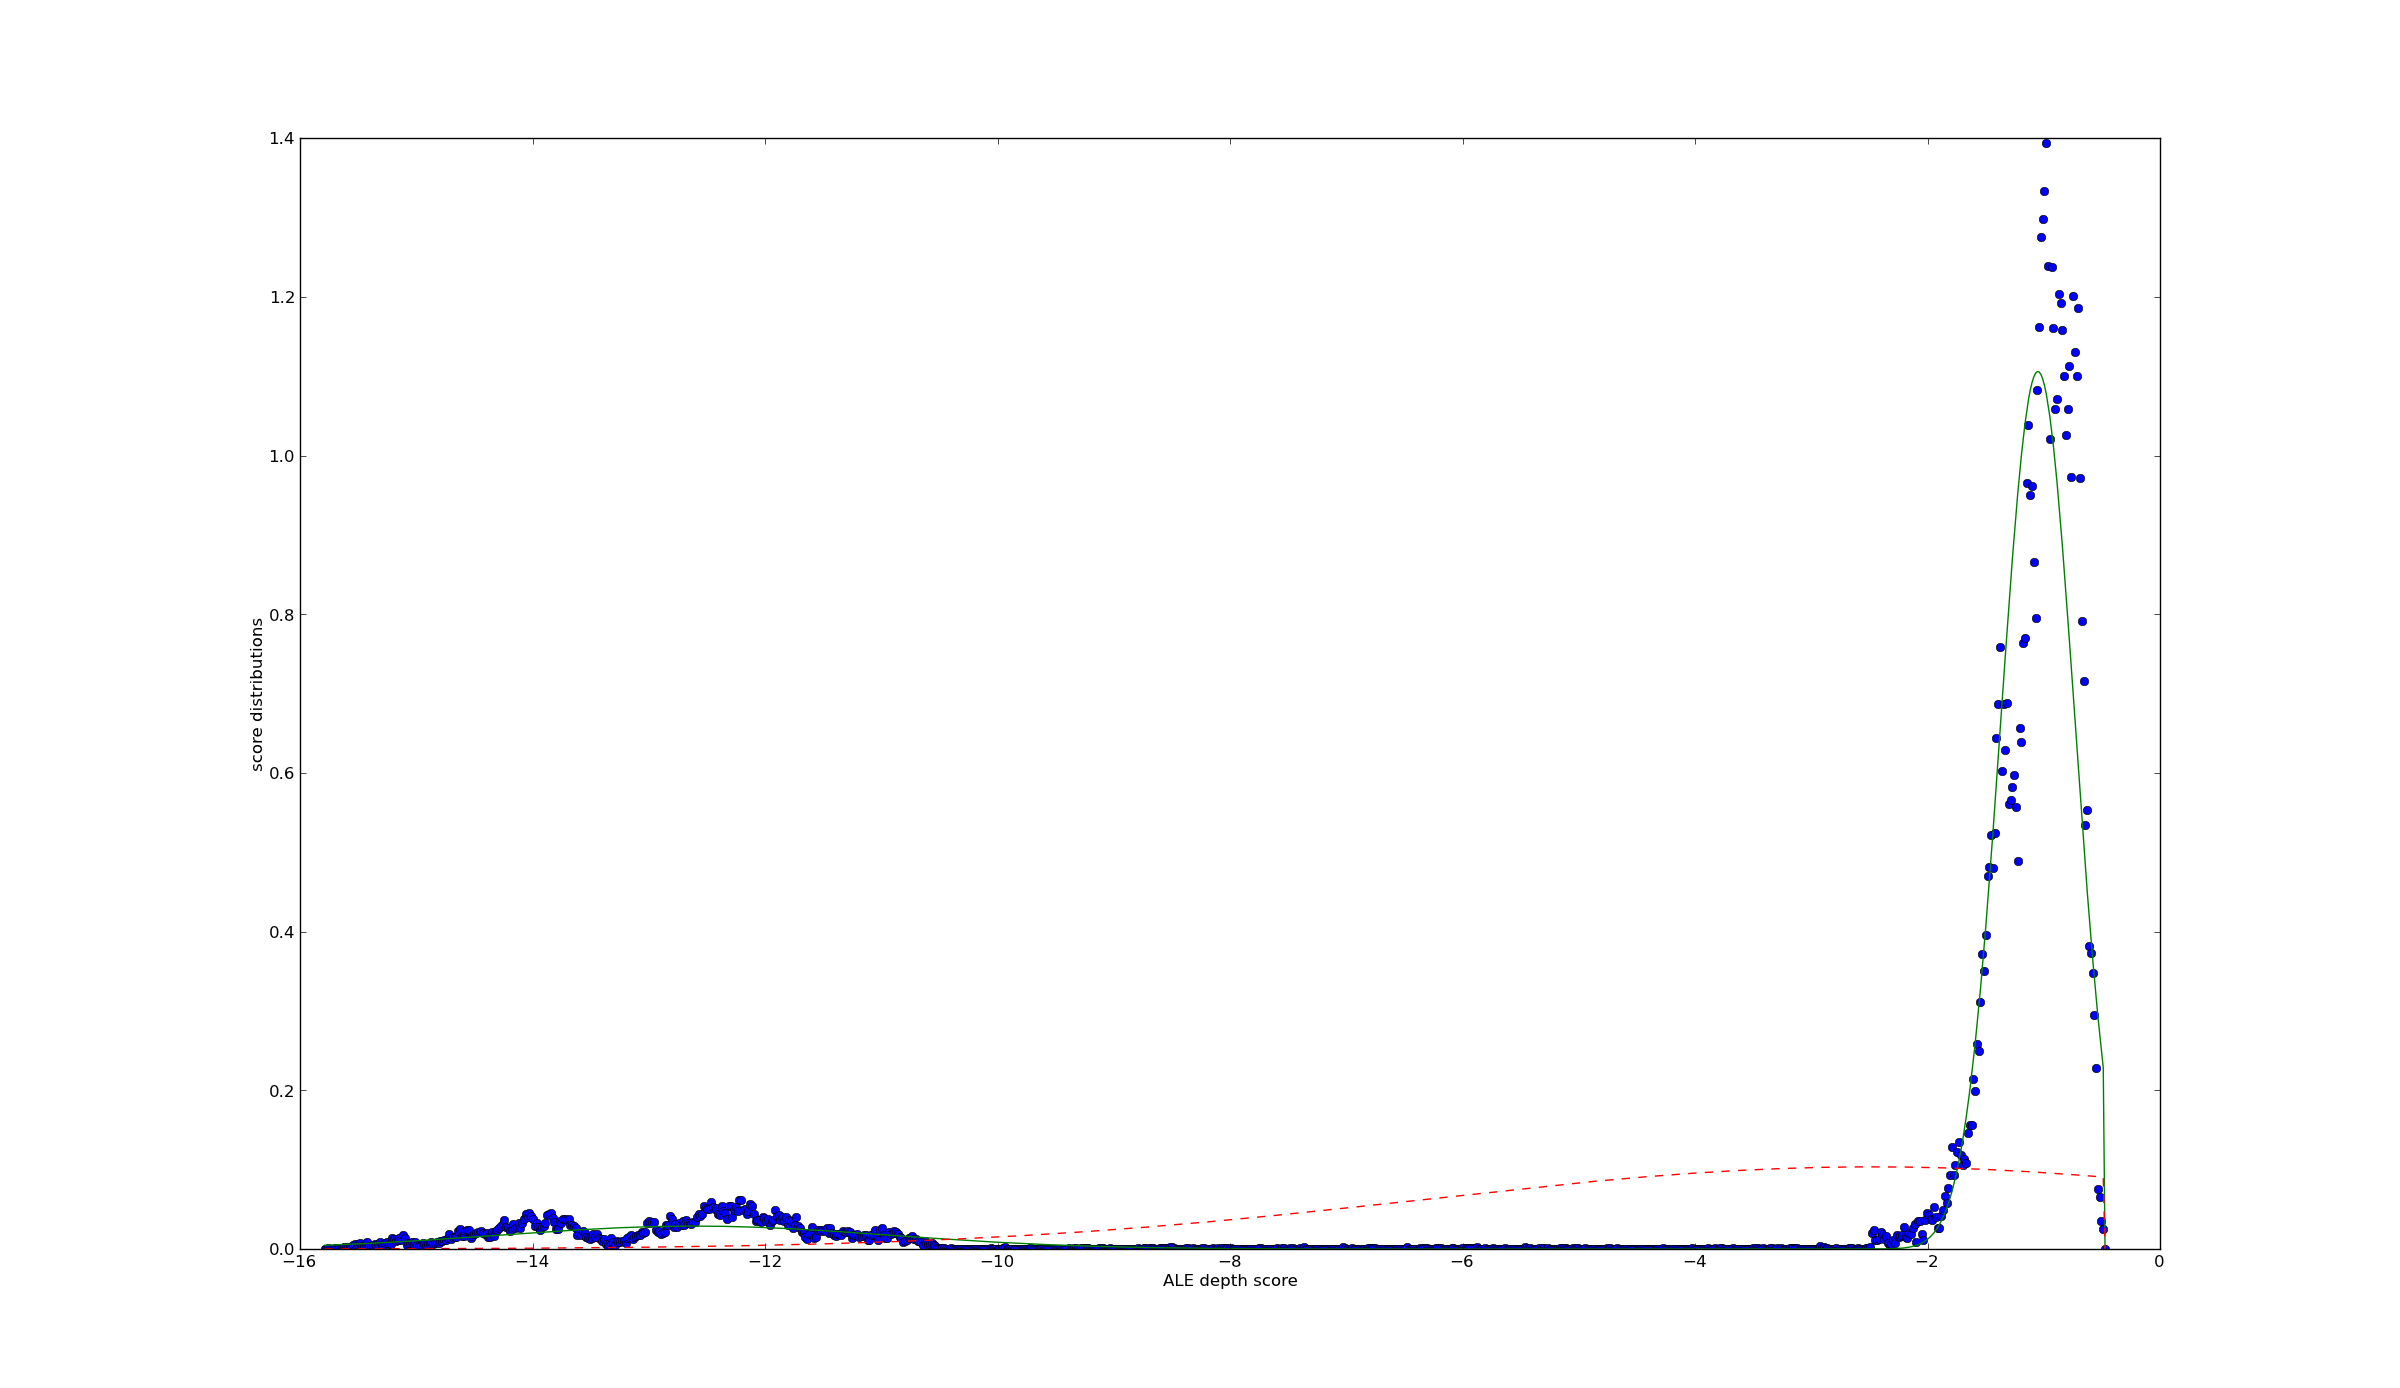
\includegraphics[width=\textwidth]{figures/ALE/gmm_spiro_depth.png}}
    \caption[Example of GMM for ALE depth score]{We see the difference between the observed depth scores (blue dots), the two component Gaussian mixture model (green line) and a single component Gaussian mixture model (red dashed line). It is clear that the mixture model is a far superior fit to the data}
 	\label{fig:GMM_spiro}
\end{figure}

\begin{table}[hpt]

    \begin{center}
    \begin{tabular}{c|c|c}
        & 2-Gaussian mixture & single Gaussian \\
        \hline
        $\mu$ & -12.56, -1.05 & -2.47 \\
        $\sigma^{2}$ & 1.72, 0.32& 3.85 \\
        $\log(p)$ & -42627.63 & -12771185.48
    \end{tabular}
\end{center}
\caption[Example of GMM for ALE depth score]{The components and log likelihoods of the two models. We can see that the two Gaussian mixture model is 2 orders of magnitude more likely (in log space) than the single Gaussian model.}
\label{tab:GMM_spiro}
\end{table}

\section{False positive rate vs. number of reported errors}
\label{ROCALE}

In section \ref{SNVsReal} the values given were for the top 0.0001\% and top 0.0005\% of lowest ALE scoring positions. These values were arbitrarily chosen (and can be set by the user in the software package). In Figure \ref{fig:ROC_ALE} we see how the number of reported lowest scoring positions affects the sensitivity and accuracy of ALE with respect to the manually curated set of errors.

Of the top 250 positions on chromosome 1 with the lowest ALE placement score, 88\% of
them are within an insert length (200bp) of either a hard stop (0 depth) or a variant. Furthermore,
these 250 positions are within an insert length of 84\% of the variants and we find 58\% at the
exact base ALE reports. This is to say that we are able to independently locate 154 of 176
variants with a false positive rate of 12\% within the first 250 lowest ALE placement scores. For
chromosome 2 the lowest 75 ALE placement score positions return 85\% (41 of 46) of the variants
(60\% exactly) with an 11\% false positive rate. As a whole ALE discovers 188 of the 222 variants
with a false positive rate of 12\%.

In figure \ref{fig:ROC_ALE} we can see how the total number of lowest ALE placement scores observed
changes the number of variants that we correctly reproduce and the total true positive rate. As
we look at more positions we recover more variants, but with a higher rate of false positives.
Depending on the number of errors in the genome, the slope at which the true positive rate
decreases will vary. A binary search for an acceptable false positive rate can be performed to
meet the needs of accuracy in individual projects.

\begin{figure}[hpt]
 	\centerline{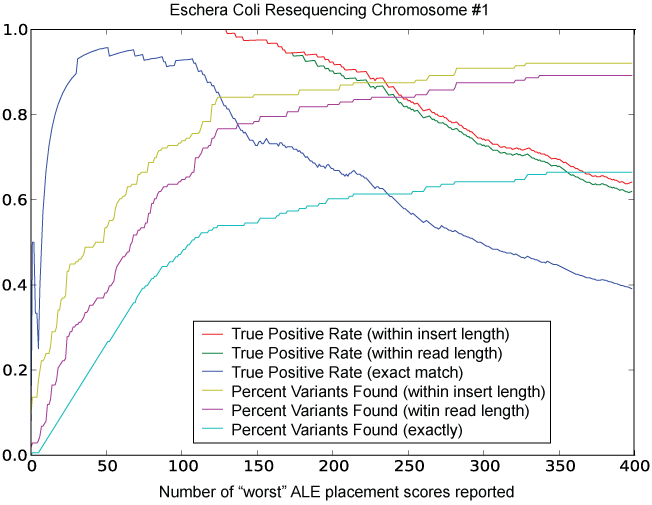
\includegraphics[width=\textwidth]{figures/ALE/fig6_top.png}}
    \caption[ROC curve vs. number of reported errors]{We use ALE to score a re-sequencing genome of {\it E.Coli} in which a set of errors has
been manually and independently curated. The top X lowest ALE placement scores at positions
where there is at least a single read correspond well to the variants discovered in genome
finishing. As we increase the number of ALE scores examined the total percent of variants found
exactly and within a read (36bp) or insert (200bp) length increases. The top area corresponding to
these low scores tend to contain, or is within a short distance of a variant or a “hard stop” (region
of 0 depth). This is to say that the true positive rate is very high (false positive rate very low). This figure
shows how the various rates change with the number of ALE scores reported for Chromosome 1
of the {\it E.Coli} re-sequencing project. We see that after 150 positions that most variants are found,
but we still have a very low false positive rate.}
 	\label{fig:ROC_ALE}
\end{figure}

\begin{figure}[hpt]
    \centerline{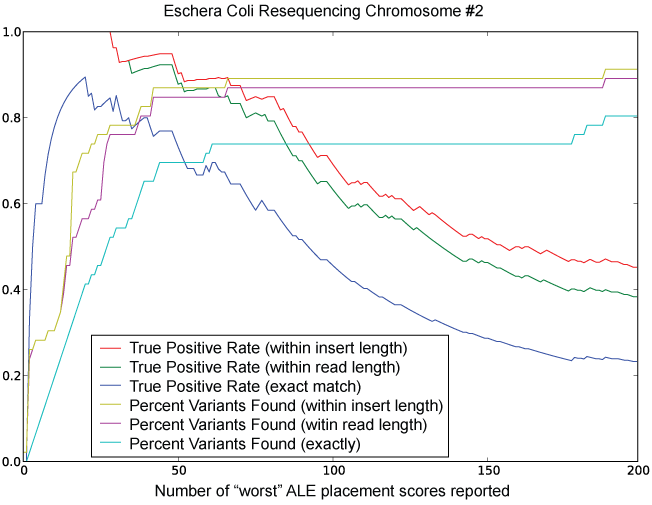
\includegraphics[width=\textwidth]{figures/ALE/fig6_bot.png}}
    \caption[ROC curve for chromosome 2]{Similar to Figure \ref{fig:ROC_ALE}, for Chromosome 2, which is smaller,
after only 75 scores most variants are discovered and the false positive rate is around 10\%. As we
look at more scores we discover more variants, but the false positive rate increases.}
 	\label{fig:ROC_ALE2}
\end{figure}

\section{Influence of alignment input} % (fold)
\label{sec:Influence of alignment input}

ALE takes as input a proposed assembly and a SAM/BAM \cite{Li2009} file of alignments of reads onto this proposed assembly. This allows ALE to calculate the probability of observing the assembly given the reads. ALE assumes that this mapping will include, if not all possible mappings, at least the ``best" mapping for each read in the library (if such a mapping exists). For assemblies with many repeat regions (>100) or libraries with large insert sizes, this can be difficult to obtain due to the bias introduced using default parameters of standard aligners. While an extensive review of alignment packages and their optimization is beyond the scope of this work, a review can be found in \cite{Li2010}. If an assembly has many repeats and the aligner bias causes the reporting of reads only mapping to a fraction of possible regions, then ALE will see the unmapped regions as having 0 depth (no supporting reads) which will result in artificially low depth sub-scores. The robustness of ALE will still allow for comparison between assemblies with similar biases, but should be taken into account if the input to ALE is biased for only certain assemblies. To avoid this bias some mappers must be explicitly forced to search for all possible placements (-a in bowtie).

In summary, ALE determines the likelihood of an assembly given the reads and an accurate, unbiased alignment of those reads onto the assembly, without which the model assumptions are violated. These preconditions are usually met except for certain pathological genomes, and even in these cases can be readily corrected by changing the parameters of the aligner used to make ALE's input.

% section Influence of alignment input (end)

\section{Depth Z normalization} % (fold)
\label{sec:DepthZnormalization}

When calculating $\hat{Z}_{\text{depth}}$ at a specific position analytically,
\begin{equation}
    \hat{Z}_{\text{depth}}(r,k) = \sum_{k=0}^{\infty} \left(\mbox{nbPMF}\left(k,r,\frac{1}{2}\right)\right)^{2} = \frac{1}{4^{r}} \ _{2}\mbox{F}_{1}\left(r,r;1;\frac{1}{4}\right)
\end{equation}
where $r$ is the depth, $k$ is the expected depth, $_{2}\mbox{F}_{1}$ is a hyper geometric function,
\begin{equation}
    _{2}\mbox{F}_{1}\left(r,r;1;\frac{1}{4}\right) = \sum_{n=0}^{\infty} \frac{(r)^{2}_{n}}{4^{n}n!(1)_{n}}
\end{equation}
where
\begin{equation}
    (r)_{n} = \frac{\Gamma(r+n)}{\Gamma(r)}    
\end{equation}
and nbPMF is the negative binomial probability mass function
\begin{equation}
    \mbox{nbPMF}\left(k,r,p\right) = {k+r-1 \choose k} (1-p)^{r}p^{k}.
\end{equation}

We note that numerically evaluating this function results in precision errors for large $r$ due to the fact that we are multiplying a very small number by a very large number. If we move the fraction into the hyper-geometric function and take the exponential of the log we get
\begin{equation}
    \hat{Z}_{\text{depth}}(r) = \sum_{n=0}^{\infty} \exp\left(2S(r+n) - 2S(r) - 2S(n+1) - (r+n)\log(4)\right)
\end{equation}
where
\begin{equation}
    S(x) = \log\left(\Gamma(x)\right)
\end{equation}
and we can use Stirling's approximation,
% return (input - 0.5)*log(input) - input + lnfactconst2 + 1.0/(12.0*input) - 1.0/(360.0*input3) + 1.0/(1260.0*input5) - 1.0/(1680.0*input7);
\begin{equation}
    S(x) = \log\left(x - \frac{1}{2}\right)\log(x) - x + \log(2\pi) + \frac{1}{12x} - \frac{1}{360x^{3}} + \frac{1}{1260x^{5}} - \frac{1}{1680x^{7}} + O\left(\frac{1}{x^{9}}\right)
\end{equation}
to estimate this value. The sum is calculated in practice from $n=0$ until the resulting contribution is less than machine precision ($10^{-16}$ for doubles) due to the fact that the interior function is monotonically decreasing. This is pre-computed in python for common values of $r$ (0 to 2048) for constant time lookup. Other values are computed in real time as needed.

This allows us to numerically calculate $\hat{Z}_{\text{depth}}$ with high precision.

% section Depth Z normalization (end)

\section{Availability and requirements}
 \begin{itemize}
  \item \textbf{Project name:} ALE
  \item \textbf{Project home page:} www.alescore.org (and www.github.com/sc932/ALE)
  \item \textbf{Operating systems:} Linux 32/64-bit, Mac OSX, Windows (Cygwin)
  \item \textbf{Programming languages:} Python, C
  \item \textbf{Other requirements:} Some python packages, see documentation
  \item \textbf{License:} UoI/CNSA Open Source
 \end{itemize}

% chapter ALE Implementation (end)

% part ALE: Assembly Likelihood Evaluation (end)

\part{EPI: Expected Parallel Improvement} % (fold)
\label{prt:EPI: Expected Parallel Improvement}
\singlespacing

\noindent
\Large
EPI: Expected Parallel Improvement

\noindent
\normalsize
Joint work with Peter Frazier$^{1}$ \\
\scriptsize
$^{1}$Cornell University School of Operations Research and Information Engineering, Ithaca, New York 14853, USA
\normalsize

\normalspacing

\begin{center}
   Abstract 
\end{center}

This derivative-free global optimization method allows us to optimally sample many points concurrently from an expensive to evaluate, unknown and possibly non-convex function. Instead of sampling sequentially, which can be inefficient when the available resources allow for simultaneous evaluation, EPI provides the best set of points to sample next, allowing multiple samplings to be performed in unison.

In this work we develop a model for expected parallel improvement based on numerically estimating the expected improvement using multiple samples and use multi-start gradient descent to find the optimal set of points to sample next, while fully taking into account points that are currently being sampled for which the result is not yet known.

\chapter{EPI Introduction} % (fold)
\label{cha:EPI Introduction}

\section{Optimization of Expensive Functions}

Optimization attempts to find the maximum or minimum value of some function or experiment. The goal is to find the input or set of parameters that either maximizes or minimizes a particular value. This can be maximizing gains in a financial model, minimizing costs in operations, finding the best result of a drug trial or any of a number of real world examples. The basic setup is that there is something that is desirable to maximize or minimize and we want to find the parameters that obtain this. The underlying functions may be difficult to sample; whether requiring long amounts of time such as drug trials, or excessive money such as financial models, or both such as exploration of natural resources. This limitation forces a good optimization algorithm to find the best possible solution quickly and efficiently, requiring as few exploratory samplings as possible before converging to an optimal solution.

The quantitative and data-intensive explosion in fields such as bioinformatics and other sciences is producing petabytes of data and increasingly complex models and computer algorithms to analyze it. As the amount of data being inputed and the complexity of these algorithms grow they take more and more time to compute. Even with modern supercomputers that can perform many peta-FLOPS ($10^{15}$ Floating Point Operations Per Second) scientific codes simulating fluid dynamics \cite{Compo2011} and complex chemical reactions \cite{Valiev2010} can take many hours or days to compute, using millions of CPU hours or more. The assembly of a single genome using the software package Velvet \cite{Zerbino2008} can take 24 hours or more on a high memory supercomputer. The sheer amount of time and resources required to run these simulations and computations means that the fine-tuning of the parameters of the models is extremely time and resource intensive.

Statistical methods such as EGO \cite{Jones1998} attempt to solve this problem by estimating the underlying function that is being optimized and computing the next point to sample so that it maximizes the expected improvement over the best result observed so far. When performed sequentially, this method often quickly finds a good point within the space of possible inputs, and given more samples will continue to search for the global optimum. This method is limited by its sequential nature, however, and cannot take advantage of possible parallel computational or sampling resources allowing for samples to be drawn concurrently. There have been some heuristic attempts to address the problem of parallel expected improvement \cite{Ginsbourger2008}, but all suffer from limitations in their sequential design. In this work we develop a model for expected parallel improvement, based on numerically estimating expected improvement using multiple samples and use multi-start gradient descent to find the optimal set of points to sample next, while fully taking into account points that are currently being sampled for which the result is not yet known.

\section{Gaussian Processes}

We begin with a Gaussian process prior on a continuous function $f$. The function $f$ has domain $A \subseteq \mathbb{R}^{d}$. Our overarching goal is to solve the global optimization problem

\begin{equation}
\max_{x \in A} f(x).
\end{equation}
This problem can be constrained or unconstrained depending on the set $A$.

The paper \cite{Jones1998} developed a method for choosing which points to evaluate next based on fitting a global metamodel to the points evaluated thus far, and then maximizing a merit criterion over the whole surface to choose the single point to evaluate next.

Although \cite{Jones1998} describes their technique, EGO, in terms of a kriging metamodel and uses frequentist language, their technique can also be understood in a Bayesian framework. This framework uses a Gaussian process prior on the function $f$, which is a probabilistic model whose estimates of $f$ have the corresponding framework described below.

\section{Gaussian process priors}

Any Gaussian process prior on $f$ is described by a mean function $\mu : A \mapsto \mathbb{R}$ and a covariance function $K : A \times A \mapsto \mathbb{R}_{+}$. The mean function is general, and sometimes reflects some overall trends believed to be in the data, but is more commonly chosen to be 0. The covariance function must satisfy certain conditions: 

\begin{equation}K(x,x) \geq 0,\end{equation}
\begin{equation}K(x,y) = K(y,x),\end{equation}

    and it must be positive semi-definite, which is to say that for all $\vec{x}_{1}, \ldots, \vec{x}_{k} \in A$, and all finite $k$, if we construct a matrix by setting the value at row $i$ and column $j$ to be $\Sigma_{ij} = K(\vec{x}_{i}, \vec{x}_{j})$ this matrix must be positive semi-definite,

\begin{equation}\vec{v}^{T}\Sigma \vec{v} \geq 0, \ \ \ \forall \vec{v} \in \mathbb{R}^{d}.\end{equation}

Common choices for $K$ include the Gaussian covariance function, $K(x,x^{\prime}) = a \exp(-b \| x - x^{\prime}\|^{2})$ for some parameters $a$ and $b$ and the power exponential error function, $K(x, x^{\prime}) = a \exp(-\sum_{i} b_{i} (x_{i} - x_{i}^{\prime})^{p})$ for some parameters $\vec{b} \in \mathbb{R}^{d}, p$ and $a$.

Putting a Gaussian Process (GP) prior on $f$, written
\begin{equation}
 f \sim \mbox{GP}(\mu(\cdot), K(\cdot, \cdot))
\end{equation}
means that if we take any fixed set of points $x_{1}, \ldots, x_{n} \in A$ and consider the vector $(f(x_{1}), \ldots, f(x_{n}))$ as an unknown quantity, our prior on it is the multivariate normal,
\begin{equation}
    (f(x_{1}), \ldots, f(x_{n})) \sim N\left( \left[ \begin{tabular}{c} $\mu(x_{1})$ \\ $\vdots$ \\ $\mu(x_{n})$ \end{tabular} \right] , \Sigma_{n} = \left[ \begin{tabular}{ccc} $K(x_{1}, x_{1})$ & $\cdots$ & $K(x_{n}, x_{1})$ \\ $\vdots$ & $\ddots$ & $\vdots$ \\ $K(x_{1}, x_{n})$ & $\cdots$ & $K(x_{n},x_{n})$ \end{tabular} \right] \right).
\end{equation}

GPs are analytically convenient. If we observe the function $f$ at $x_{1}, \ldots, x_{n}$, getting values $y_{1} = f(x_{1}), \ldots, y_{n} = f(x_{n})$, then the posterior of $f$ is also a GP,
\begin{equation}
 f|x_{1:n}, y_{1:n} \sim GP(\mu_{n}, \Sigma_{n})
\end{equation}
where $\mu_{n}$ and $\Sigma_{n}$ are defined in the Methods section \ref{comp_of_gp}. We can see the evolution of the GP as more points are sampled in Figure \ref{fig:GPP_evolve}.

\begin{figure}[hpt]
 	\centerline{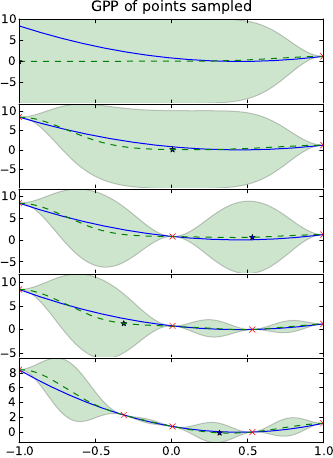
\includegraphics[width=0.75\textwidth]{figures/EPI/GPP_stepper_EI.png}}
    \caption[Evolution of a GPP]{We can watch the GPP mean (green dashed) and variance (green shaded) evolve to become closer and closer to the true function (blue line) as more and more samples (red x) are drawn from the function. The mean adapts to fit the points sampled and the variance is lowest near sampled points.}
 	\label{fig:GPP_evolve}
\end{figure}

\section{Expected Improvement}

When considering where to measure next, the EGO algorithm, and more generally the Expectation Improvement (EI) criterion, computes a merit function defined as
\begin{equation}
 \mbox{EI}(x) = \mathbb{E}_{n} \left[\left[ f_{n}^{\star} - f(x) \right]^{+} \right] = \mathbb{E} \left[ f_{n}^{\star} - f_{n+1}^{\star}| x_{n} = x\right]
\end{equation}
where $f_{n}^{\star} = \min_{m \leq n} f(x_{m})$.

This is the point where we expect the greatest improvement to the best point sampled so far, $f_{n}^{\star}$. The algoritm attempts to maximize the EI at every iteration, sampling only the points with the greatest potential return. In Figure \ref{fig:GPP_EI_evolve} we show the values of EI for the GPP in Figure \ref{fig:GPP_evolve}.

\begin{figure}[hpt]
 	\centerline{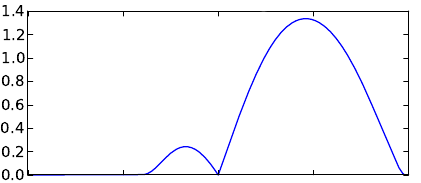
\includegraphics[width=0.75\textwidth]{figures/EPI/GPP_example_EI4.png}}
    \centerline{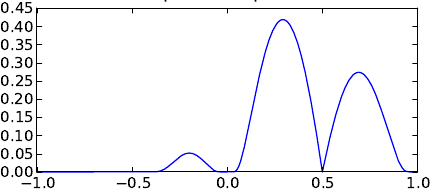
\includegraphics[width=0.75\textwidth]{figures/EPI/GPP_example_EI.png}}
    \caption[Evolution of expected improvement of a GPP]{The expected improvement of panels 4 and 5 of Figure \ref{fig:GPP_evolve}. We can see that regions with low mean and high variance have the highest expected improvement.}
 	\label{fig:GPP_EI_evolve}
\end{figure}

\subsection{Parrallel Heuristics}

The inherent downside to the EGO algorithm is that it is sequential; it results in only a single proposed sample point, which must be sampled before a new point can be proposed. This is a waste of resources if many points can be sampled simultaneously. Under the EGO algorithm these excess resources would sit idle while each point is sampled one at a time.

There are a few heuristic extensions to the EGO algorithm that attempt to alleviate this bottleneck including the {\it constant liar} and {\it kriging believer} methods proposed by \cite{Ginsbourger2008}.

\subsubsection{Constant liar heuristic}

In this heuristic the points that are currently being sampled are all artificially set to a constant value like $\min(\vec{y}), \max(\vec{y})$ or mean$(\vec{y})$ and then normal EI maximization is performed. This method fails to accurately account for the subtleties of the model and information that the GPP provides at each location.

\subsubsection{Kriging believer heuristic}

In this heuristic the points being sampled are assumed to return a value equal to their expectation, effectively lowering the variance to 0 at the given point. This method fails to account for the variability at the points sampled, and the way this variability affects the value of additional evaluations at other points.

\section{Expected Parallel Improvement}

We propose to extend the EI algorithm to be used in parallel systems, where we can evaluate several function values simultaneously on different cores, CPUs or GPGPUs. Instead of having to pick a single point to sample next, we can pick several.

The core of this idea is that we can calculate the expected improvement for simultaneous evaluation of points $x_{n+1}, \ldots, x_{n+l} = \vec{x}$ as
\begin{equation}
 \mbox{EI}(x_{n+1}, \ldots, x_{n+l}) = \mathbb{E}_{n}\left[\left[f_{n}^{\star} - \min\left\{f(x_{n+1}), \ldots, f(x_{n+l})\right\}\right]^{+}\right].
\end{equation}
The optimization then approximates the solution to
\begin{equation}
 \argmin_{\vec{x} \in \mathbb{R}^{d \times l}} \mbox{EI}(\vec{x}),
\end{equation}
and chooses this batch of points to evaluate next. While the purely sequential case allows straightforward analytic evaluation of $\mbox{EI}(x)$, calculating $\mbox{EI}(\vec{x})$ in the parallel case is more challenging and requires numerical estimation. Although straightforward estimation via standard Monte Carlo are inefficient, we deploy several techniques to more accurately estimate and optimize $\mbox{EI}(\vec{x})$.

% chapter EPI Introduction (end)

\chapter{EPI Methods} % (fold)
\label{cha:EPI Methods}

\section{Components of the Gaussian Prior}
\label{comp_of_gp}

In the following sections we will explicitly define the mean (Section \ref{methods_GP_mean}) and variance (Section \ref{methods_GP_var}) of the GP, as well as their component-wise gradients. We will also define the partial derivatives for our default covariance function, the squared exponential covariance in Section \ref{methods_GP_cov}.

\subsection{The GP mean}
\label{methods_GP_mean}

First we try to decompose the GP mean in order to easily find an analytic expression for its gradient:
\begin{equation}
 \vec{\mu_{\star}} = K(\vec{x}_{\star}, \textbf{X} )K(\textbf{X},\textbf{X})^{-1}\vec{y}.
\end{equation}
Where $\textbf{X}$ is the matrix whose rows are composed of a collection of vectors in $A$. We define the matrix $K(\vec{y}, \vec{z})$ component-wise as
\begin{equation}
    K(\vec{y}, \vec{z})_{ij} = K(\vec{y}_{i}, \vec{z}_{j}).
\end{equation}
We note that if $\vec{x_{\star}}$ is a single point then the matrix $K(\vec{x}_{\star}, \textbf{X} )$ collapses to a vector. We also rewrite $K(\textbf{X},\textbf{X})^{-1}$ as $K^{-1}$ for simplicity,
\begin{equation}
 \vec{\mu_{\star}} = K(\vec{x}_{\star}, \textbf{X} ) K^{-1} \vec{y}.
\end{equation}
We further note that we can decompose the resulting vector dot product into a sum for each component of $\vec{\mu_{\star}}$,
\begin{equation}
 \mu_{\star {i}} = \sum_{j = 1}^{N} K(x_{\star i}, X_{j}) \left(K^{-1} \vec{y} \right)_{j}.
\end{equation}

When we take the gradient, we note that it can be brought inside the sum and the vector $(K^{-1}\vec{y})$ is constant with respect to $x_{\star}$,
\begin{equation}
 \frac{\partial}{\partial x_{\star t}} \mu_{\star i} = \sum_{j = 1}^{N} \left(K^{-1} \vec{y} \right)_{j} \frac{\partial}{\partial x_{\star t}} K(x_{\star i}, X_{j}).
\end{equation}
We note that
\begin{equation}
\frac{\partial}{\partial x_{\star t}} \mu_{\star i} = \left\{ \begin{tabular}{cc}
                                                                  $\sum_{j = 1}^{N} \left(K^{-1} \vec{y} \right)_{j} \frac{\partial}{\partial x_{\star i}} K(x_{\star i}, X_{j})$ & for $i = t$ \\
								  0 & otherwise
                                                                 \end{tabular}\right..
\end{equation}

\subsection{The GP variance}
\label{methods_GP_var}

Now we do the same thing for the covariance which is defined as
\begin{equation}
 K(\mu_{star}) = K(\textbf{X$_{\star}$}, \textbf{X$_{\star}$}) - K(\textbf{X$_{\star}$}, \textbf{X}) K(\textbf{X}, \textbf{X})^{-1} K(\textbf{X}, \textbf{X$_{\star}$}).
\end{equation}
The components $(i,j)$ of $\Sigma$ (see Section \ref{EPI_imp_var}) are
\begin{equation}
 \Sigma_{ij} = K(x_{\star i}, x_{\star j}) - \sum_{p = 1}^{N} \sum_{q = 1}^{N} K^{-1}_{qp} K(x_{\star i}, X_{q}) K(x_{\star j}, X_{p})
\end{equation}
and the derivative $\frac{\partial}{\partial x_{\star t}} \Sigma_{ij}$ becomes
\begin{equation}
 \frac{\partial}{\partial x_{\star t}} K(x_{\star i}, x_{\star j}) - \\
 \sum_{p = 1}^{N} \sum_{q = 1}^{N} K^{-1}_{qp} \left( K(x_{\star i}, X_{q}) \frac{\partial}{\partial x_{\star t}} K(x_{\star j}, X_{p}) + K(x_{\star j}, X_{p}) \frac{\partial}{\partial x_{\star t}} K(x_{\star i}, X_{q}) \right)
\end{equation}
For a more detailed discussion see Section \ref{EPI_imp_var}.

\subsection{Defining the covariance derivatives}
\label{methods_GP_cov}

A common function for the covariance is the squared exponential covariance function,
\begin{equation}
    K(x_{i}, x_{j}) = \sigma_{f}^{2}\exp\left( -\frac{1}{2l^{2}} |x_{i} - x_{j}|^{2}\right)  + \sigma_{n}^{2}\delta_{ij},
\end{equation}
where $\delta_{ij}$ is the Kronecker delta,
\begin{equation}
    \delta_{ij} = \left\{ \begin{tabular}{ccc}
        1 & if & $i=j$ \\
        0 & if & $i\neq j$
    \end{tabular} \right..
\end{equation}
We will use an instance of this covariance function where $l$ is a length scale, $\sigma_{f}^{2}$ is the signal variance, and $\sigma_{n}^{2}$ is the sample variance. The maximum likelihood of these parameters can be determined from the training data as seen in section \ref{sec:Adaptation of hyperparameters}. We will treat them as constants for now.

It will be sufficient to show the partial derivative of one of the variables because cov$(x_{i}, x_{j}) = $ cov$(x_{j}, x_{i})$.
\begin{equation}
    \frac{\partial}{\partial x_{i}} K(x_{i}, x_{j}) = \delta_{ij} + \frac{\partial}{\partial x_{i}} \sigma_{f}^{2} \exp\left( - \frac{1}{2l^{2}} |x_{i} - x_{j}|^{2}\right)
\end{equation}
\begin{equation}
    =  \delta_{ij} + \frac{-\sigma_{f}^{2}}{2l^{2}} \exp\left( - \frac{1}{2l^{2}} |x_{i} - x_{j}|^{2}\right) \frac{\partial}{\partial x_{i}} |x_{i} - x_{j}|^{2}
\end{equation}
\begin{equation}
    =  \frac{x_{j} - x_{i}}{l^{2}} K(x_{i}, x_{j}) + \delta_{ij}.
\end{equation}

\section{Estimation of expected improvement}
\label{estEI}

We estimate the expected improvement at a set of points $\vec{x}$ by sampling from the GP over many Monte Carlo iterations.

The mean $\vec{\mu}$ and covariance $\Sigma$ of the points to be sampled $\Sigma$ is defined in section \ref{methods_GP_mean} and \ref{methods_GP_var}.

We can simulate drawing points from this multivariate gaussian like so,
\begin{equation}
    \vec{y}^{\prime} = \vec{\mu} + L \vec{w}
\end{equation}
where $L$ is the Cholesky decomposition of $\Sigma$ and $\vec{w}$ is a vector of independent, identically distributed normal variables with mean 0 and variance 1.

The improvement from this simulated sample is
\begin{equation}
    I^{\prime} = \left[f_{n}^{\star} - \min(\vec{y}^{\prime})\right]^{+}.
\end{equation}
By averaging over many such simulated draws we can accurately estimate the expected improvement for the set of points $\vec{x}$. Further discussion and analysis of the accuracy of this method is discussed in section \ref{GPUEI}.


\section{Estimation and optimization of $\mbox{EI}(\vec{x})$}

To optimize $\mbox{EI}(\vec{x})$, we calculate stochastic gradients
\begin{equation}
 g(\vec{x}) = \bigtriangledown \mbox{EI}(\vec{x})
\end{equation}
and use infinitesimal perturbation analysis \cite{Fu1994} to interchange derivative and expectation, see section \ref{EPI_proof}. Then use multistart gradient descent to find the set of points that maximize $\mbox{EI}(\vec{x})$, see section \ref{sec:multistart}.

\subsection{Interchange of gradient}
\label{EPI_proof}

Let $\vec{x} = \left(\vec{x}_{1}, \ldots, \vec{x}_{l}\right)$ and
\begin{equation}
    Z \left(\vec{x}\right) = \left[f_{n}^{\star} - \min_{i = 1,\ldots,l} f \left(\vec{x}_{i}\right)\right]^{+}
\end{equation}
with
\begin{equation}
    f_{n}^{\star} = \min_{m\leq n} f \left(\vec{x}_{m}\right).
\end{equation}
Then
\begin{equation}
    EI_{n}(\vec{x}) = \mathbb{E}_{n}\left[Z \left(\vec{x}\right)\right].
\end{equation}

We conjecture
\begin{equation}
    \nabla \left[\mathbb{E}_{n}\left[Z \left(\vec{x}\right)\right]\right] = \mathbb{E}_{n}\left[\nabla Z \left(\vec{x}\right)\right] =  \mathbb{E}_{n}\left[g_{n}(\vec{x})\right]
\end{equation}
for all $\vec{x}$ with $\vec{x}_{i} \neq \vec{x}_{j}$ for every $i \neq j$.

We have
\begin{equation}
    g_{n}(\vec{x}) = \left\{ \begin{tabular}{ccc}
        0 & if & $i^{\star}(\vec{x}) = 0$ \\
        $-\nabla_{\vec{x}} f(\vec{x}_{i})$ & if & $i^{\star}(\vec{x}) = i$
    \end{tabular} \right.
\end{equation}
and
\begin{equation}
    i^{\star}(\vec{x}) = \left\{ \begin{tabular}{ccc}
        0 & if & $f_{n}^{\star} \leq \min_{i=1,\ldots,l} f(\vec{x}_{i})$ \\
        $\min \argmin_{i=1,\ldots,l} f(\vec{x}_{i})$ & & otherwise.
    \end{tabular} \right.
\end{equation}
and leave the proof for a later publication.

\section{Multistart gradient descent}
\label{sec:multistart}

We use multistart gradient descent to find the set of points that maximizes the parallel expected improvement over some number of total restarts $R$.

For each multistart iteration we draw the initial points $\vec{x}^{(t=0)}$ from a Latin hypercube. The update formula for each $\vec{x}_{i}$ in the set of proposed points to sample is
\begin{equation}
    \vec{x}_{i}^{(t+1)} = \vec{x}_{i}^{(t)} + \frac{a}{t^{\gamma}} \nabla_{\vec{x}_{i}} {\rm EI}\left(\vec{P}^{(t)} | \vec{X}\right)
\end{equation}
where $a$ and $\gamma$ are parameters of the gradient descent model. $\vec{P}^{(t)}$ is the union of the set of points being currently sampled and the proposed new points to sample. This update is performed for some set number of iterations, or until
\begin{equation}
    \left|\vec{x}_{i}^{(t+1)} - \vec{x}_{i}^{(t)}\right| < \epsilon
\end{equation}
for some threshold $\epsilon > 0$.

After $R$ restarts, the set of points with the best expected EI is chosen as the set of points to sample next. Figure \ref{fig:pk_paths} shows the paths of 128 multistart gradient descent paths with $l = 2$ on the EI of the Branin function.

\begin{figure}[hpt]
 	\centerline{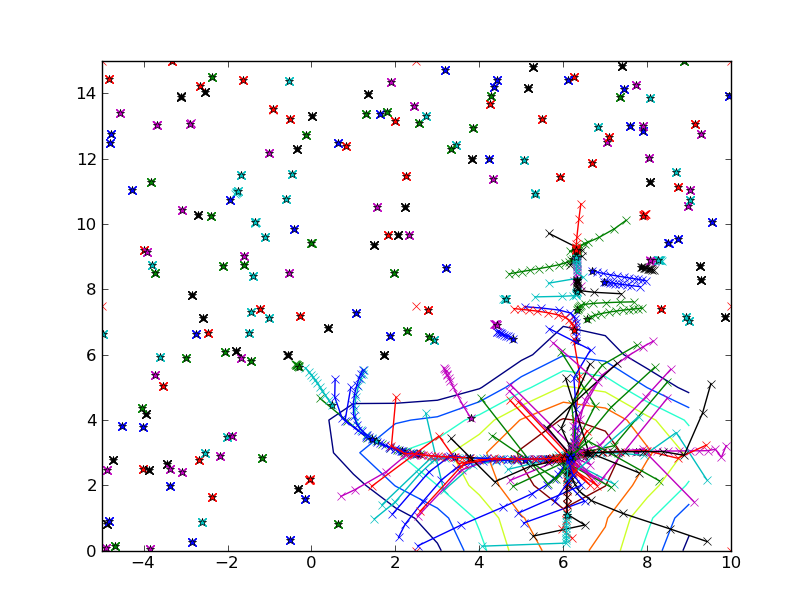
\includegraphics[width=\textwidth]{figures/EPI/branin_2d_32pk_paths_and_EI.png}}
    \caption[Gradient descent paths in Branin Function]{The gradient descent paths of 2 points (simulating 2 free cores, $l=2$) with initial points chosen from a Latin hypercube of the domain over 128 restarts (each color represents a different restart). The EI of the function is shown as a contour plot. We see the paths converging on the point of highest EI.}
 	\label{fig:pk_paths}
 \end{figure}

 We note that some points appear to not move in Figure \ref{fig:pk_paths}. This happens when one of the points has a very high expected evaluation value under the GP. This causes that point to not contribute to the EI, and therefore the gradient of the EI with respect to that point is low, or zero, causing it to remain stationary while the other point rushes to the maximum EI (from section \ref{estEI}).


% chapter EPI Methods (end)

\chapter{EPI Results} % (fold)
\label{cha:EPI Results}

In this chapter we will present preliminary results using the EPI algorithm and software package. The research is ongoing and the full results will be published in a forthcoming paper with Peter Frazier.

%TODO graphs showing gain vs wallclock time

\section{Parallel speedup using function drawn from prior}

To test the speedup obtained by using EPI over serial methods such as EGO we generate a set of test functions from a 1-D prior and determine the average improvement at each wall clock unit of time for EGO and EPI running with 2, 4 and 8 cores. Each wall clock unit of time represents $n$ samplings of the function where $n$ is the number of cores being used.

We can see in Figure \ref{fig:EPI_res1} that the number of cores (or concurrent experiments) is directly proportional to the ending average improvement after a set number of wall clock time ($t = 10$). Future work includes refining these results, increasing the maximum number of cores and testing EPI against other heuristics in this and higher dimensional spaces.

%TODO
%more cores, more samples, more MC runs
\begin{figure}[hpt]
 	\centerline{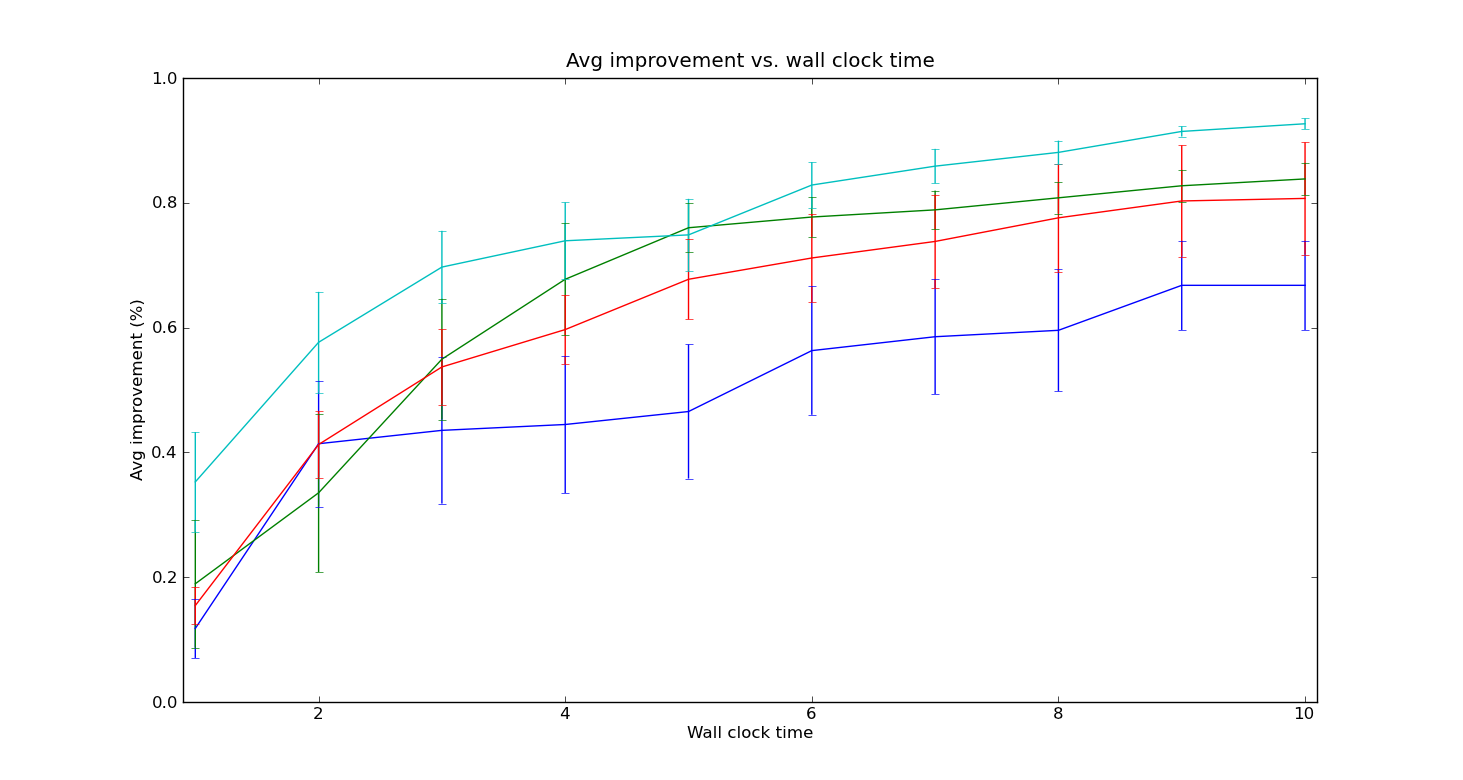
\includegraphics[width=\textwidth]{figures/EPI/speedup_vs_wallclock_8_core_9_its.png}}
    \caption[Parallel speedup for function drawn from prior]{Parallel speedup using function drawn from prior. We can see that the number of cores is directly related to the final average improvement. EPI with 8 cores results in a markedly better average improvement when compared to the serial method EGO (1 core).}
 	\label{fig:EPI_res1}
\end{figure}

%TODO
%Compare EPI to EI, constant liar and kriging believer

%\section{Speedup for large space}

%TODO
%if domain of sampling is large (ie $D >> l$) how does EPI compare to regular EI and random sampling
%\begin{figure}[hpt]
% 	\centerline{
\includegraphics[width=0.5\textwidth]{figures/placeholder.jpg}}
%    \caption[EPI comparison for large domain]{EPI vs EGO for large domain...}
% 	\label{fig:EPI_res3}
%\end{figure}

%\subsection{Comparison to other methods}
%
%TODO
%Compare EPI to space (in timing and accuracy)
%\begin{figure}[hpt]
% 	\centerline{
\includegraphics[width=0.5\textwidth]{figures/placeholder.jpg}}
%    \caption[EPI vs SPACE for large domain]{EPI vs SPACE for large domain...}
% 	\label{fig:EPI_res4}
%\end{figure}
%
%\section{Speedup for Branin function}
%
%TODO
%show contour of log like WITH vectors
%\begin{figure}[hpt]
% 	\centerline{
\includegraphics[width=0.5\textwidth]{figures/placeholder.jpg}}
%    \caption[Parallel speedup using Branin function]{Parallel speedup using Branin function...}
% 	\label{fig:EPI_res5}
%\end{figure}
%
%TODO
%show contour of log like WITH vectors
%\begin{figure}[hpt]
% 	\centerline{
\includegraphics[width=0.5\textwidth]{figures/placeholder.jpg}}
%    \caption[Comparison using Branin function]{Comparison using Branin function...}
% 	\label{fig:EPI_res6}
%\end{figure}

% chapter EPI Results (end)

\chapter{EPI Implementation} % (fold)
\label{cha:EPI Implementation}

\section{Adaptation of hyperparameters} % (fold)
\label{sec:Adaptation of hyperparameters}

In this section we show how we adapt the hyperparameters of the GP using the sampling information. This follows the methods outlined in \cite{RW}.

The log-likelihood of the data $\vec{y}$ given the points sampled $X$ and the hyperparameters $\theta$ is
\begin{equation}
    \log p(\vec{y}|X, \theta) = -\frac{1}{2}\vec{y}^{T}\Sigma^{-1}\vec{y} - \frac{1}{2}\log|\Sigma| - \frac{n}{2} \log 2\pi
\end{equation}
where $\Sigma$ is the covariance function defined as before, $\theta$ are the hyperparameters of the covariance function and $|\cdot|$ is the matrix norm defined for a matrix $B$ as
\begin{equation}
    |B| = \max \left( \frac{|B\vec{x}|}{|\vec{x}|} : \vec{x} \in \mathbb{R}^{n}\backslash\{\vec{0}\} \right).
\end{equation}

The partial derivative with respect to each hyperparameter $\theta_{i}$ is
\begin{equation}
    \frac{\partial}{\partial \theta_{i}} \log p(\vec{y}|X,\theta) = \frac{1}{2}\vec{y}^{T}\Sigma^{-1}\frac{\partial \Sigma}{\partial \theta_{i}} \Sigma^{-1}\vec{y} - \frac{1}{2} {\rm tr}\left( \Sigma^{-1}\frac{\partial \Sigma}{\partial \theta_{i}} \right)
\end{equation}
where tr$(\cdot)$ is the trace of a matrix. If we set $\vec{\alpha} = \Sigma^{-1}\vec{y}$ this further reduces to
\begin{equation}
    \frac{\partial}{\partial \theta_{i}} \log p(\vec{y}|X,\theta) = \frac{1}{2} {\rm tr}\left((\vec{\alpha}\vec{\alpha}^{T} - \Sigma^{-1})\frac{\partial \Sigma}{\partial \theta_{i}}\right).
\end{equation}

The key part of this equation is the partial derivative of $\Sigma$ with respect to each hyperparameter. For our squared exponential covariance function the partial derivatives are
\begin{equation}
    \frac{\partial}{\partial \sigma_{f}^{2}} \Sigma(x_{i}, x_{j}) = \exp\left( -\frac{1}{2l^{2}} |x_{i} - x_{j}|^{2}\right) = \frac{\Sigma(x_{i}, x_{j})}{\sigma_{f}^{2}},
\end{equation}
\begin{equation}
    \frac{\partial}{\partial l} \Sigma(x_{i}, x_{j}) = \frac{1}{l^{3}}|x_{i} - x_{j}|^{2}\Sigma(x_{i}, x_{j})
\end{equation}
and
\begin{equation}
    \frac{\partial}{\partial \sigma_{n}^{2}} \Sigma(x_{i}, x_{j}) = \delta_{ij}.
\end{equation}

\subsection{Example of hyperparameter evolution}

In this section we demonstrate the hyperparameter evolution capabilities of the software package. We start with a function drawn from the prior with hyperparameters set to $(\sigma_{f}^{2} = 1, l = 1, \sigma_{n}^{2} = 0.01)$ and a domain of $[-7,7]$. We set the initial hyperparameters at $(\sigma_{f}^{2} = 1, l = 2, \sigma_{n}^{2} = 0.1)$. As we sample points from the function we expect these hyperparameters to become closer and closer to those of the prior from which it was drawn.

As we sample sets of 20 points from a latin hypercube we notice in Figure \ref{fig:EPI_hyper_1} and Figure \ref{fig:EPI_hyper_2} that the likelihood of the parameters becomes maximized near the correct values. The algorithm is able to use gradient decent to find the point of maximum likelihood, the correct values of the hyperparameters.

\begin{figure}[hpt]
 	\centerline{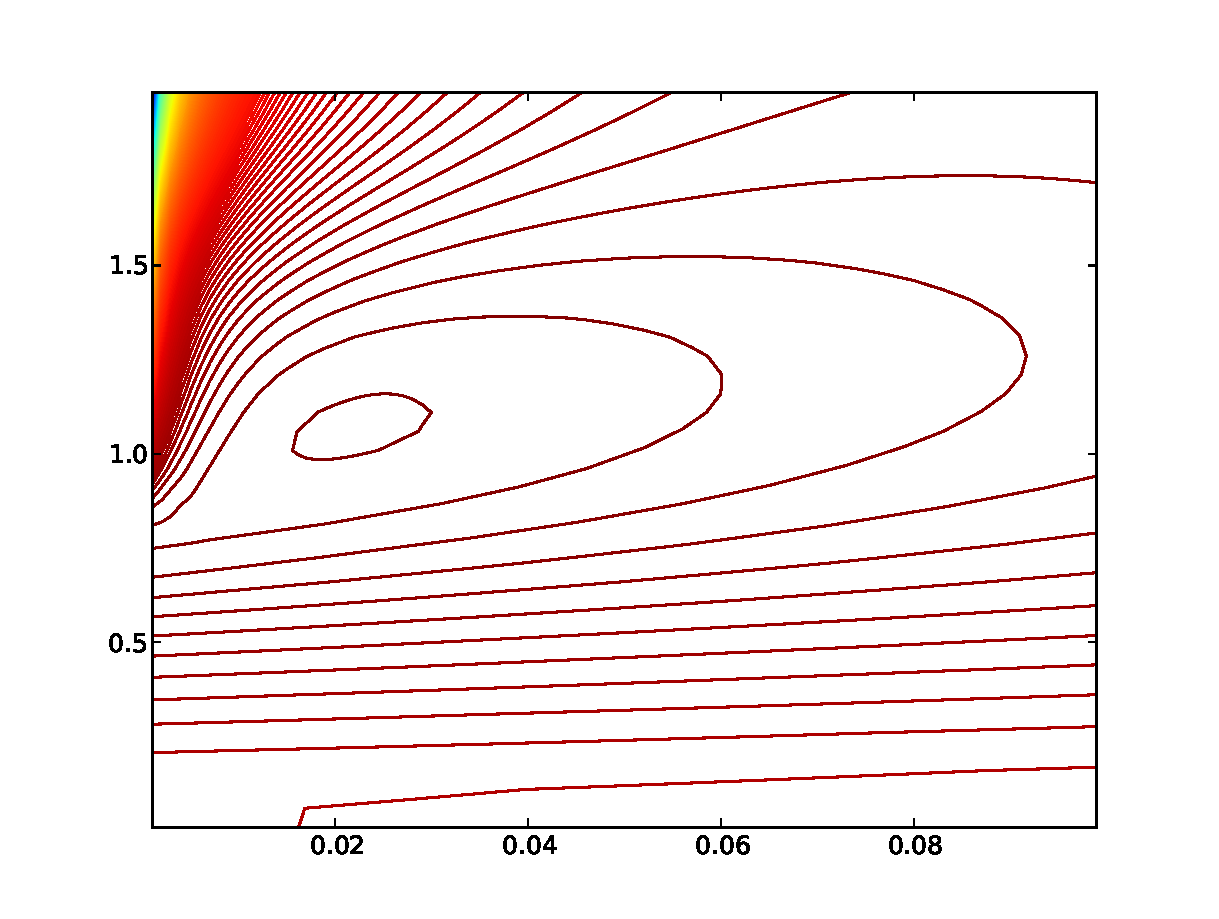
\includegraphics[width=.85\textwidth]{figures/EPI/hyper_update_loglike_20s.pdf}}
    \centerline{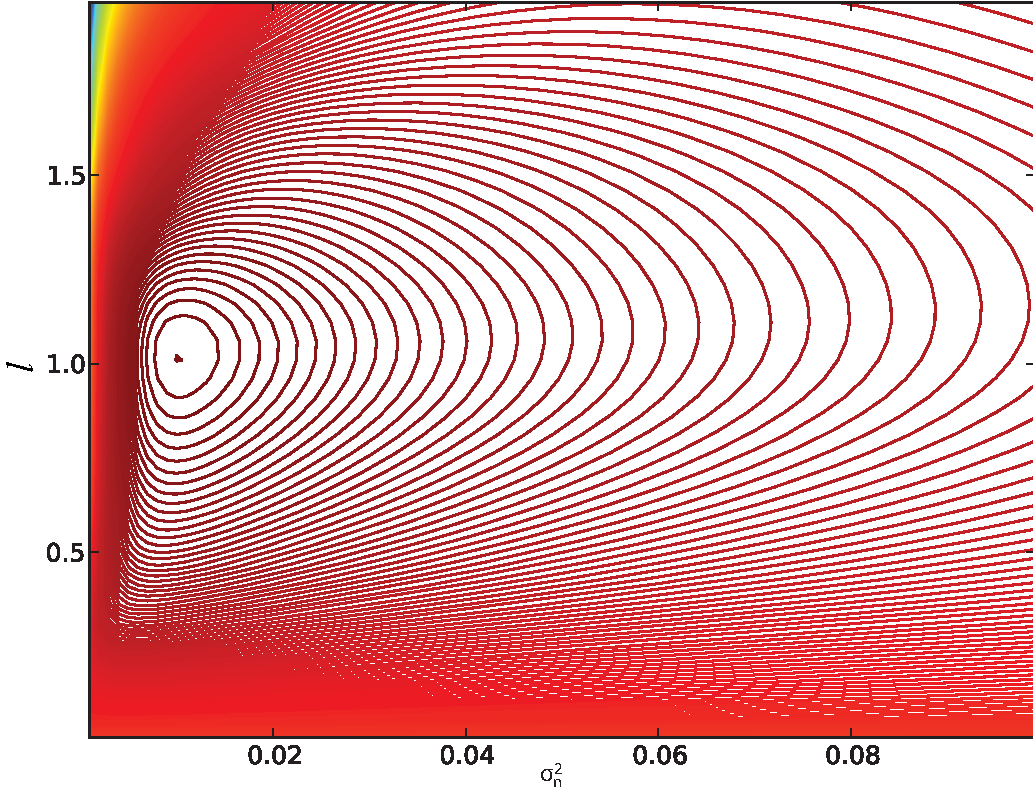
\includegraphics[width=.85\textwidth]{figures/EPI/hyper_update_loglike_60s.pdf}}
    \caption[Likelihood of hyperparameters]{Likelihood of hyperparameters $l$ and $\sigma_{n}^{2}$ at various values after 20 points (top) and 60 points (bottom) have been sampled from the function.}
 	\label{fig:EPI_hyper_1}
\end{figure}

\begin{figure}[hpt]
 	\centerline{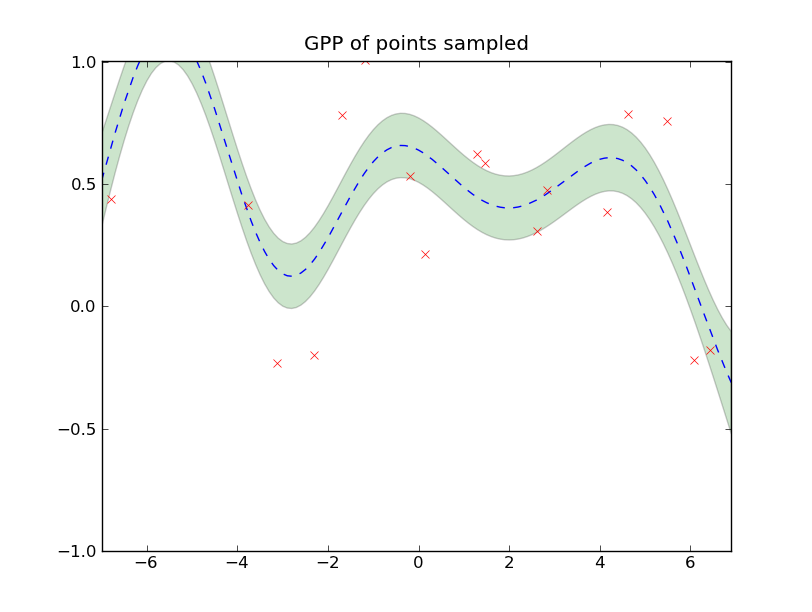
\includegraphics[width=0.75\textwidth]{figures/EPI/hyper_update_GPP_pre.png}}
    \centerline{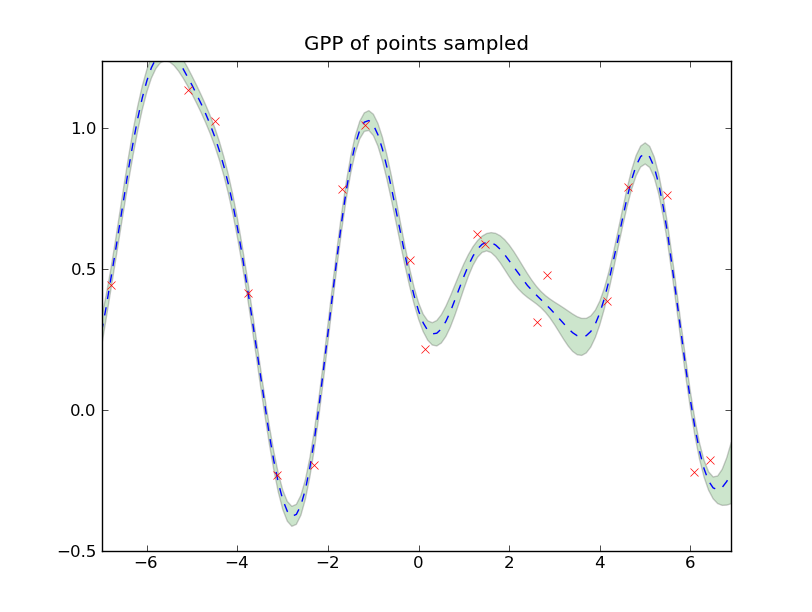
\includegraphics[width=0.75\textwidth]{figures/EPI/hyper_update_GPP_post.png}}
    \caption[Evolution of hyperparameters]{We note that visually the set of hyperparameters that the algorithm finds using the adaptive method provide a better fit to the data (bottom) than those initially provided in the experiment (top).}
 	\label{fig:EPI_hyper_2}
\end{figure}

% section Adaptation of hyperparameters (end)

\section{Math Appendix}

In this section we will show the component-wise calculation of the gradient of the covariance matrix as well as a method for differentiating the Cholesky decomposition of this matrix.

\subsection{Variance matrix calculations}
\label{EPI_imp_var}

From \cite{RW} we have
\begin{equation}
 \Sigma = K(\vec{x_{\star}}, \vec{x_{\star}}) - K(\vec{x_{\star}}, \vec{X}) K(\vec{X}, \vec{X})^{-1} K(\vec{X}, \vec{x_{\star}}).
\end{equation}
We will use $K^{-1} = K(\vec{X}, \vec{X})^{-1}$. We have by definition
\begin{equation}
 K(\vec{x_{\star}}, \vec{x_{\star}})_{ij} = K(x_{\star i}, x_{\star j})
\end{equation}
\begin{equation}
 K(\vec{x_{\star}}, \vec{X})_{ij} = K(x_{\star i}, X_{j})
\end{equation}
\begin{equation}
 K(\vec{X}, \vec{x_{\star}})_{ij} = K(X_{i}, x_{\star j}).
\end{equation}
We will define a temporary matrix $T^{(1)}$ to be
\begin{equation}
 T^{(1)} = K(\vec{x_{\star}}, \vec{X}) K^{-1}
\end{equation}
and decompose it into its components to get
\begin{equation}
 T^{(1)}_{ip} = \sum_{q = 1}^{N} K^{-1}_{qp} K(x_{\star i}, X_{q}).
\end{equation}
We then define
\begin{equation}
 T^{(2)} = T^{(1)} K(\vec{X}, \vec{x_{\star}})
\end{equation}
and decompose it to get
\begin{equation}
 T^{(2)}_{ij} = \sum_{p = 1}^{N} T^{(1)}_{ip} K(X_{p}, x_{\star j}) = \sum_{p = 1}^{N} \sum_{q = 1}^{N} K^{-1}_{qp} K(x_{\star i}, X_{q}) K(x_{\star j}, X_{p}).
\end{equation}
and note
\begin{equation}
 \Sigma_{ij} = K(\vec{x_{\star}}, \vec{x_{\star}})_{ij} - T^{(2)}_{ij}
\end{equation}
\begin{equation}
 \Sigma_{ij} = K(x_{\star i}, x_{\star j}) - \sum_{p = 1}^{N} \sum_{q = 1}^{N} K^{-1}_{qp} K(x_{\star i}, X_{q}) K(x_{\star j}, X_{p}).
\end{equation}
The partial derivative is found by applying the operation component wise and a simple use of the chain rule
\begin{equation}
 \begin{tabular}{rl}
 $\frac{\partial}{\partial x_{\star t}} \Sigma_{ij} =$ & $\frac{\partial}{\partial x_{\star t}} K(x_{\star i}, x_{\star j})$ \\
 & $- \sum_{p = 1}^{N} \sum_{q = 1}^{N} K^{-1}_{qp} \left( K(x_{\star i}, X_{q}) \frac{\partial}{\partial x_{\star t}} K(x_{\star j}, X_{p}) + K(x_{\star j}, X_{p}) \frac{\partial}{\partial x_{\star t}} K(x_{\star i}, X_{q}) \right)$
 \end{tabular}
\end{equation}
where we note that $\frac{\partial}{\partial x_{\star t}} T^{(2)}_{ij} = $
\begin{equation}
    \left\{ \begin{tabular}{cc}
        $2 \sum_{p = 1}^{N} \sum_{q = 1}^{N} K^{-1}_{qp} \left( K(x_{\star i}, X_{q}) \frac{\partial}{\partial x_{\star i}} K(x_{\star i}, X_{p}) \right)$ & $t = i = j$ \\
        $\sum_{p = 1}^{N} \sum_{q = 1}^{N} K^{-1}_{qp} K(x_{\star j}, X_{p}) \frac{\partial}{\partial x_{\star i}} K(x_{\star i}, X_{q})$ & $t = i \neq j$ \\
							$\sum_{p = 1}^{N} \sum_{q = 1}^{N} K^{-1}_{qp} K(x_{\star i}, X_{p}) \frac{\partial}{\partial x_{\star j}} K(x_{\star j}, X_{q})$ & $t = j \neq i$ \\
							$0$ & otherwise
                                                      \end{tabular} \right..
\end{equation}

\subsection{Differentiation of the Cholesky decomposition}

To incorporate the gradient into the Cholesky decomposition we follow the method outlined by \cite{Smith1995}.

The algorithm takes $\Sigma$ as input and produces a lower triangular matrix $L$ and $\frac{\partial}{\partial x_{\star t}} L$ such that $\Sigma = LL^{T}$.

We use the following notation
\begin{equation}
    \frac{\partial}{\partial x_{\star t}} L_{ij} = L_{ij} (x_{\star t})
\end{equation}
\begin{enumerate}
 \item $L_{ij} = \Sigma_{ij}$ \\
       $L_{ij (x_{\star t})} = \frac{\partial}{\partial x_{\star t}} \Sigma_{ij}$
 \item for $k = 1\ldots N$ if $|L_{kk}| > \epsilon_{m}$ (machine precision)
 \begin{enumerate}
  \item $L_{kk} = \sqrt{L_{kk}}$ \\
	$L_{kk (x_{\star t})} = \frac{1}{2} \frac{L_{kk (x_{\star t})}}{L_{kk}}$.
  \item for $j = k+1\ldots N$ \\
	$L_{jk} = L_{jk}/L_{kk}$ \\
	$L_{jk (x_{\star t})} = \frac{L_{jk (x_{\star t})} + L_{jk}L_{kk (x_{\star t})}}{L_{kk}}$.
  \item for $j = k+1\ldots N$ and $i = j\ldots N$ \\
	$L_{ij} = L_{ij} - L_{ik}L_{jk}$ \\
	$L_{ij (x_{\star t})} = L_{ij (x_{\star t})} - L_{ik (x_{\star t})}L_{jk} - L_{ik}L_{jk (x_{\star t})}$.
 \end{enumerate}

This returns a lower triangular matrix $L$ and $\frac{\partial}{\partial x_{\star t}} L$ such that $\Sigma = LL^{T}$.

\end{enumerate}

\section{GPGPU Computing} % (fold)
\label{sec:GPGPU Computing}

GPU computing allows for the cheap implementation of parallel algorithms. Modern graphics cards can have many hundreds of cores and can perform many teraFLOPS from within a desktop workstation. The development and maturation of C-like programing languages like CUDA and openCL allow for the implementation of parallel codes on these General Purpose Graphical Processing Units (GPGPUs) if the algorithm can be designed to fit into the tight memory restrictions of the GPGPU cores, as shown below.

\subsection{Expected Improvement}
\label{GPUEI}

The trivially parallelizeable Monte Carlo step in the expected improvement algorithm and relatively low memory requirements ($\mathcal{O}(l^{2})$) lends itself to GPGPU implementation perfectly. We implement this algorithm into a CUDA kernel and compare it to a serial python implementation.

%\subsubsection{Accuracy}
%
%When the dimension of the problem is low we can compute the expected improvement analytically. \cite{Ginsbourger2008} gives solutions for the 1-D and 2-D EI exactly. We compare our method to these and see how many MC iterations are required to achieve different levels of accuracy.
%
%TODO
%graph for 1 point, 2 points exp error vs analytic, var of error vs its

\subsubsection{Speedup}

The CUDA implementation of the EI algorithm is about 300 times faster to run on the GPGPU than on a CPU (using python). In figure \ref{GPUspeed1} we see the wall clock time required to compute the expected improvement for 4 points in 2 dimensions ($l=4, d=2$).

 \begin{figure}[hpt]
 	\centerline{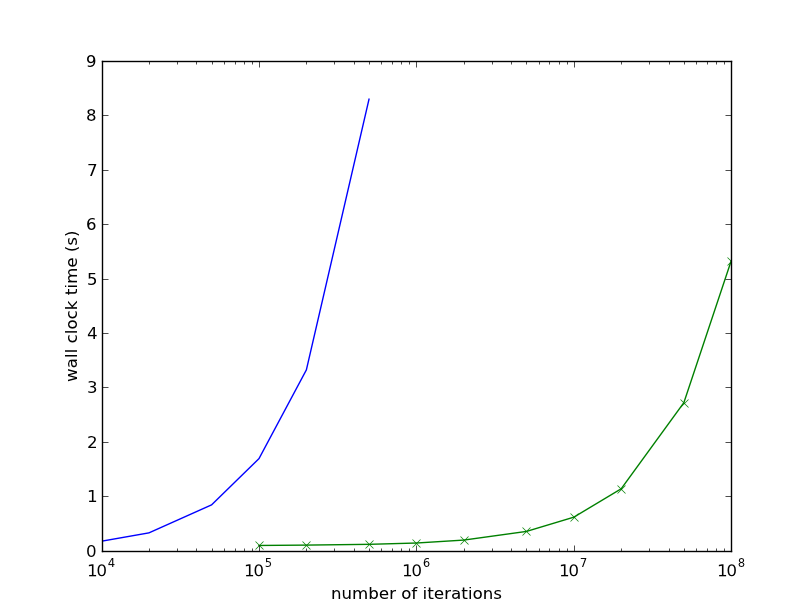
\includegraphics[width=\textwidth]{figures/EPI/exp_EI_speedup_vs_its.png}}
    \caption[CPU vs GPU time to compute EI]{Wall clock time to compute $\mathbb{E}_{n}\left[{\rm EI}(\vec{x})\right]$ on a CPU (blue, line) and GPU (green, x) for $l = 4$.}
 	\label{GPUspeed1}
 \end{figure}

%\subsection{Gradient of Expected Improvement}
%
%MC step, some memory problems (see section).
%
%TODO
%graph: wall clock time vs number of iterations
%graph: wall clock time vs number of samples
%graph: wall clock time vs number of restarts (paths)

\subsection{Memory Restrictions} % (fold)
\label{sub:Memory Restrictions}

GPGPU cores have very low memory per core/block (16KB for tesla, 4KB for a GT 2{\it XX} card). Our algorithm uses matrices of various sizes (table \ref{EPImemory}), some of which grow to be quite large as more points are sampled.

\begin{table}
    \caption{GPP matrix memory footprint}
    \label{EPImemory}
\begin{center}
    \begin{tabular}{c|c}
    Variable & Size \\
    \hline
    $K$ & $n \times n$ \\
    $K_{\star }$ & $n \times l$ \\
    $K_{\star \star }$ & $l \times l$ \\ 
    $L = {\rm cholesky}(K + \sigma^{2}I) $ & $n \times n$ \\
    $\vec{v} = L \backslash K_{\star }$ & $n \times l$ \\
    $\vec{\alpha} = L^{T} \backslash L \backslash \vec{y}$ & $n \times 1$ \\
    $\vec{\mu} = K_{\star }^{T}\vec{\alpha}$ & $l \times 1$  \\
    $\Sigma = K_{\star \star} - \vec{v}^{T}\vec{v}$ & $l \times l$ \\
    $\vec{\nabla} \vec{\mu}$ & $l \times d$ \\
    $\vec{\nabla} \Sigma$ & $l \times l \times d$
    \end{tabular}
\end{center}
\end{table}

The trivially MC portions of the algorithm only ``need" the matrices of size $l \times l$ to compute their estimates, so that is all that is sent to the GPU, the calculations involving $n \times n$ are computed on the CPU where system memory is abundant.

\subsubsection{Memory Transfer} % (fold)
\label{ssub:Memory Transfer}

The required vectors and matrices need to be transfered to the GPU as linear arrays. This is accomplished by flattening each component in the following ways. This allows for easy deconstruction into 2-D and 3-D arrays once the data is in the global memory of the GPU.

\begin{equation}
    \vec{\mu} = \left[ \underbrace{\left[ \underbrace{\left[\mu_{1}^{(1)}, \ldots, \mu_{c}^{(1)}, \mu_{c+1}^{(1)}, \ldots, \mu_{l}^{(1)} \right]}_{l}, \ldots, \underbrace{\left[\mu_{1}^{(R)}, \ldots, \mu_{c}^{(R)}, \mu_{c+1}^{(R)}, \ldots, \mu_{l}^{(R)} \right]}_{l} \right]}_{R} \right]
\end{equation}

Requiring memory of $O(lR)$ per run, $O(l)$ per GPU block.

\begin{equation}
    \Sigma = \left[ \underbrace{ \left[ \underbrace{ \left[ \underbrace{ \left[ \Sigma_{11}^{(1)}, \ldots, \Sigma_{1l}^{(1)} \right]}_{l}, \ldots, \underbrace{ \left[ \Sigma_{l1}^{(1)}, \ldots, \Sigma_{ll}^{(1)} \right]}_{l} \right] }_{l}, \ldots, \underbrace{ \left[ \underbrace{ \left[ \Sigma_{11}^{(R)}, \ldots, \Sigma_{1l}^{(R)} \right]}_{l}, \ldots, \underbrace{ \left[ \Sigma_{l1}^{(R)}, \ldots, \Sigma_{ll}^{(R)} \right]}_{l} \right] }_{l}  \right]}_{R}\right]
\end{equation}

Requiring memory of $O(l^{2}R)$ per run, $O(l^{2})$ per GPU block.

\begin{equation}
    \nabla \vec{\mu} = \left[ \underbrace{ \left[ \underbrace{ \left[ \underbrace{ \left[ \nabla_{\vec{x_{1}}} \mu_{1}^{(1)} \right]}_{d} , \ldots, \underbrace{ \left[ \nabla_{\vec{x_{l}}} \mu_{l}^{(1)} \right]}_{d}\right]}_{l}, \ldots, \underbrace{ \left[ \underbrace{ \left[ \nabla_{\vec{x_{1}}} \mu_{1}^{(R)} \right]}_{d} , \ldots, \underbrace{ \left[ \nabla_{\vec{x_{l}}} \mu_{l}^{(R)} \right]}_{d}\right]}_{l} \right]}_{R} \right]
\end{equation}

Requiring memory of $O(ldR)$ per run, $O(ld)$ per GPU block.

\begin{equation}
    \nabla \Sigma = \left[ \underbrace{ \left[ \underbrace{ \left[ \underbrace{ \left[ \underbrace{ \left[ \nabla_{\vec{x_{1}}} \Sigma_{11}^{(1)} \right]}_{d} , \ldots, \underbrace{ \left[ \nabla_{\vec{x_{l}}} \Sigma_{1l}^{(1)} \right]}_{d}\right]}_{l}, \ldots, \underbrace{ \left[ \underbrace{ \left[ \nabla_{\vec{x_{1}}} \Sigma_{l1}^{(1)} \right]}_{d} , \ldots, \underbrace{ \left[ \nabla_{\vec{x_{l}}} \Sigma_{ll}^{(1)} \right]}_{d}\right]}_{l} \right] }_{l}, \ldots \right]}_{R} \right]
\end{equation}

Requiring memory of $O(l^{2}dR)$ per run, $O(l^{2}d)$ per GPU block.

\begin{equation}
    \nabla {\rm EI} = \left[ \underbrace{ \left[ \underbrace{ \left[ \underbrace{ \left[ \nabla_{\vec{x_{1}}} {\rm EI}^{(1)} \right]}_{d} , \ldots, \underbrace{ \left[ \nabla_{\vec{x_{l}}} {\rm EI}^{(1)} \right]}_{d}\right]}_{l}, \ldots, \underbrace{ \left[ \underbrace{ \left[ \nabla_{\vec{x_{1}}} {\rm EI}^{(R)} \right]}_{d} , \ldots, \underbrace{ \left[ \nabla_{\vec{x_{l}}} {\rm EI}^{(R)} \right]}_{d}\right]}_{l} \right]}_{R} \right]\end{equation}

Requiring memory of $O(ldR)$ per run, $O(ld)$ per GPU block.

% subsubsection Memory Transfer (end)

% subsection Memory Restrictions (end)

% section GPGPU Computing (end)

\section{Availability and requirements}
 \begin{itemize}
  \item \textbf{Project name:} EPI
  \item \textbf{Project home page:} www.github.com/sc932/EPI
  \item \textbf{Operating systems:} Linux 32/64-bit, Mac OSX, Windows (Cygwin)
  \item \textbf{Programming languages:} Python, C, CUDA
  \item \textbf{Other requirements:} Some python packages, see documentation
  \item \textbf{License:} UoI/CNSA Open Source
 \end{itemize}


% chapter EPI Implementation (end)

% part EPI: Expected Parallel Improvement (end)

\part{Velvetrope} % (fold)
\label{prt:Velvetrope}
\singlespacing

\noindent
\Large
Velvetrope: a parallel, bitwise algorithm for finding homologous regions within sequences

\noindent
\normalsize
Joint work with Nick Hengartner$^{1}$ and Joel Berendzen$^{2}$ \\
\scriptsize
$^{1}$Information Sciences Group (CCS-3), MS B265, Los Alamos National
 Laboratory, Los Alamos, NM 87545, USA \\
$^{2}$Applied Modern Physics Group (P-21), MS D454, Los Alamos National
 Laboratory, Los Alamos, NM 87545, USA
\normalsize

\normalspacing

\begin{center}
   Abstract 
\end{center}

Existing methods for recognizing common patterns in sequence data
streams do not scale well. This scaling problem becomes critical for
problems that are driven by large-scale sequencing, such as
metagenomics and cancer genomics.  Restricting comparisons to exact
identities of amino acids between a single test sequence and a set of
test sequences allows many efficiencies to be realized, including
bitwise parallel operation and low-order scaling.

We introduce an algorithm based on global and local densities of
matches at the amino-acid level that finds areas of high commonality
across a set of sequences.  It produces results that are intermediate
between local and multiple sequence alignment and can address
questions that other approaches cannot.  The speed of the
algorithm is superior to BLASTX and HMMER v3, and the scaling is
$\mathcal{O}$($N$) where $N$ is the total length of the sequences
being compared.

\chapter{Velvetrope Introduction} % (fold)
\label{cha:Velvetrope Introduction}
\noindent
Next generation biological sequencing technologies have created a virtual torrent of new sequence data. The analysis challenges that this data presents need to be addressed by new algorithms that are designed to be as efficient as possible and can scale with the data. One area of analytic interest is that of alignment, finding where two genetic sequences are similar. Finding these highly conserved regions can lead to new insights on how distantly related organisms perform related tasks. By examining all of the ways that nature has evolved solutions to a specific challenge, like synthesizing glucose, we can come up with new and efficient techniques for applications in everything from biofuels to medicine.

Finding shared elements of sequence among possibly-related genes is a
fundamental operation that underlies most of the analytical methods of
molecular biology, including local sequence alignment, gene matching,
multiple sequence alignment, phylogenetic tree calculation, and
taxonomic assignments. The earliest approaches to finding this homology
between sequences was derived from pairwise sequence alignment algorithms
such as Needleman-Wunsch \cite{Needleman70} or Smith-Waterman
\cite{SmithWaterman} both of which employ dynamic programming and
are computationally expensive, in the sense that it does not scale linearly with the size of the data. A second approach employs
hidden--Markov model (HMM) algorithms such as HMMer
\cite{Eddy98}. The HMM may be local or non-local in nature, is
built up by training from a curated data set, and is also generally
computationally expensive. A third approach relies upon exact or
near-exact matches between short solid patterns ($k$-mers for a length $k$) before also resorting to dynamic programming.  The
$k$-mer approach underlies many algorithms such as the widely--used
pairwise aligner and gene matcher BLAST \cite{BLAST} and its
relatives \cite{BLAT,Megablast,PSIBLAST}. $k$-mers also are the first pass in the widely used multiple--sequence aligners
MUSCLE \cite{MUSCLE} and DIALIGN-TX \cite{DIALIGN-TX}. Though the $k$-mer approach can be made quite computationally
efficient, especially as $k$ is made large, detecting distant
homologies requires use of short values of $k$ and it is easy to
construct pathological cases where commonality will not be detected
even for the limiting value of $k = 1$.

The importance of computational efficiency and scaling is made paramount by the recent advances
and demands of data-driven projects in fields such as
shotgun metagenomic sequencing and cancer genomics. Such projects
routinely create data sets exceeding 10 Gbp ($10^{10}$bp) and will soon extend
to the Tbp ($10^{12}$bp) region as new sequencing technologies come online. Speed
and scaling, especially at the early steps of analysis, is critical to make advances in these fields tractable.

Velvetrope was conceived to enable the identification of sequence homology with an algorithm that
is simple, scalable and parallel from the start. Our approach is based on finding areas of high densities of shared identities (Amino Acid or DNA) in local
(adjustable) regions between sequences, rather than finding $k$-mers. This allows for rapid bitwise operations between sequences, computeable in parallel. These areas are found by performing first a global, then local filter on the shared identities. By omitting the $k$-mer step we allow Velvetrope to access homology information between evolutionarily distant sequences otherwise inaccessible by other existing methods.

While areas of high sequence identity density are qualitatively similar to local alignments, they are significantly different from the outputs of traditional pairwise-local or global alignment algorithms. These regions do correspond to areas with a high probability of being in a standard alignment as they represent areas of high local homology. Rather than explicitly calling these regions alignments we refer to them as ``in the club,'' thus giving rise to the name, 'Velvetrope' the traditional barrier between those in and out of a club.

Velvetrope is a quick, simple and highly parallelizable method (we present both a serial and parallel implementation)
that finds areas of high similarity between many
sequences in a pairwise fashion, never performing a $k$-mer based step and independent of order. This allows for it
to quickly find areas of high local homology, including areas that these other
methods may ignore like proteins with transposed domains.

% chapter Velvetrope Introduction (end)

\chapter{Velvetrope Methods} % (fold)
\label{cha:Velvetrope Methods}

To find the areas of high local homology between sequences we employ a two-part filtering system that first finds offsets (sets of positions) where two sequences share a higher than expected amount of identity (global filter), and then filters these sets of positions to find areas with higher than expected identity within them (local filter).

Velvetrope's filtering system implements only bitwise operations on a sequence of interest $S$ compared against a possibly large set of other test sequences \textbf{T}. The first step is a global filter and works by taking the sequence of interest and comparing it using DNA or Amino Acid translations (up to 6 frames of reference). For the motivating examples we will assume we are in a coding region and use an Amino Acid translation. We can compare the sequence $S$ against each sequence in the set of sequences to be compared against $T \in$ \textbf{T}  using simple AND operations. To track the sequence identities within these offsets we construct a binary concordance matrix $M$ that keeps track of all matches (sequence identities) across all possible offsets between the two sequences.

The aggregate number of matches for every offset found is compared to what would be expected if the test sequence were randomly rearranged at that offset; if the number of matches is above some threshold then this offset is saved as having a possible area of high local homology; this is the global filter. All possible offsets up to the length of the proposed sequence are checked in this fashion. By looking at all possible offsets between the two sequences we can allow the areas being compared to shift across the two sequences, even becoming transposed if need be. This can be done in parallel for all sequences in \textbf{T} and even across different offset sets within a particular test sequence.

The next filter is local and works by looking over a fixed-bit window in each of the possible offsets proposed by the first step. The window keeps a running average of the number of matches within it, correcting for the expected number of random matches and keeping track of only the difference between the number of matches were actually found and what is expected. When there is a large spike in this value then the window has shifted over an area with a large number of possibly non-random matches, an area of high sequence identity density. The region is then saved as an area of high local homology between the two sequences.

\section{Construction of the Concordance Matrix $M$}

We construct the concordance matrix $M$ by comparing a sequence of interest $S$ against each test sequence $T \in$ \textbf{T} aligned so residue 1 in the sequence of interest ($S_{1}$) is being compared to residue 1 of the test sequence ($T_{1}$), residue 2 compared against residue 2 ($S_{2},T_{2}$), etc. The first row of the bit-matrix is then constructed as follows: if the residue in the sequence of interest matches the residue it is lined up against in the test sequence then we give that position a value of 1, otherwise we give it a 0. We note that the row has length $\min(L_{S},L_{T})$, where $L_{S}$ is the length of the sequence of interest $S$ and $L_{T}$ is the length of the test sequence $T$. The test sequence is then shifted so that now residue 2 of the test sequence ($T_{2}$) lines up with residue 1 of the sequence of interest ($S_{1}$), residue 3 compared against residue 2 etc. ($T_{3},S_{2}$). This corresponds to offset 2. The second row is then constructed as before. We define some minimum window size $w$ (user defined, initialized to 20), all $L_{S} + L_{T}-2w$ possible offsets of overlap greater than or equal to $w$ are tested. In general
\begin{equation}
    M_{ij} = \left\{\begin{tabular}{cc} 1 & if $S_{j} = T_{i+j}$ \\ 0 & otherwise \end{tabular}\right.,
\end{equation}
for all
\begin{equation}
    1 \leq i \leq L_{S} + L_{T}-2w
\end{equation}
and
\begin{equation}
    \max(1,L_{T} - (w+i)) \leq j \leq \max(1,i+w-L_{S}).
\end{equation}
This creates a banded $(L_{S} + L_{T}-2w) \times (\min(L_{S},L_{T}))$ matrix $M$ that contains all pairwise comparisons between all possible offsets of size at least $w$ between the sequence of interest $S$ and the test sequence $T$. Instead of using the binary matrix we could also use a transition matrix such as the BLOSSUM62 matrix \cite{Henikoff1992} to encode more information about the relative similarity of individual amino acids at the cost of higher memory requirements (which is highly restricted in GPGPUs).

If every amino acid in $T$ were randomly distributed and there were equal frequencies of every amino acid we would have (inside the band of the matrix that actually contains information)
\begin{equation}
    E[M_{ij}] = \frac{1}{20}.
\end{equation}
This is not always true, and the algorithm takes local expectation into account, but this can be used as an approximation for motivation purposes. This is to say, long linear stretches of ones in this matrix should be rare and possibly contain useful information about areas of high similarity.

For example purposes we will compare the RNA Polymerase Beta Subunit between {\it E. Coli} and {\it Bacillus subtilis} \cite{GenBank} for the rest of the implementation section. We can see the row sum of the concordance matrix that these two genes imply compared against the expectation in Table \ref{VRtab1} and \ref{VRtab2}.

\begin{table}[htp]
    
    \label{VRtab1}
\begin{center}
{\small
\begin{tabular}{|ccccccccccc|}                                                                                                     
\hline                                                                                                                                      
\scriptsize{residue} & \small{1181} &  \small{1182} &  \small{1183} &  \small{1184} &  \small{1185} &  \small{1186} &  \small{1187} &  \small{1188} &  \small{1189} & \small{}$\cdots$ \\                                                                                             
SOI & \textcolor{blue}{I} &  \textcolor{blue}{A} &  \textcolor{blue}{T} &  \textcolor{blue}{P} &  \textcolor{blue}{V} &  \textcolor{blue}{F} &  \textcolor{blue}{D} &  \textcolor{blue}{G} &  \textcolor{blue}{A} & $\cdots$ \\                                                                                                                                                                                
\hline                                                                                                                                                                                                      
\scriptsize{offset} & $\vdots$ &  $\vdots$ &  $\vdots$ & $\vdots$ &  $\vdots$ &  $\vdots$ & $\vdots$ &  $\vdots$ &  $\vdots$ & \\                                                                                                                                                                          
\small{971}$\cdots$ & * & * & * & I & H & I & A & S & P & $\cdots$ \\                                                                                  
\small{972}$\cdots$ & * & * & I & H & I & A & S & P & V & $\cdots$ \\                                                                                  
\small{973}$\cdots$ & * & I & H & I & A & S & P & V & F & $\cdots$ \\                                                                                  
\small{974}$\cdots$ & \textcolor{red}{I} & H & I & A & S & P & V & F & D & $\cdots$ \\                                                                 
\small{975}$\cdots$ & H & I & A & S & P & V & F & D & G & $\cdots$ \\
\small{976}$\cdots$ & \textcolor{red}{I} & \textcolor{red}{A} & S & \textcolor{red}{P} & \textcolor{red}{V} & \textcolor{red}{F} & \textcolor{red}{D} & \textcolor{red}{G} & \textcolor{red}{A} &  $\cdots$ \\
\small{977}$\cdots$ & A & S & P & V & F & D & G & A & R & $\cdots$ \\
\small{978}$\cdots$ & S & P & V & F & D & G & A & R & * & $\cdots$ \\
\small{979}$\cdots$ & P & V & F & D & G & A & R & * & * & $\cdots$ \\
\small{980}$\cdots$ & V & F & D & G & A & R & * & * & * & $\cdots$ \\
 & $\vdots$ &  $\vdots$ &  $\vdots$ &  $\vdots$ & $\vdots$ &  $\vdots$ &  $\vdots$ &  $\vdots$&  $\vdots$ & \\
\hline
\end{tabular}
}
\end{center}
\caption[Velvetrope offset matrix]{This is a subset of the 'offset matrix' constructed when comparing two genes. The black letters represent residues 1181-1189 of our sequence of interest. We are looking at a small section of the rows represented by offsets of 971-980. A red letter represents a match. As we can see there is an area of possible alignment in offset 976 as there are many more matches than we would believe to be expected.}
\end{table}

\begin{table}[htp]
    
    \label{VRtab2}
\begin{center}
{\small
\begin{tabular}{|ccccccccccc|}                                                                                                     
\hline                                                                                                                                      
\scriptsize{residue} & \small{1181} &  \small{1182} &  \small{1183} &  \small{1184} &  \small{1185} &  \small{1186} &  \small{1187} &  \small{1188} &  \small{1189} & \small{}$\cdots$ \\                                                                                             
\hline                                                                                                                                                                                                      
\scriptsize{offset} & $\vdots$ &  $\vdots$ &  $\vdots$ & $\vdots$ &  $\vdots$ &  $\vdots$ & $\vdots$ &  $\vdots$ &  $\vdots$ & \\                                                                                                                                                                          
\small{971}$\cdots$ & * & * & * & 0 & 0 & 0 & 0 & 0 & 0 & $\cdots$ \\                                                                                  
\small{972}$\cdots$ & * & * & 0 & 0 & 0 & 0 & 0 & 0 & 0 & $\cdots$ \\                                                                                  
\small{973}$\cdots$ & * & 0 & 0 & 0 & 0 & 0 & 0 & 0 & 0 & $\cdots$ \\                                                                                  
\small{974}$\cdots$ & \textcolor{red}{1} & 0 & 0 & 0 & 0 & 0 & 0 & 0 & 0 & $\cdots$ \\                                                                 
\small{975}$\cdots$ & 0 & 0 & 0 & 0 & 0 & 0 & 0 & 0 & 0 & $\cdots$ \\
\small{976}$\cdots$ & \textcolor{red}{1} & \textcolor{red}{1} & 0 & \textcolor{red}{1} & \textcolor{red}{1} & \textcolor{red}{1} & \textcolor{red}{1} & \textcolor{red}{1} & \textcolor{red}{1} &  $\cdots$ \\
\small{977}$\cdots$ & 0 & 0 & 0 & 0 & 0 & 0 & 0 & 0 & 0 & $\cdots$ \\
\small{978}$\cdots$ & 0 & 0 & 0 & 0 & 0 & 0 & 0 & 0 & * & $\cdots$ \\
\small{979}$\cdots$ & 0 & 0 & 0 & 0 & 0 & 0 & 0 & * & * & $\cdots$ \\
\small{980}$\cdots$ & 0 & 0 & 0 & 0 & 0 & 0 & * & * & * & $\cdots$ \\
 & $\vdots$ &  $\vdots$ &  $\vdots$ &  $\vdots$ & $\vdots$ &  $\vdots$ &  $\vdots$ &  $\vdots$&  $\vdots$ & \\
\hline
\end{tabular}
}
\end{center}
\caption[Velvetrope offset bit-matrix]{The matches of the offset matrix encoded into a binary bit-matrix. A 1 represents a match, a 0 represents no match. Alternatively a BLOSSUM or other amino acid transition matrix could be used in lieu of the more simple (and less memory intensive) bit matrix shown.}
\end{table}

\section{First filter: Global}

Now that we have this $(L_{S} + L_{T}-2w) \times (\min(L_{S},L_{T}))$ binary matrix $M$, we want to find what offsets result in abnormal quantities of matches. We want to find the rows in the matrix that have a higher than expected number of ones in them. To do this we take the sum of each row and compare it to the expectation of the number of matches based on amino acid frequency between that offset of the test sequence and the sequence of interest using a random model. If the sum of the ones is higher than some predetermined multiple of standard deviations away from the mean then it is marked as having a possible alignment. A default value of 3.5 assures that false positives should be extremely rare. We mark a row $i$ if,
\begin{equation}
    \sum_{j} M_{ij} > E\left(\sum_{j} A_{ij}\right) + \alpha \sqrt{E\left(\sum_{j} A_{ij}\right)}.
\end{equation}
where $E(X)$ is the expectation of $X$, $A_{i:}$ is a random vector constructed from sequences with the same amino acid composition, $\alpha$ is a parameter and is set to 3.5 by default and the square root represents the standard deviation (we assume a Poisson distribution). The value of 3.5 ensures a false positive rate of less than 0.1\% and we only look at one side distribution, offsets with higher than expected matches. The value of the mean and expectation is calculated analytically by combinatorially looking at all possible permutations of the test sequence. See figure \ref{fig:vr01}.

We note that as the lengths of the sequences grow large the signal can become lost in the noise. Even a $k$-mer of length 1Kbp would be lost when comparing a 3Gbp sequence using this method. To account for this and also to make easier use of the Graphics Processing Unit (GPU) implementation of this algorithm, which enforces strict memory constraints, we break up the sequences into chunks of length 1000 before forming the matrix $M$. This not only ensures that the noise will not overwhelm the signal, but also allows for much faster, parallel implementations. Areas of similarity that extend over a separation are rejoined in the recompilation step. By only looking over a linear number of offsets in the length of the test sequences we achieve scaling of
$\mathcal O$($N$) where $N$ is the total length of the sequences
being compared. This is far less computationally complex than the alternative dynamic programming and HMM based methods.

 \begin{figure}[htp]%figure2
 \centerline{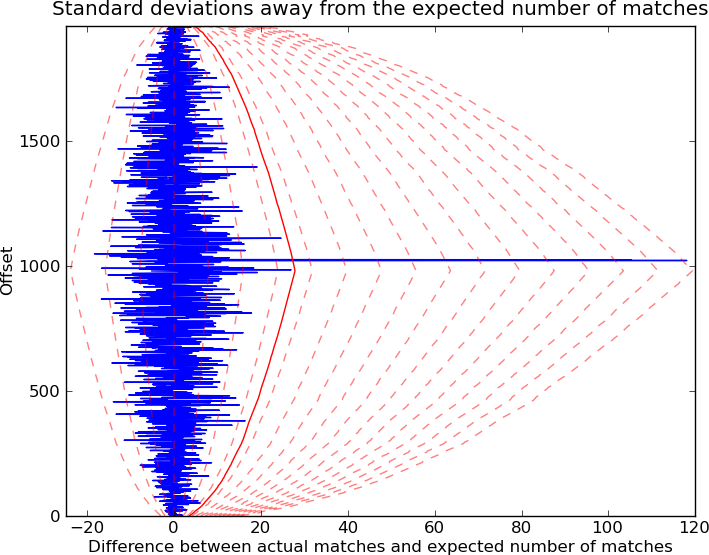
\includegraphics[width=\textwidth]{figures/velvetrope/globalFilterDuo.png}}
 \caption[First Velvetrope filter]{Values of sums of rows of the bit matrix plotted against standard deviations from the mean. The right picture is a zoom in of the area where all 4 qualifying offsets lie.}
 	\label{fig:vr01}
 \end{figure}

\section{Second filter: Local}

We now have the set of offsets that have a significant number of ones in them. The next goal is to quickly find where the areas of high density are in these vectors, if such areas exist, as these would be areas of high homology between the sequences. This is done by taking a running sum of each vector from its start; at each point we subtract off the expectation based on the amino acid frequency of the two sequences for each position. This has an effect of calculating how many ones have been found at or before that position above the number that would be expected. We know that this value must increase at some point in the vector because at the end there needs to be some extra number of ones equal to some number of standard deviations away from the mean, based on it passing the global step. Where this value peaks is where the club starts (it has a significant jump in the running sum over some window). When the value flattens out again that part of the sequence is no longer in the club (see Figure \ref{fig:vr02}).

Two parameters are used here (combined with the one from the global filter, they represent all three parameters of the model), the width of the block used for approximating the derivative and the number of matches above the expectation that are needed to trigger the start of the region. We can get the quick, bitwise location of the high density region in the vector, which corresponds to our ``in the club" region. A useful side effect of this filter is that if there is no region of high density, if we have just accidentally found an outlier from the global filter that just happens to have a lot of sparse matches, then it will not trigger and we will not get a false positive from the result of the global step.

 \begin{figure}[htp]%figure3
 \centerline{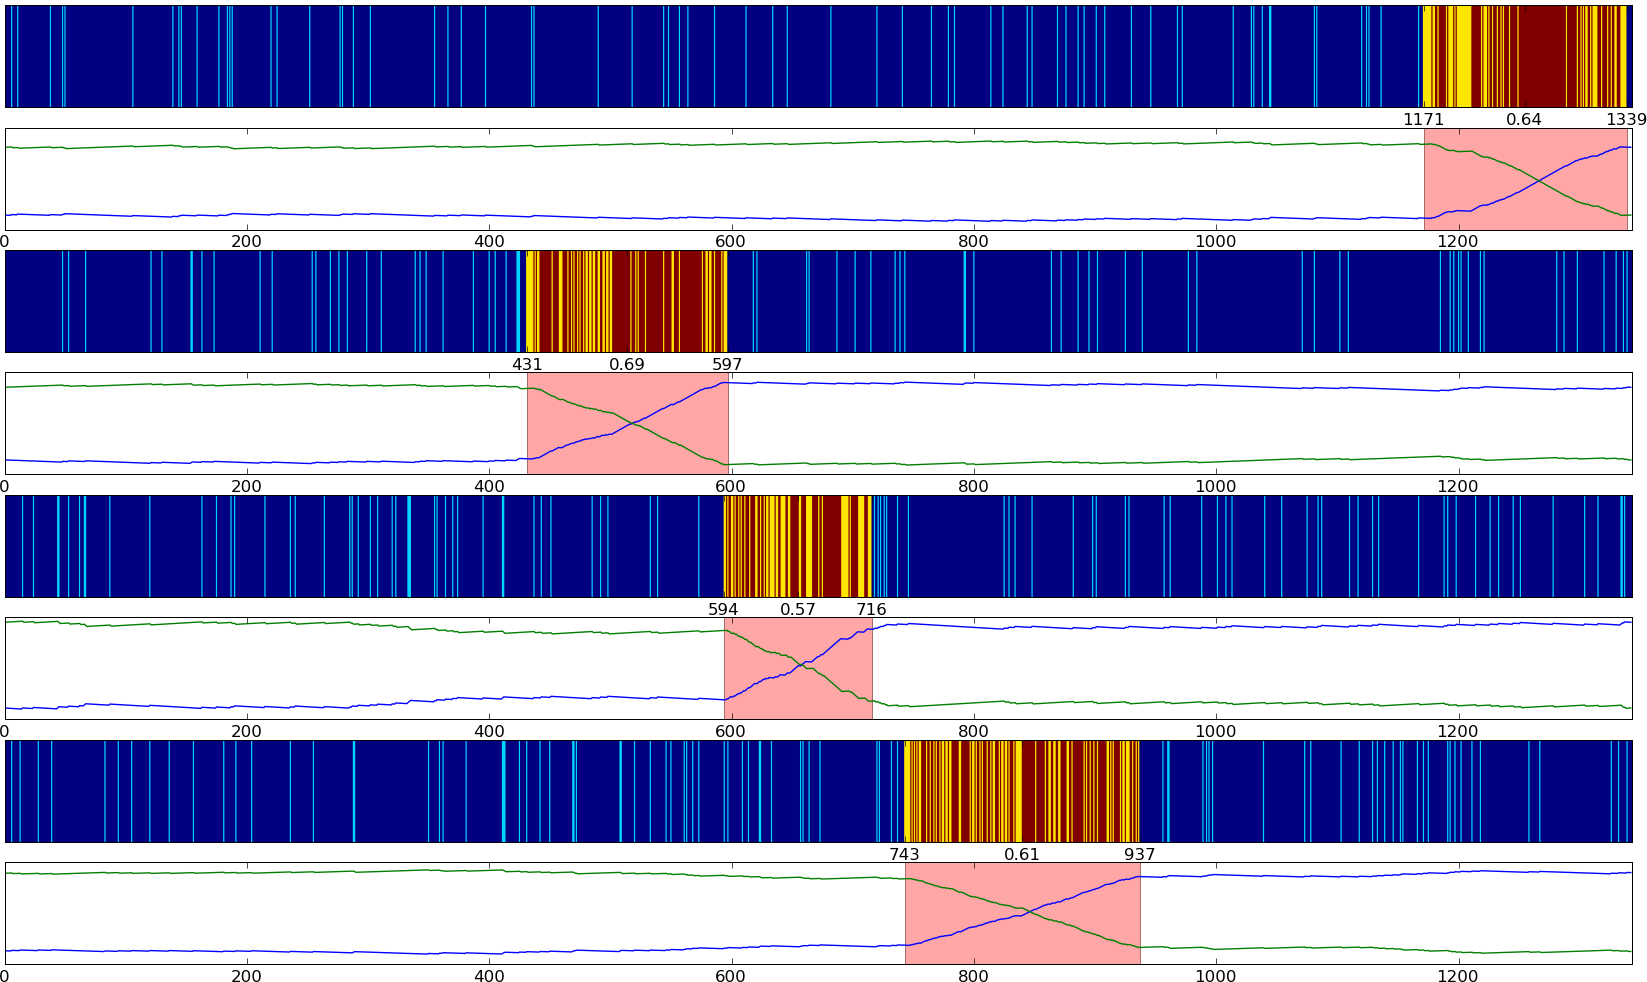
\includegraphics[width=\textwidth]{figures/velvetrope/localAlignmentsCDF.png}}
 \caption[Second Velvetrope filter]{The four vectors that passed the global filter test and their running sum calculation. When the approximate derivative of the running sum reaches a certain point the region is marked as having a possible alignment and shaded. For the vector blue means no match and not in that region, cyan is a match but not in the region (random match), yellow is the region of possible alignment and red are the positions in that region that have matches. The location of the region is marked along with the total density of matches within that region.}
 	\label{fig:vr02}
 \end{figure}

\section{Recompilation}

Now we have identified the regions where we have reason to believe there are local alignments between the two sequences, our ``in club" areas. We can see where they lie on their respective sequences and how their densities compare with each other and the sequences as a whole. This can be important information because the shifting of conserved regions and possible transposition events can represent evolutionary distance between the sequences. If we consider the conserved regions to be fixed by natural selection, then their relative drift away from each other should be related to the point when they originally diverged. We can see an example of this in Figure \ref{fig:vr03} where there is a difference in the sequence length between conserved areas of sequence.

 \begin{figure}[htp]%figure4
 \centerline{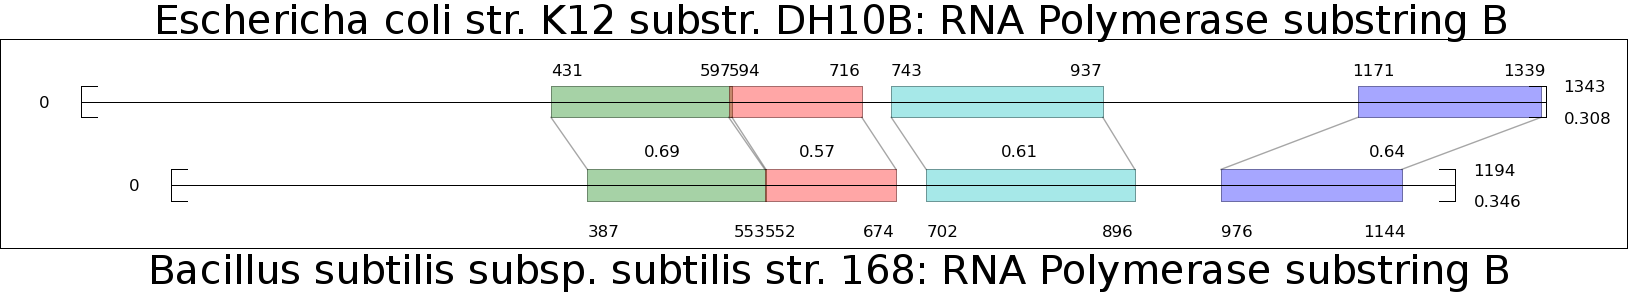
\includegraphics[width=\textwidth]{figures/velvetrope/localAlignmentsBreakout.png}}
 \caption[Local alignments]{Above we see where each area of possible local alignment lies within the sequence of interest (top) and the test sequence (bottom) along with their respective positions and densities}
 	\label{fig:vr03}
 \end{figure}

% chapter Velvetrope Methods (end)

\chapter{Velvetrope Results} % (fold)
\label{cha:Velvetrope Results}

\section{Comparison to Needleman-Wunsch algorithm}

We now compare the algorithm on a pairwise basis to the Needleman-Wunsch (NW) algorithm \cite{Durbin06} \cite{Needleman70}. We will compare specific regions of the NW alignment to areas that the Velvetrope algorithm determined were locally aligned.

For these examples we will use pairs of generated sequences. First an Hidden Markov Model (HMM) based generated pair and then a pathologically designed pair where two conserved areas have been transposed. These aren't exactly fair comparisons because algorithms like NW and BLAST are not designed to handle instances like this, they just want to align the entire sequence from end to end. The point of this section is to show that although the Velvetrope algorithm does not solve the same problem as these algorithms and thus cannot be directly compared, it can solve some other problems that these standard methods cannot.

\subsection{Comparison to NW: HMM generated sequence}

First we generate the sequence of interest by randomly sampling 800 amino acids. The test sequence is then generated using the following HMM,

\begin{figure}[hpt]
	\centering
		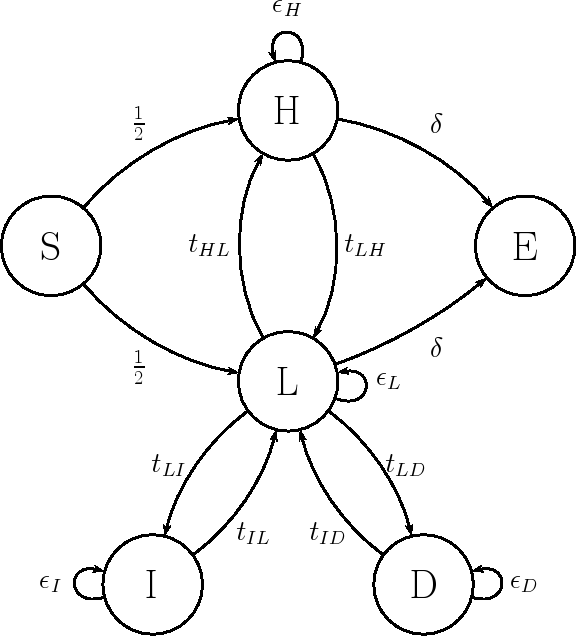
\includegraphics[width=0.5\textwidth]{figures/velvetrope/HMMpic.png}
        \caption[HMM for synthetic NW comparison]{The HMM for generating the test sequence. There are 6 states, Start(S), High Density(H) where there is a 0.63 chance of sampling from the sequence of interest and 0.37 chance of random, Low Density(L) where all sampling is random, Deletion(D) where we shorten the sequence, Insertion(I) where we add a random element to the sequence but don't increment the position we are comparing ourselves to in the sequence of interest, and End(E)}
	\label{fig:99}
\end{figure}

The parameter values are set as follows:

\begin{equation}
    \left\{\begin{tabular}{c} $\delta$ = $\frac{1}{800}$ \\ $t_{HL} = t_{LH} = \frac{1}{20}$ \\ $t_{LD} = t_{LI} = \frac{1}{20}$ \\ $\epsilon_{D} = \epsilon_{I} = \frac{3}{5}$ \\ $t_{IL} = t_{ID} = \frac{2}{5}$ \\ $\epsilon_{H} = \frac{19}{20} - \delta$ \\ $\epsilon_{L} = \frac{17}{20} - \delta$ \end{tabular} \right.
\end{equation}

We use the BLOSUM62 matrix \cite{Henikoff1992}, and a relatively high deletion penalty (equal to the highest transfer) and an emission rate of a quarter of that.

\begin{figure}[hpt]
	\centering
		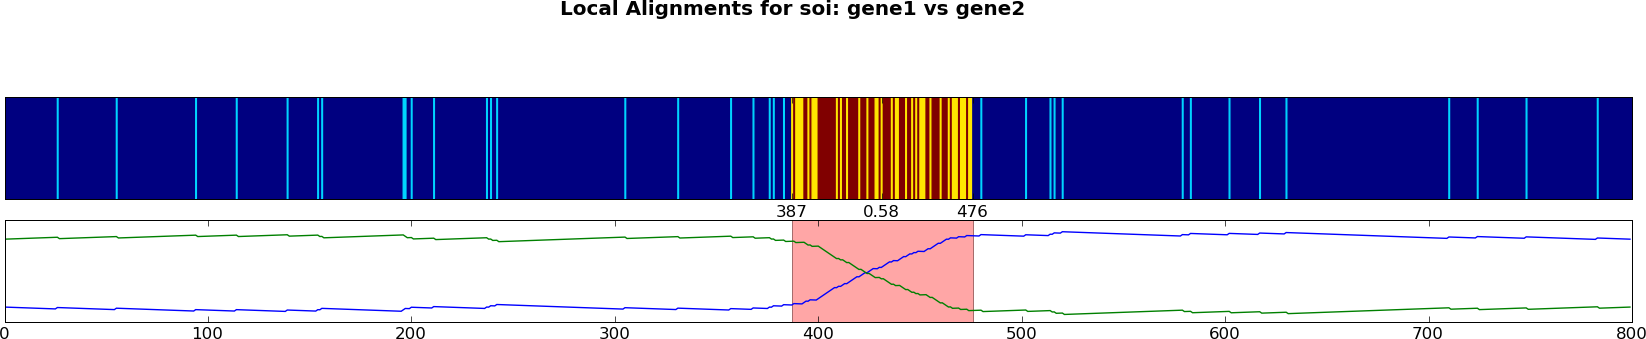
\includegraphics[width=1.0\textwidth]{figures/velvetrope/hmm1_1.png}
        \caption[Local Velvetrope filter of NW HMM test]{The local filter information on the single line of high density returned from the global filter}
	\label{fig:05}
\end{figure}

\begin{figure}[hpt]
	\centering
		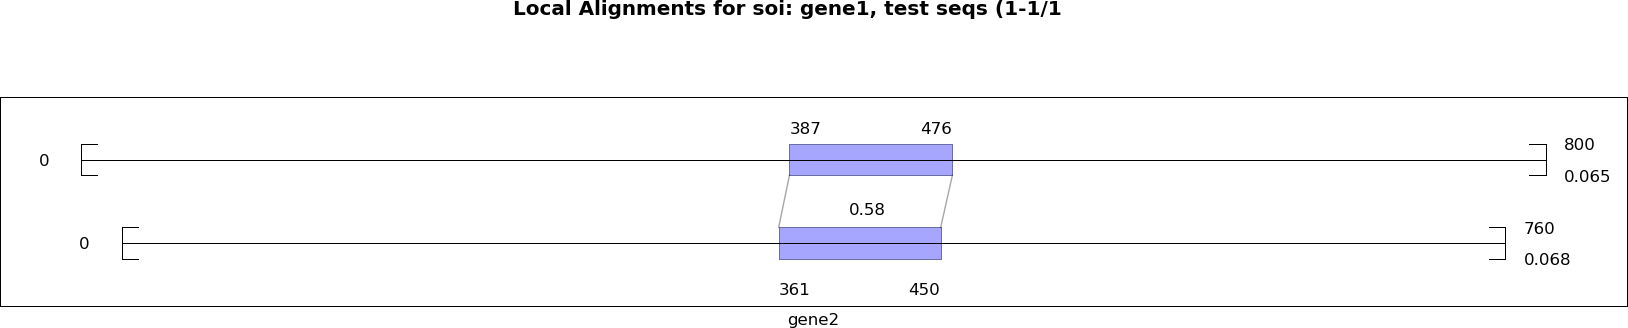
\includegraphics[width=1.0\textwidth]{figures/velvetrope/hmm1_2.png}
        \caption[Topological information of NW HMM test]{Topological information on the relative position and density of the alignment}
	\label{fig:06}
\end{figure}

Below is the area of local alignment as determined by Velvetrope as compared to the same region aligned by NW.

\begin{flushleft}
    \singlespacing
\footnotesize 
\texttt{RES: [388,469] of gene1}           

\texttt{R\textcolor{red}{V}RGYI\textcolor{red}{V}\textcolor{red}{W}I\textcolor{red}{K}TLD\textcolor{red}{P}\textcolor{red}{W}\textcolor{red}{H}\textcolor{red}{I}\textcolor{red}{N}\textcolor{red}{S}\textcolor{red}{K}\textcolor{red}{C}\textcolor{red}{F}G\textcolor{red}{G}S\textcolor{red}{D}\textcolor{red}{I}M\textcolor{red}{C}\textcolor{red}{T}\textcolor{red}{H}\textcolor{red}{D}\textcolor{red}{T}H\textcolor{red}{I}\textcolor{red}{V}\textcolor{red}{Y}H\textcolor{red}{H}\textcolor{red}{V}\textcolor{red}{Y}RK\textcolor{red}{S}E\textcolor{red}{L}\textcolor{red}{H}\textcolor{red}{E}\textcolor{red}{K}M\textcolor{red}{L}ES\textcolor{red}{N}\textcolor{red}{R}\textcolor{red}{F}C\textcolor{red}{A}\textcolor{red}{V}R\textcolor{red}{Q}I\textcolor{red}{H}HSH\textcolor{red}{A}\textcolor{red}{D}H\textcolor{red}{F}\textcolor{red}{W}\textcolor{red}{R}\textcolor{red}{L}V\textcolor{red}{N}\textcolor{red}{V}\textcolor{red}{E}A\textcolor{red}{V}FCW} \\
\texttt{C\textcolor{red}{V}EKEY\textcolor{red}{V}\textcolor{red}{W}F\textcolor{red}{K}YNA\textcolor{red}{P}\textcolor{red}{W}\textcolor{red}{H}\textcolor{red}{I}\textcolor{red}{N}\textcolor{red}{S}\textcolor{red}{K}\textcolor{red}{C}\textcolor{red}{F}R\textcolor{red}{G}G\textcolor{red}{D}\textcolor{red}{I}H\textcolor{red}{C}\textcolor{red}{T}\textcolor{red}{H}\textcolor{red}{D}\textcolor{red}{T}W\textcolor{red}{I}\textcolor{red}{V}\textcolor{red}{Y}L\textcolor{red}{H}\textcolor{red}{V}\textcolor{red}{Y}LT\textcolor{red}{S}N\textcolor{red}{L}\textcolor{red}{H}\textcolor{red}{E}\textcolor{red}{K}G\textcolor{red}{L}TG\textcolor{red}{N}\textcolor{red}{R}\textcolor{red}{F}T\textcolor{red}{A}\textcolor{red}{V}V\textcolor{red}{Q}H\textcolor{red}{H}IAM\textcolor{red}{A}\textcolor{red}{D}V\textcolor{red}{F}\textcolor{red}{W}\textcolor{red}{R}\textcolor{red}{L}T\textcolor{red}{N}\textcolor{red}{V}\textcolor{red}{E}W\textcolor{red}{V}KVG}

\texttt{RES: [362,443] of gene2}

\texttt{RES: [470,476] of gene1}

\texttt{\textcolor{red}{N}SFY\textcolor{red}{Q}TG} \\
\texttt{\textcolor{red}{N}YAF\textcolor{red}{Q}YA}

\texttt{RES: [444,450] of gene2}

\normalsize
\normalspacing
\end{flushleft}

We note that by trying to align the random sections earlier and later in the sequence the algorithm fails to accurately pick up this area of high local alignment.

\begin{flushleft}
    \singlespacing
\footnotesize 
\texttt{RES: [425,506]}

\texttt{\textcolor{red}{R}VRGYI-VWI--KTL\textcolor{red}{D}PWH\textcolor{red}{I}NS--\textcolor{red}{K}C\textcolor{red}{F}G\textcolor{red}{G}SDIM-\textcolor{red}{C}THDTHI\textcolor{red}{V}YHHV\textcolor{red}{Y}RKS-ELHE\textcolor{red}{K}MLESNRF-\textcolor{red}{C}AVRQ--\textcolor{red}{I}HHS\textcolor{red}{H}ADHFWR} \\
\texttt{\textcolor{red}{R}-NKKNRT-CKNERI\textcolor{red}{D}GTC\textcolor{red}{I}-FWL\textcolor{red}{K}-\textcolor{red}{F}A\textcolor{red}{G}TP-SC\textcolor{red}{C}V-EKEY\textcolor{red}{V}WFK-\textcolor{red}{Y}NAPWHINS\textcolor{red}{K}CFRGGDIH\textcolor{red}{C}-THDTW\textcolor{red}{I}VYL\textcolor{red}{H}V-YLTS}

\texttt{RES: [425,506]}

\texttt{RES: [507,525]}

\texttt{-\textcolor{red}{L}VNVEAVFCWNSF-Y\textcolor{red}{Q}TG} \\
\texttt{N\textcolor{red}{L}HEKGLTGNRFTAVV\textcolor{red}{Q}-H}

\texttt{RES: [507,525]}

\normalsize
\normalspacing
\end{flushleft}

\subsection{Comparison to NW: Pathological Transposition}

Now we look at a pathological example where we generate the sequence of interest randomly as before.

For the test sequence we generate the first 200 residues randomly. Then for the next 100 we draw from SOI[500:600] at a rate of .63 and random otherwise. This is followed by another 200 random residues. Then for the next 100 we draw from SOI[200:300] at a rate of .63 and random otherwise. This is followed by a final 200 random sequences.

This gives the effect of SOI = [random, gene1, random, gene2, random] and TS = [random, gene2, random, gene1, random].

NW and Velvetrope are both run on this example with the following results and local alignments

\begin{figure}[hpt]
	\centering
		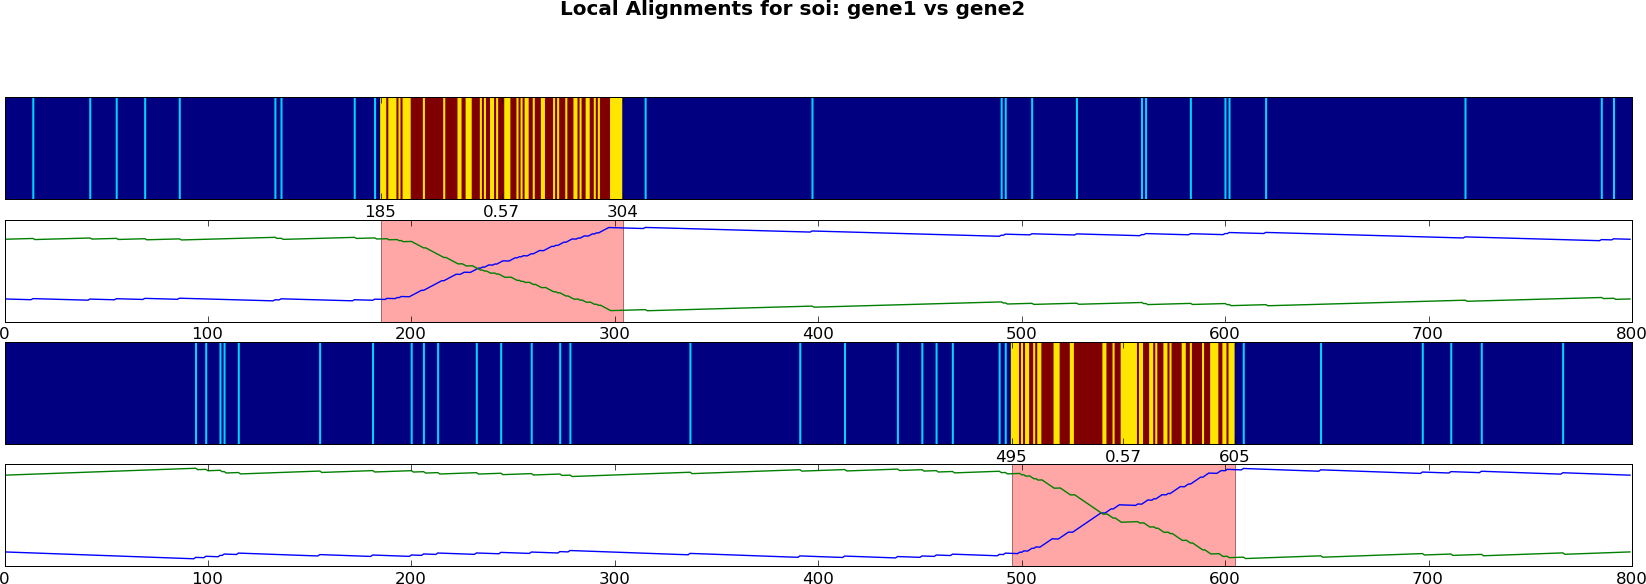
\includegraphics[width=1.0\textwidth]{figures/velvetrope/path1_1.png}
        \caption[Local Velvetrope filter for NW trasposition test]{The local filter information on the two lines of high density returned from the global filter}
	\label{fig:07}
\end{figure}

\begin{figure}[hpt]
	\centering
		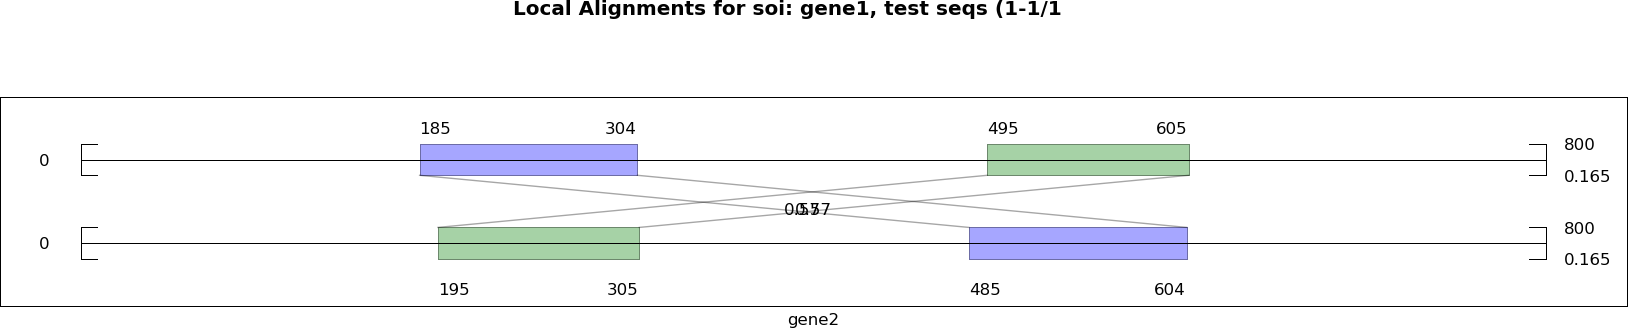
\includegraphics[width=1.0\textwidth]{figures/velvetrope/path1_2.png}
	\caption[Topological information of NW transposition test]{Topological information on the relative position and density of the alignments. We can see that they are transposed as expected. The densities are 0.57 and 0.55 respectively.}
	\label{fig:08}
\end{figure}

Below is the area of local alignment as determined by Velvetrope for the first conserved section.

\begin{flushleft}
    \singlespacing
\footnotesize
\texttt{RES: [186,267] of gene1}           

\texttt{GAN\textcolor{red}{H}KYQV\textcolor{red}{H}Q\textcolor{red}{P}LNAM\textcolor{red}{Y}\textcolor{red}{Y}\textcolor{red}{Q}\textcolor{red}{G}\textcolor{red}{S}\textcolor{red}{T}H\textcolor{red}{H}\textcolor{red}{F}\textcolor{red}{C}\textcolor{red}{E}\textcolor{red}{L}\textcolor{red}{K}\textcolor{red}{R}\textcolor{red}{T}\textcolor{red}{W}V\textcolor{red}{N}\textcolor{red}{Y}\textcolor{red}{T}\textcolor{red}{W}\textcolor{red}{I}\textcolor{red}{E}MC\textcolor{red}{I}\textcolor{red}{I}CNK\textcolor{red}{C}\textcolor{red}{N}\textcolor{red}{E}\textcolor{red}{C}G\textcolor{red}{V}V\textcolor{red}{V}\textcolor{red}{Y}NQ\textcolor{red}{S}R\textcolor{red}{L}\textcolor{red}{K}\textcolor{red}{V}WCS\textcolor{red}{I}\textcolor{red}{C}\textcolor{red}{H}S\textcolor{red}{P}A\textcolor{red}{E}VK\textcolor{red}{Q}\textcolor{red}{D}T\textcolor{red}{I}\textcolor{red}{M}\textcolor{red}{Y}LC\textcolor{red}{H}} \\         
\texttt{LNP\textcolor{red}{H}QPHA\textcolor{red}{H}Y\textcolor{red}{P}CDNN\textcolor{red}{Y}\textcolor{red}{Y}\textcolor{red}{Q}\textcolor{red}{G}\textcolor{red}{S}\textcolor{red}{T}I\textcolor{red}{H}\textcolor{red}{F}\textcolor{red}{C}\textcolor{red}{E}\textcolor{red}{L}\textcolor{red}{K}\textcolor{red}{R}\textcolor{red}{T}\textcolor{red}{W}Q\textcolor{red}{N}\textcolor{red}{Y}\textcolor{red}{T}\textcolor{red}{W}\textcolor{red}{I}\textcolor{red}{E}LR\textcolor{red}{I}\textcolor{red}{I}LIF\textcolor{red}{C}\textcolor{red}{N}\textcolor{red}{E}\textcolor{red}{C}S\textcolor{red}{V}S\textcolor{red}{V}\textcolor{red}{Y}LT\textcolor{red}{S}A\textcolor{red}{L}\textcolor{red}{K}\textcolor{red}{V}IGI\textcolor{red}{I}\textcolor{red}{C}\textcolor{red}{H}P\textcolor{red}{P}Y\textcolor{red}{E}LE\textcolor{red}{Q}\textcolor{red}{D}K\textcolor{red}{I}\textcolor{red}{M}\textcolor{red}{Y}NT\textcolor{red}{H}}

\texttt{RES: [486,567] of gene2}

\texttt{RES: [268,304] of gene1}

\texttt{\textcolor{red}{K}\textcolor{red}{F}\textcolor{red}{C}E\textcolor{red}{T}V\textcolor{red}{E}\textcolor{red}{M}\textcolor{red}{H}Q\textcolor{red}{E}\textcolor{red}{M}\textcolor{red}{D}QI\textcolor{red}{A}C\textcolor{red}{H}\textcolor{red}{A}YE\textcolor{red}{G}\textcolor{red}{I}W\textcolor{red}{L}S\textcolor{red}{H}\textcolor{red}{V}\textcolor{red}{K}\textcolor{red}{D}\textcolor{red}{V}FKCEVN} \\
\texttt{\textcolor{red}{K}\textcolor{red}{F}\textcolor{red}{C}T\textcolor{red}{T}W\textcolor{red}{E}\textcolor{red}{M}\textcolor{red}{H}S\textcolor{red}{E}\textcolor{red}{M}\textcolor{red}{D}DS\textcolor{red}{A}E\textcolor{red}{H}\textcolor{red}{A}HW\textcolor{red}{G}\textcolor{red}{I}F\textcolor{red}{L}P\textcolor{red}{H}\textcolor{red}{V}\textcolor{red}{K}\textcolor{red}{D}\textcolor{red}{V}NALFLK}

\texttt{RES: [568,604] of gene2}

\normalsize
\normalspacing
\end{flushleft}

Below is the area of local alignment as determined by Velvetrope for the second conserved section as compared to the same region aligned by NW.

\begin{flushleft}
\singlespacing
\footnotesize 
\texttt{RES: [496,577] of gene1}           

\texttt{VNEK\textcolor{red}{P}Y\textcolor{red}{C}GE\textcolor{red}{T}\textcolor{red}{M}H\textcolor{red}{K}AF\textcolor{red}{S}\textcolor{red}{M}\textcolor{red}{V}\textcolor{red}{S}\textcolor{red}{C}\textcolor{red}{R}WCI\textcolor{red}{E}\textcolor{red}{V}\textcolor{red}{L}\textcolor{red}{W}\textcolor{red}{G}VC\textcolor{red}{G}\textcolor{red}{R}\textcolor{red}{S}\textcolor{red}{L}\textcolor{red}{H}\textcolor{red}{Q}\textcolor{red}{A}\textcolor{red}{E}\textcolor{red}{K}\textcolor{red}{N}\textcolor{red}{R}\textcolor{red}{E}\textcolor{red}{V}\textcolor{red}{P}AA\textcolor{red}{V}\textcolor{red}{H}\textcolor{red}{N}T\textcolor{red}{V}\textcolor{red}{K}\textcolor{red}{C}FEMMYPRQ\textcolor{red}{M}HD\textcolor{red}{V}\textcolor{red}{A}\textcolor{red}{T}PE\textcolor{red}{H}K\textcolor{red}{M}\textcolor{red}{H}\textcolor{red}{Y}SV\textcolor{red}{V}K\textcolor{red}{C}\textcolor{red}{R}\textcolor{red}{G}} \\
\texttt{IYWW\textcolor{red}{P}R\textcolor{red}{C}ID\textcolor{red}{T}\textcolor{red}{M}D\textcolor{red}{K}RT\textcolor{red}{S}\textcolor{red}{M}\textcolor{red}{V}\textcolor{red}{S}\textcolor{red}{C}\textcolor{red}{R}IGR\textcolor{red}{E}\textcolor{red}{V}\textcolor{red}{L}\textcolor{red}{W}\textcolor{red}{G}ML\textcolor{red}{G}\textcolor{red}{R}\textcolor{red}{S}\textcolor{red}{L}\textcolor{red}{H}\textcolor{red}{Q}\textcolor{red}{A}\textcolor{red}{E}\textcolor{red}{K}\textcolor{red}{N}\textcolor{red}{R}\textcolor{red}{E}\textcolor{red}{V}\textcolor{red}{P}QV\textcolor{red}{V}\textcolor{red}{H}\textcolor{red}{N}M\textcolor{red}{V}\textcolor{red}{K}\textcolor{red}{C}LKCVGVSK\textcolor{red}{M}DM\textcolor{red}{V}\textcolor{red}{A}\textcolor{red}{T}FH\textcolor{red}{H}A\textcolor{red}{M}\textcolor{red}{H}\textcolor{red}{Y}EP\textcolor{red}{V}M\textcolor{red}{C}\textcolor{red}{R}\textcolor{red}{G}}

\texttt{RES: [196,277] of gene2}

\texttt{RES: [578,605] of gene1}

\texttt{\textcolor{red}{P}\textcolor{red}{C}GL\textcolor{red}{C}\textcolor{red}{N}F\textcolor{red}{I}\textcolor{red}{C}\textcolor{red}{D}\textcolor{red}{T}\textcolor{red}{D}P\textcolor{red}{L}\textcolor{red}{M}\textcolor{red}{K}GFDE\textcolor{red}{P}\textcolor{red}{N}KN\textcolor{red}{W}MTI} \\
\texttt{\textcolor{red}{P}\textcolor{red}{C}VE\textcolor{red}{C}\textcolor{red}{N}A\textcolor{red}{I}\textcolor{red}{C}\textcolor{red}{D}\textcolor{red}{T}\textcolor{red}{D}Q\textcolor{red}{L}\textcolor{red}{M}\textcolor{red}{K}INIR\textcolor{red}{P}\textcolor{red}{N}SD\textcolor{red}{W}TVV}

\texttt{RES: [278,305] of gene2}

\normalsize
\normalspacing
\end{flushleft}

This algorithm is clearly not set up to deal with transposed conserved regions and it fails as expected.

\begin{flushleft}
\singlespacing
\footnotesize
 
\texttt{RES: [556,637]}

\texttt{VNEK\textcolor{red}{P}Y\textcolor{red}{C}GETMHKAFSMV-SCRW\textcolor{red}{C}I\textcolor{red}{E}V\textcolor{red}{L}WGVCGRSLHQA-\textcolor{red}{E}KN\textcolor{red}{R}EVPAAVHNTVK\textcolor{red}{C}FEMM\textcolor{red}{Y}-P--RQM-HDVAT\textcolor{red}{P}EHKMHYS} \\
\texttt{AH-Y\textcolor{red}{P}-\textcolor{red}{C}-DN-N-YY-QGSTIHF\textcolor{red}{C}-\textcolor{red}{E}-\textcolor{red}{L}KRT-WQN-YTWI\textcolor{red}{E}L-\textcolor{red}{R}-I-ILIF-CNE\textcolor{red}{C}SVSV\textcolor{red}{Y}LTSALKVIGIICH\textcolor{red}{P}PYELEQD}

\texttt{RES: [556,637]}

\texttt{RES: [638,674]}

\texttt{VVKCRGPCG-L\textcolor{red}{C}NFICDTDPL\textcolor{red}{M}K-GFD\textcolor{red}{E}PNKN\textcolor{red}{W}-MTI} \\
\texttt{KI-MYN-THKF\textcolor{red}{C}T-TWEMHSE\textcolor{red}{M}DDS-A\textcolor{red}{E}-HAH\textcolor{red}{W}GIFL}

\texttt{RES: [638,674]}

\normalsize
\normalspacing
\end{flushleft}

\section{Multiple Sequence Alignment}

Multi-domain proteins have traditionally been cumbersome to Multiple Sequence Alignment (MSA) algorithms like MUSCLE \cite{MUSCLE} and DIALIGN-TX \cite{DIALIGN-TX} like the 31 multi-domain lectin proteins in Reference 8 of BAliBASE v3 \cite{Balibase}. The two domains for lectin are transposed for 4 of the organisms and are ordered ``correctly'' for the other 27 in the reference database (See figure \ref{fig:vr04}). Because Velvetrope works independent of order it allows us to find transposed domains from within a protein such as this with relative ease and compute a probable, non-traditional MSA.

Comparing a sequence of interest against a large set of test sequences allows Velvetrope to find the areas within the sequence of interest that are homologous to multiple test sequences. By combining this information across many sequences (as in figure \ref{fig:vr05}) we make a histogram of which residues were matches and in the club across many test sequences. We are able to discern areas of possible multiple alignment from within the sequence of interest in this fashion. By looking at the areas within the sequence of interest which are consistently identical to test sequences or in the club we can generate regular expressions of sequence that can be readily re-mapped onto the sequence of interest, representing a non-traditional multiple alignment.  This allows us to find a probable MSA and because Velvetrope only compares a single sequence of interest against a larger set we can use this to quickly append a new sequence to a multiple alignment multiple orders of magnitude faster than traditional methods which would have to recalculate the entire MSA for every appended sequence.

Traditional methods, like those in BAliBASE, have to be prompted with domain information to make sense of a multi-domain protein at all. Even with this information they only align the prompted domain and merely append the other domain(s) around the domain of interest. This results in a MSA that does not represent the true alignment between the proteins. Velvetrope is able to produce a shorter MSA with all domains represented without any prior information. In Figure \ref{fig:vr06} we look at two MSAs in which BAliBASE was prompted with the two lectin domains and it generates an non-intuitive alignment. While using just a single sequence of interest we are able to find both domains and re-map them onto that sequence and generate a much more compact and representative probable MSA very quickly.

 \begin{figure}[htp]%figure5
 \centerline{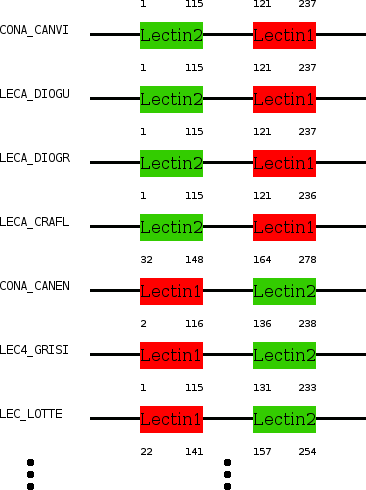
\includegraphics[width=0.5\textwidth]{figures/velvetrope/BAliBASEsnap2v2.png}}
 \caption[Multiple alignment reference]{The lectin sequences from \textit{Reference 8 - Circular Permutations} of BAliBASE3. The reference contains 31 two-domain lectin proteins from a myriad of organisms. In 4 of the sequences the Lectin2 domain comes before the Lectin1 domain, the opposite for the remaining 27. This presents a problem for most multiple alignment algorithms which will try to align one domain or the other.}
 	\label{fig:vr04}
 \end{figure}
 
 \begin{figure}[htp]%figure6
 \centerline{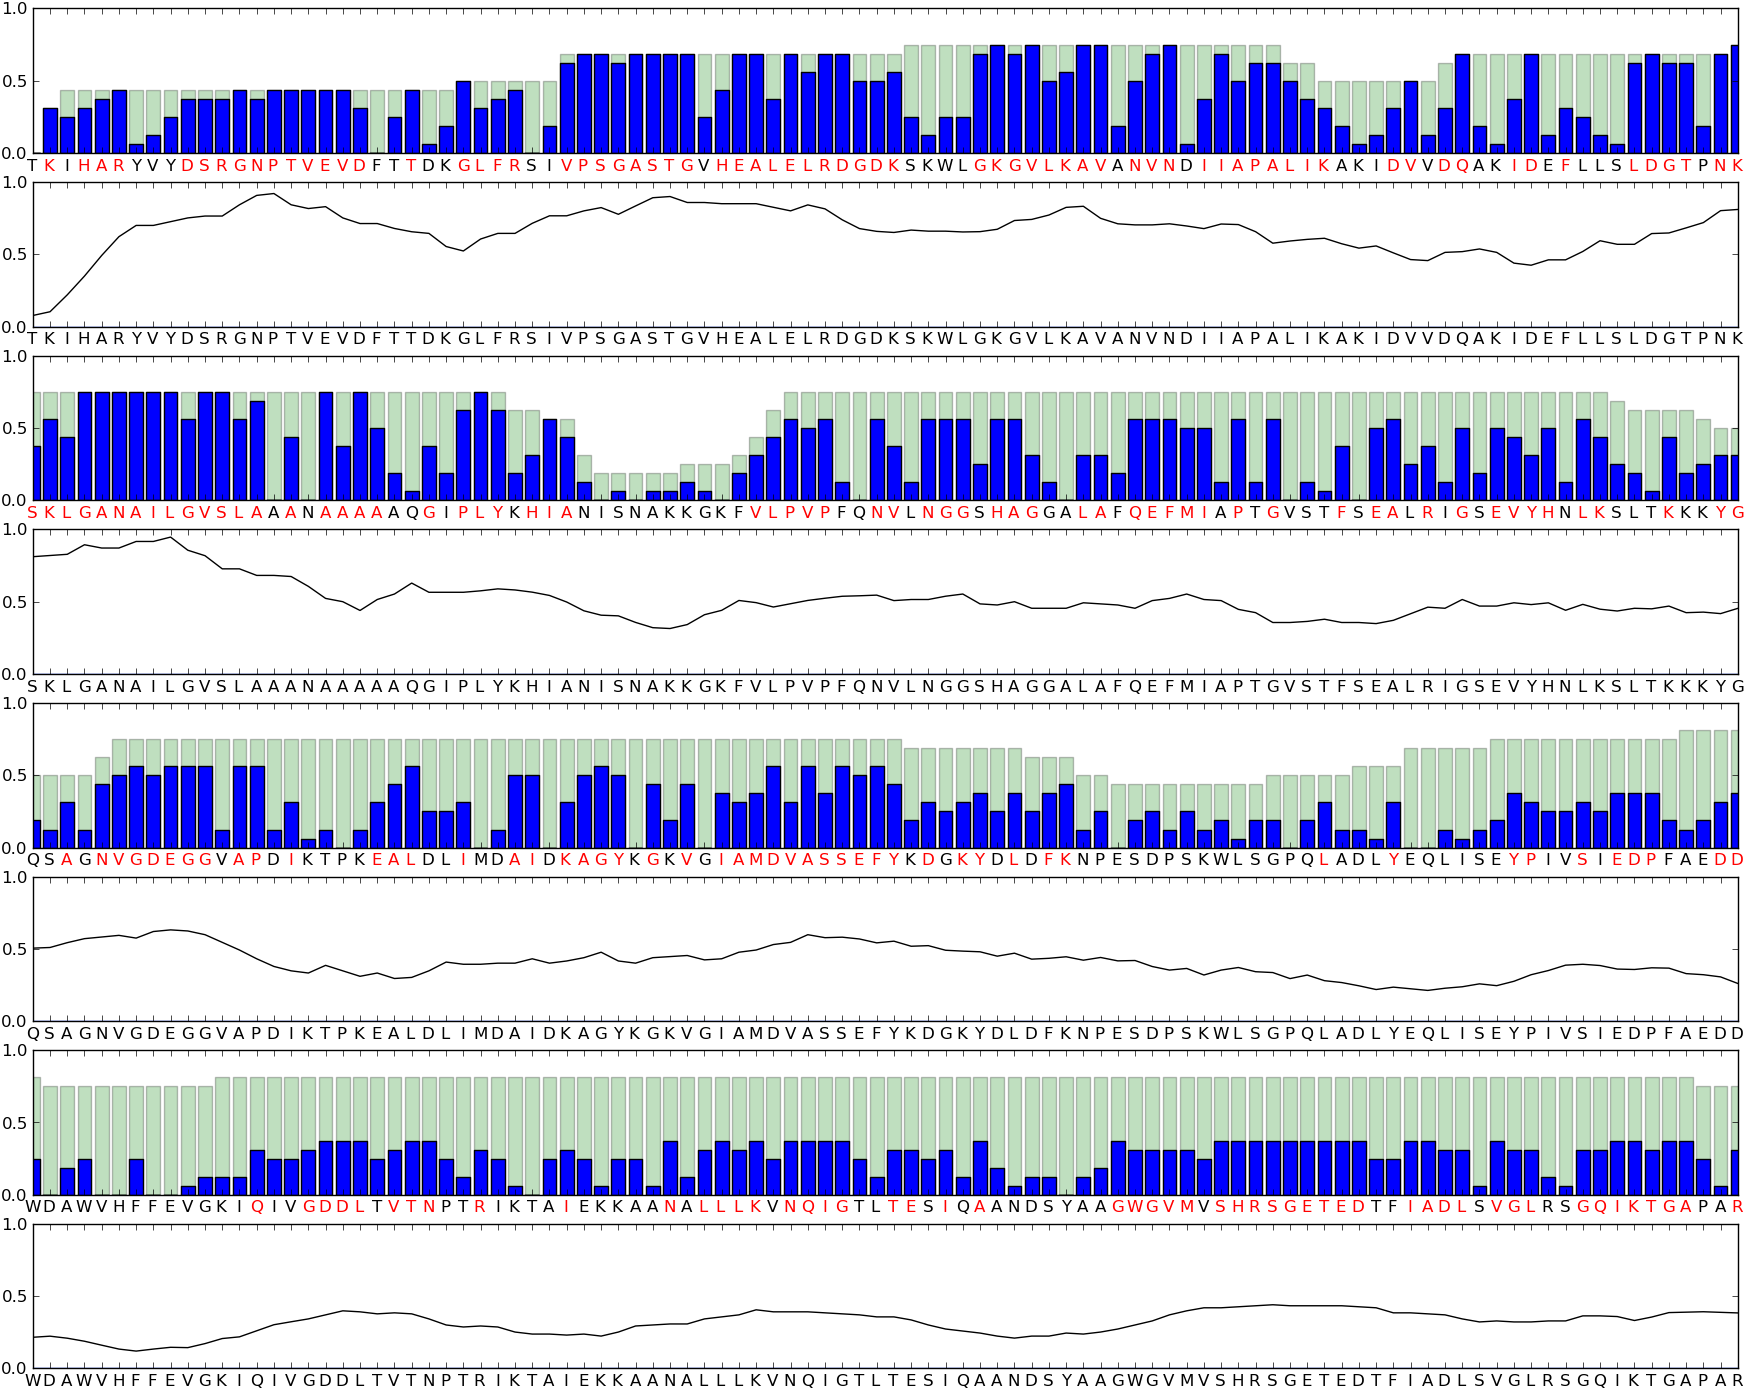
\includegraphics[width=\textwidth]{figures/velvetrope/COMBO1.png}}
 \caption[Velvetrope per-base output]{We see that by combining the information about shared identity (solid, blue columns) and club membership
(light, always larger, green columns) from a single sequence of interest across many test sequences we can
find the areas of the sequence of interest that are shared among a large percentage of the whole set. This
information, shown for the lectin protien from BAliBASE reference 8, can be used to determine where the
two protien domains are (areas where the columns are high) and create a probable MSA.}
 	\label{fig:vr05}
 \end{figure}
 
 \begin{figure*}[htp]%figure6
 \centerline{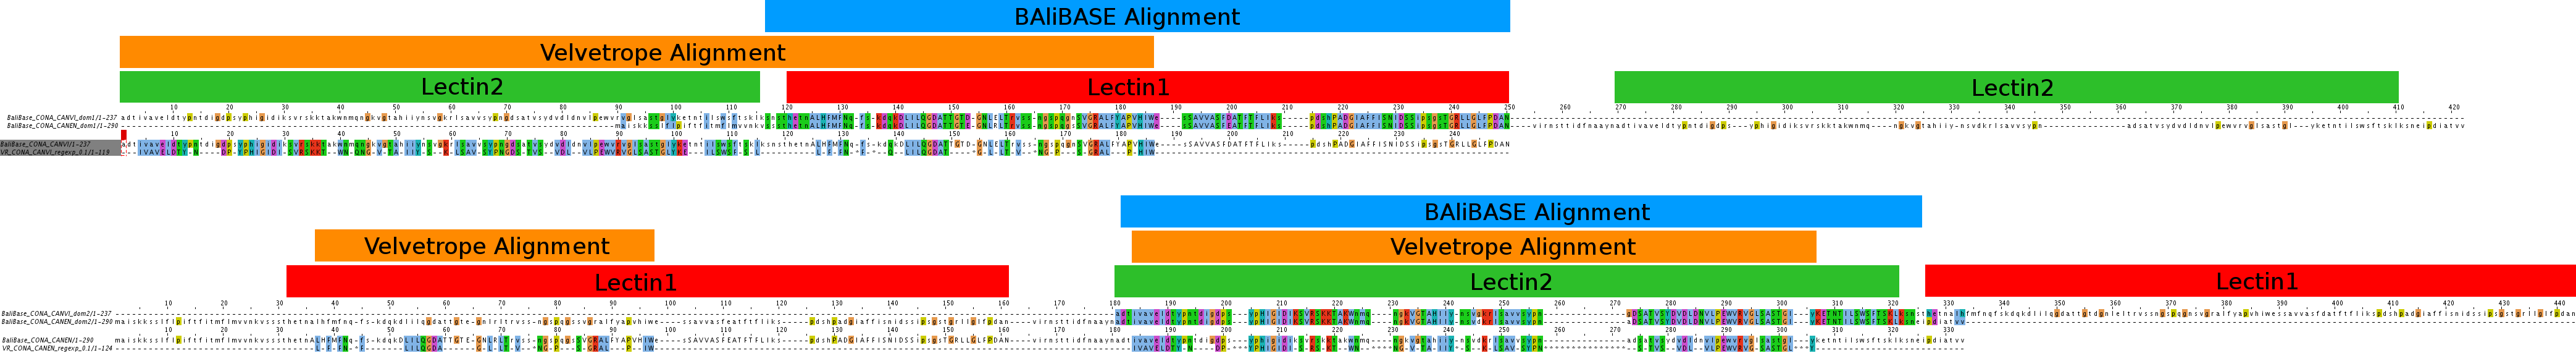
\includegraphics[width=\textwidth]{figures/velvetrope/Alignments.png}}
 \caption[Multiple sequence alignments]{Two sets of alignments of the two-domain lectin protein reference. Red corresponds to the Lectin1 domain. Green is the Lectin2 domain. Orange is the Velvetrope alignment. Blue is the BAliBASE alignment. BAliBASE resolves the two-domain problem by manually specifying which domain to align (Lectin1 in the first alignment, Lectin2 in the second). This causes the aligner to append whatever domain not specified to the beginning or end of the alignment. Velvetrope is order independent which allows it to pick out areas of homology regardless of position in the sequence without any expert tuning. Lectin1 suffers from low homologous identity in the latter part of its domain and is therefore not picked up by Velvetrope, but is aligned by the non-homology components of BAliBASE.}
 	\label{fig:vr05}
 \end{figure*}


\section*{Local alignment comparison}

While Velvetrope does not perform a local alignment in the traditional sense it is able to find areas of high local homology between sequences, regardless of order or k-mer density, that are highly probable areas of local alignment. Velvetrope compares well at a visual level to standard algorithms like BLAST \cite{BLAST} and HMMer \cite{Eddy98} and the C/CUDA implementation executes at the same order of magnitude or faster than these methods. Velvetrope is very susceptible to high indel rates within a conserved region (shifts the offsets) but has been shown to equal or outperform these other methods in areas of low indel rate especially when there are only short $k$-mers within the homologous region between the two sequences.

\section{Comparison to other methods} % (fold)
\label{sec:Comparison to other methods}

To compare the sensitivity and specificity of Velvetrope to other popular methods such as BLAST \cite{BLAST} and HMMer \cite{Eddy98} we contrast the regions of similarity that each algorithm reports when comparing genes from {\it E. Coli} and {\it Bacillus subtilis} \cite{GenBank}. Using each programs default parameters we obtain the results:

\begin{table}[h]
    \begin{center}
\begin{tabular}{c|c|c}
    Method & Reported Bases Similar & Reported Regions Similar \\
    \hline
    BLAST & 1112 & 3 \\
    HMMer & 1081 & 5 \\
    Velvetrope & 842 & 7
\end{tabular}
\label{vr_comp_table}
\end{center}
\end{table}
We note that the default settings of Velvetrope are much more specific and less sensitive than both BLAST and HMMer. By modifying the parameters of the two filters we can increase the sensitivity at the cost of the specificity. Using the default parameters allows us to use Velvetrope as a quick first-pass algorithm to find areas of high identity that could then be expanded by algorithms such as BLAST and HMMer that are significantly more computationally intensive.

\begin{figure}[htp]%figure3
 \centerline{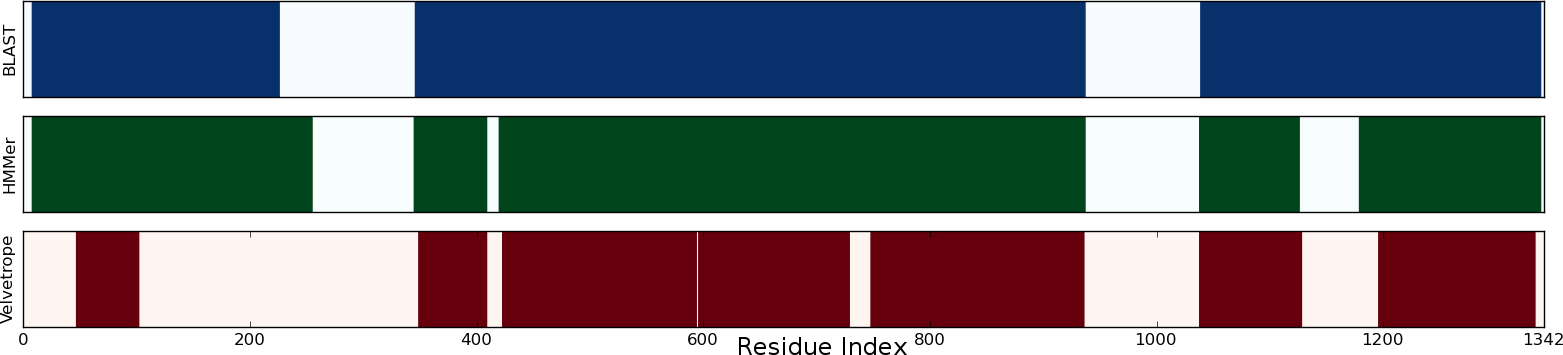
\includegraphics[width=\textwidth]{figures/velvetrope/compare6.png}}
 \caption[Velvetrope vs. HMMer and BLAST]{The regions within {\it E. Coli} that each algorithm found identity in when compared to {\it Bacillus subtilis}.}
 	\label{VRcompare1}
 \end{figure}

 \begin{figure}[htp]%figure3
 \centerline{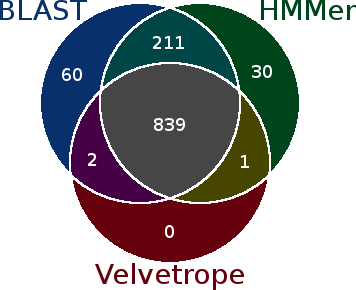
\includegraphics[width=0.5\textwidth]{figures/velvetrope/compare5.png}}
 \caption[Comparison Venn diagram]{The bases within {\it E. Coli} that each algorithm found identity in when compared to {\it Bacillus subtilis} and their respective overlaps between the algorithms.}
 	\label{VRcompare2}
 \end{figure}

% section Comparison to other methods (end)

% chapter Velvetrope Results (end)

\chapter{Velvetrope Implementation} % (fold)
\label{cha:Velvetrope Implementation}

Velvetrope is designed to be easily parrallelizeable and far less complex than other methods. In figure \ref{fig:vr06} we compare the implementation of Vevletrope to that of BLAST \cite{BLAST}. We do not show HMMer on the plot because it is so computationally expensive that it does not fit, requiring many minutes for comparing only a few hundred sequences.

\begin{figure}[htp]%figure3
 \centerline{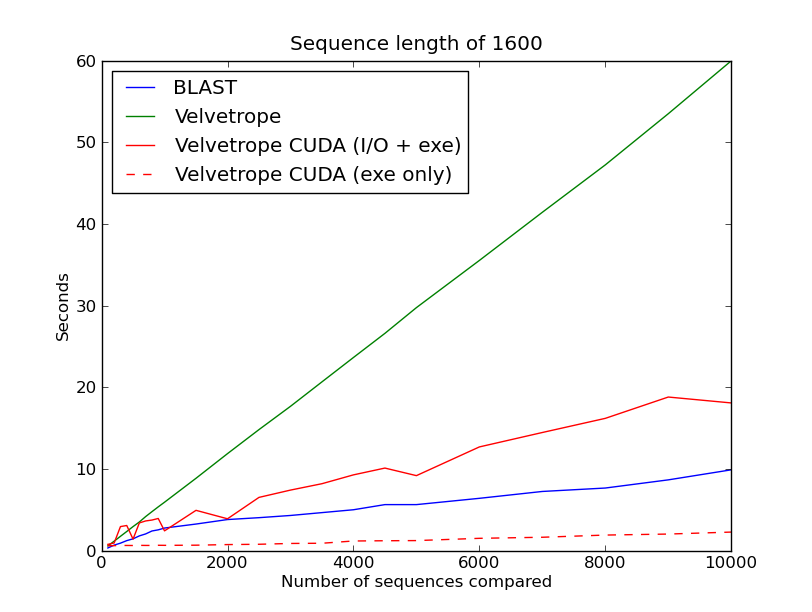
\includegraphics[width=\textwidth]{figures/velvetrope/timersSC.png}}
 \caption[Velvetrope timings]{The sequential C implementation of Velvetrope can compare 10,000 sequences to a SOI in almost exactly a minute. BLAST, which has been optimized for many years across many platforms can perform the same number of calculations in 20 seconds. The CUDA implementation of Velvetrope can execute the algorithm in under 3 seconds, but requires another 15 seconds to load the data onto the GPGPU across the PCI-E bus. If the sequence information is cached on the GPGPU then this memory transfer step is alleviated and Velvetrope can compare SOIs against these cached sequences at a rate much faster than BLAST.}
 	\label{fig:vr06}
 \end{figure}

Velvetrope is able to find areas of sequence homology quickly and efficiently across multiple sequences. It finds these areas of high shared identity density in a way that allows it to locate areas otherwise missed by $k$-mer based or position dependent methods. It is able to correctly find probable alignments in multi-domain proteins and pairwise local areas of similarity between distant homologies. Its low order of computational complexity, $\mathcal O$($N$) where $N$ is the total length of the sequences
being compared, allows for it to scale with the data intensive challenges that fields like metagenomics and cancer genomics present.

We also present a freely available, open source implementation (both serial and parallel; in Python, C and CUDA) with easy to navigate HTML output similar to MEME \cite{MEME}. The API and documentation make it easily extendible and able to adapt to the future computationally intensive problems it is designed to address.

\section{Availability and requirements}
 \begin{itemize}
  \item \textbf{Project name:} Velvetrope
  \item \textbf{Project home page:} velvetrope.sourceforge.net
  \item \textbf{Operating systems:} Linux 32/64-bit, Mac OSX, Windows (Cygwin)
  \item \textbf{Programming languages:} Python, C, CUDA, HTML/CSS
  \item \textbf{Other requirements:} Some python packages, see documentation
  \item \textbf{License:} GPL v2.01
 \end{itemize}

% chapter Velvetrope Implementation (end)

% part Velvetrope (end)

\appendix
\chapter{Appendix}

\section{Computational Resources}

\subsection{Code Repository}

All code written for this thesis and each project is open source and can be found on github at (www.github.com/sc932).

See individual projects for licences, all open source.

\subsection{Workstation}

All speed tests using wall clock time were performed on my personal workstation (originally built in 2008) with the following specifications (Table \ref{worktab})

\begin{table}[htp]
    \caption{Workstation configuration}
    \label{worktab}
    \begin{center}
\begin{tabular}{r|l}
    Operating Sytstem & Ubuntu 11.04 \\
    CPU & 2x Xeon 2.5Ghz Quad Core (8 cores) \\
    Memory & 32GB DDR400 \\
    GPU & NVIDIA GeForce 480 GTX (480 cores) \\
    HDD & 64GB SSD (150Mb/s read/write), 1TB Raid 10 (storage) \\
    Software & Python 2.7.1+, gcc 4.5.2, CUDA 4.1
\end{tabular}
\end{center}
\end{table}

\subsection{Hopper}

Some computations were performed on Hopper, a 153,216 processor (1.28PFlop) U.S. Department of Energy supercomputer at the National Energy Research Scientific Computing Center (NERSC), with the following specifications (Table \ref{hoppertab})

\begin{table}[htp]
    \caption{Hopper node configuration}
    \label{hoppertab}
    \begin{center}
\begin{tabular}{r|l}
    Operating Sytstem & Cray Linux Environment \\
    CPU & 2x AMD 12-core MagnyCours 2.1Ghz (24 cores) \\
    Memory & 32GB DDR1333 \\
    GPU & N/A \\
    HDD & via Interlink \\
    Software & Python 2.6, gcc 4.6.2
\end{tabular}
\end{center}
\end{table}


%\bibliography{ScottClark_thesis}

\begin{thebibliography}{}

%%%%%%%%%%%%%%%%%%%
        % ALE

\bibitem[Aird {\it et~al}., 2011]{Aird2011} Aird,D., Chen,W.S., Ross,M., Connolly,K., Meldrim,J., Russ,C., Fisher,S., Jaffe,D., Nusbaum,C., Gnirke,A. (2011) Analyzing and minimizing bias in Illumina sequencing libraries, {\it Genome Biology}, {\bf 12}, R18.
\bibitem[Altschul \textit{et~al}., 1990]{BLAST}
    Altschul, S.F., Gish W., Miller W., Myers E.W., Lipman D.J. (1990) Basic local alignment search tool. \textit{Journal of Molecular Biology}, \textbf{215}(3):403-410.
\bibitem[Altschul \textit{et~al}., 1997]{PSIBLAST}
Altshul, S.F., \textit{et~al}. (1997) Gapped BLAST and PSI-BLAST: a new generation pf protein database search programs. \textit{Nucleic Acids Research} \textbf{25}(17), 3389-3402.
\bibitem[Bailey \textit{et~al}., 2006]{MEME}
Bailey, T.L., \textit{et~al}. (2006) MEME: discovering and analyzing DNA and protein sequence motifs. \textit{Nucleic Acids Research} \textbf{34} W369-W373.
\bibitem[Brochu {\it et~al}., 2010]{Brochu2010} Brochu,E., Cora,V.M., de Freitas,N. (2010) A Tutorial on Bayesian Optimization of Expensive Cost Functions, with Application to Active User Modeling and Hierarchical Reinforcement Learning, {\it Computing Research Repository}, arXiv:1012.2599v1.
\bibitem[Choi {\it et~al}., 2008]{Choi2008} Choi,J.H., Kim,S., Tang,H., Andrews,J., Gilbert,D.G., Colbourne,J.K. (2008) A Machine Learning Approach to Combined Evidence Validation of Genome Assemblies, {\it BMC Bioinformatics}, {\bf 24}(6), 744-750.
\bibitem[Choudhary {\it et~al}., 2006]{Choudhary2006} Choudhary,M., Zanhua,X., Fu,Y.X., Kaplan,S. (2006) Genome analyses of three strains of Rhodobacter sphaeroides: evidence of rapid evolution of chromosome II, {\it Journal of Bacteriology}, {\bf 189}(5), 1914-1921.
\bibitem[Compo {\it et~al}., 2011]{Compo2011} Compo,G.P., Whitaker,J.S., Sardeshmukh,P.D., Matsui,N., Allan,R.J., {\it et~al}. (2011) The Twentieth Century Reanalysis Project, {\it Quarterly Journal of the Royal Meteorological Society}, {\bf 137}(654), 1-28.
\bibitem[Costello {\it et~al}., 2009]{Costello2009} Costello,E.K., Lauber,C.L., Hamady,M., Fierer,N., Gordon,J.I., Knight,R. (2009) Bacterial community variation in human body habitats across space and time, {\it Science}, {\bf 326}(5960), 1694-1697.
\bibitem[Durbin {\it et~al}., 2006]{Durbin06} 
    Durbin,R., Eddy,S., Krogh,A., Mitchison,G. (2006) Biological sequence analysis, $11^{th}$ edition.
\bibitem[Durfee {\it et~al}., 2008]{Durfee2008} Durfee,T., Nelson,R., Baldwin,S., Plunkett,G., Burland,V., Mau,B., Petrosino,J.F., Qin,X., Muzny,D.M., Ayele,M., {\it et~al}. (2008) The complete genome sequence of Escherichia coli DH10B: insights into the biology of a laboratory workhorse, {\it Journal of Bacteriology}, {\bf 190}(7), 2597-2606.
\bibitem[Eddy, 1998]{Eddy98} Eddy, S.R. (1998) Profile hidden Markov models. \textit{Bioinformatics}, \textbf{14}(9):755-763.
\bibitem[Edgar, 2004]{MUSCLE}
Edgar, R.C. (2004) MUSCLE: multiple sequence alignment with high accuracy and high throughput. \textit{Nucleic Acids Research} \textbf{32}(5) 1792-1797.
\bibitem[Edgar, 2010]{Edgar2010}
Edgar, R.C. (2010) Quality measures for protein alignment benchmarks. \textit{Nucleic Acids Research} \textbf{38}(7), 2145-2153.
\bibitem[Eid {\it et~al}., 2009]{Eid2009} Eid,J., Fehr,A., Gray,J., Luong,K., Lyle,J., Otto,G., Peluso,P., Rank,D., Baybayan,P., Bettman,B., {\it et~al}. (2009) Real-Time DNA Sequencing from Single Polymerase Molecules, {\it Science}, {\bf 323}(5910), 133-138.
\bibitem[Fu, 1994]{Fu1994} Fu,M.C. (1994) Optimization via Simulation: A Review, {\it Annals of Operations Research}, {\bf 53}(1), 199-247.
\bibitem[Fujimoto {\it et~al}., 2010]{Fujimoto2010} Fujimoto,A., Nakagawa,H., Hosono,N., Nakano,K., Abe,T., Boroevich,K.A., Nagasaki,M., Yamaguchi,R., Shibuya,T., Kubo,M., {\it et~al}. (2010) Whole-genome sequencing and comprehensive variant analysis of a Japanese individual using massively parallel sequencing, {\it Nature Genetics}, {\bf 42}, 931-936.
\bibitem[Gelman {\it et~al}., 2004]{Gelman2004} Gelman,A.B., Carlin,J.B., Stern,H.S., Rubin,D.B. (2004) Appendix A: Standard Probability Distributions, {\it Bayesian Data Analysis}, 2$^{\text{nd}}$ ed.
\bibitem[GenBank, 2009]{GenBank}
GenBank. (2009) \textit{Nucleic acids research}, doi:10.1093/nar/gkp1024.
\bibitem[Ginsbourger {\it et~al}., 2008]{Ginsbourger2008} Ginsbourger,D., Le Riche,R., Carraro,L. (2008) A Multi-points Criterion for Deterministic Parallel Global Optimization based on Gaussian Processes, {\it Unpublished results}.
\bibitem[Gnerre {\it et~al}., 2010]{Gnerre2010} Gnerre,S., MacCallum,I., Przybylski,D., Ribeiro,F., Burton,J., Walker,B., Sharpe,T., Hall,G., Shea,T., Sykes,S., {\it et~al}. (2010) High-quality draft assemblies of mammalian genomes from massively parallel sequence data, {\it Proceedings of the National Academy of Sciences USA}.
\bibitem[Haiminen {\it et~al}., 2011]{Haiminen2011} Haiminen,N., Kuhn,D.N., Parida,L., Rigoutsos,I. (2011) Evaluation of Methods for De Novo Genome Assembly from High-Throughput Sequencing Reads Reveals Dependencies That Affect the Quality of the Results, {\it PLoS ONE}, {\bf 6}(9).
\bibitem[Henikoff and Henikoff, 1992]{Henikoff1992}
    Henikoff,S. and Henikoff,J.G. (1992) Amino acid substitution matrices from protein blocks, {\it Proceedings of the National Academy of Sciences of the United States of America}, {\bf 89}(22), 10915-10919.
\bibitem[Hess {\it et~al}., 2011]{Hess2011} Hess,M., Sczyrba,A., Egan,R., Kim,T.W., Chokhawala,H., Schroth,G., Luo,S., Clark,D.S., Chen,F., Zhang,T., {\it et~al}. (2011) Metagenomic Discovery of Biomass-Degrading Genes and Genomes from Cow Rumen, {\it Science}, {\bf 331}(6016), 463-467.
\bibitem[Iverson {\it et~al}., 2012]{Iverson2012} Iverson,V., Morris,R.M., Frazar,C.D., Berthiaume,C.T., Morales,R.L., Armbrust,E.V. (2012) Untangling Genomes from Metagenomes: Revealing an Uncultured Class of Marine Euryarchaeota, {\it Science}, {\bf 335}(6068), 587-590.
\bibitem[Jones {\it et~al}., 1998]{Jones1998} Jones,D.R., Schonlau,M., Welch,W.J. (1998) Efficient Global Optimization of Expensive Black-Box Functions, {\it Journal of Global Optimization}, {\bf 13}, 455-492.
\bibitem[Kent {\it et~al}., 2002]{Kent2002} Kent,J.W., Sugnet,C.W., Furey,T.S., Roskin,K.M., Pringle,T.H., {\it et~al}. (2002) The Human Genome Browser at UCSC, {\it Genome Research}, {\bf 12}, 996-1006.
\bibitem[Kent, 2002]{BLAT} Kent, W.J. (2002) BLAT - the BLAST-like alignment tool. \textit{Genome Res.} \textbf{12}, 656-664.
\bibitem[Lander and Waterman, 1988]{Lander1988} Lander,E.S., Waterman,M.S. (1988) Genomic mapping by fingerprinting random clones: a mathematical analysis, {\it Genomics}, {\bf 2}(3), 231-239.
\bibitem[Langmead {\it et~al}., 2009]{Langmead2009} Langmead,B., Trapnell,C., Pop,M., Salzburg,S.L. (2009) Ultrafast and memory-efficient alignment of short DNA sequences to the human genome, {\it Genome Biology}, {\bf 10}, R25.
\bibitem[Laserson {\it et~al}., 2011]{Laserson2011} Laserson,J., Jojic,V., Koller,D. (2011) Genovo: De Novo Assembly for Metagenomes, {\it Journal of Computational Biology}, {\bf 18}(3), 429-443.
\bibitem[Li {\it et~al}., 2009]{Li2009} Li,H., Handsaker,B., Wysoker,A., Fennel,T., Ruan,J., Homer,N., Marth,G., Abecasis,G., Durbin,R., {\it et~al}. (2009) The Sequence alignment/map (SAM) format and SAMtools, {\it Bioinformatics}, {\bf 25} 2078-2079.
\bibitem[Li and Homer, 2010]{Li2010} Li,H., Homer,N. (2010) A survey of sequence alignment algorithms for next-generation sequencing, {\it Briefings in Bioinformatics}, {\bf 11}, 473-483.
\bibitem[Li {\it et~al}., 2010]{Li2010b} Li,R., Zhu,H., Ruan,J., Qian,W., Fang,X., Shi,Z., Li,Y., Li,S., Shan,G., Kristiansen,K., {\it et~al}. (2010) De novo assembly of human genomes with massively parallel short read sequencing, {\it Genome Reseach}, {\bf 20}(2), 265-272.
\bibitem[Lin {\it et~al}., 2011]{Lin2011} Lin,Y., Li,Y., Shen,H., {\it et~al}. (2011) Comparative studies of de novo assembly tools for next-generation sequencing technologies, {\it Bioinformatics}, {\bf 27}(15), 2031-2037.
\bibitem[Mavromatis {\it et~al}., 2010]{Mavromatis2010} Mavromatis,K., Yasawong,M., Chertkov,O., Lapidus,A., Lucas,S., Nolan,M., Glavina,D.e.l., Tice,H., Cheng,J., Pitluck,S., {\it et~al}. (2010) Complete genome sequence of Spirochaeta smaragdinae type strain, {\it Standards in Genomic Sciences}.
\bibitem[Meader, 2010]{Meader2010} Meader,S. (2010) Genome assembly quality: Assessment and improvement using the neutral indel model, {\it Genome Research}, {\bf 20}(5), 675-684.
\bibitem[Metzker, 2010]{Metzker2010} Metzker,M.L. Sequencing technologies - the next generation, {\it Nature Reviews Genetics}, {\bf 11}, 31-46.
\bibitem[Narzisi and Mishra, 2011]{Narzisi2011} Narzisi,G., Mishra,B. (2011) Comparing De Novo Genome Assembly: The Long and Short of It, {\it PLoS ONE}, {\bf 6}(4), e19175.
\bibitem[Needleman and Wunsch, 1970]{Needleman70}
    Needleman S., Wunsch C. (1970) A general method applicable to the search for similarities in the amino acid sequence of two proteins.
    \textit{Journal of Molecular Biology.} \textbf{48}(3),443-453
\bibitem[Nicol {\it et~al}., 2009]{Nicol2009} Nicol,J.W., Helt,G.A., Blanchard,S.G., Raja,A., Loranine,A.E. (2009) The Integrated Genome Browser: free software for distribution and exploration of genome-scale datasets, {\it Bioinformatics}, {\bf 25}(2), 2730-2731.
\bibitem[Olson, 2009]{Olson2009} Olson,M.R. (2009) New Methods for Assembly and Validation of Large Genomes, {\it Master's Thesis, Notre Dame}.
\bibitem[Pati {\it et~al}., 2010]{Pati2010} Pati,A., Sikorski,J., Gronow,S., Munk,C., Lapidus,A., Copeland,A., Glavina,D.e.l., Nolan,M., Lucas,S., Chen,F., {\it et~al}. (2010) Complete genome sequence of Brachyspira murdochii type strain (56-150T), {\it Standards in Genomic Sciences}.
\bibitem[Phillippy {\it et~al}., 2008]{Phillippy2008} Phillippy,A., Schatz,M., Pop,M. (2008) Genome assembly forensics: finding the elusive mis-assembly, {\it Genome Biology}, {\bf 9}(3), R55.
\bibitem[Pop {\it et~al}., 2009]{Pop2009} Pop,M. (2009) Genome assembly reborn: recent computational challenges, {\it Briefings in Bioinformatics}, {\bf 10}(4), 354-366.
\bibitem[Pukall {\it et~al}., 2010]{Pukall2010} Pukall,R., Lapidus,A., Glavina,D.e.l., Copeland,A., Tice,H., Cheng,J., Lucas,S., Chen,F., Nolan,M., Bruce,D., {\it et~al}. (2010) Complete genome sequence of Conexibacter woesei type strain (ID131577T), {\it Standards in Genomic Sciences}, April.
\bibitem[Qin {\it et~al}., 2010]{Qin2010} Qin,J., Li,R., Raes,J., Arumugam,M., Burgdorf,K.S., Manichanh,C., Nielsen,T., Pons,N., Florence,L., Yamada,T., {\it et~al}. (2010) A human gut microbial gene catalogue established by metagenomic sequencing, {\it Nature}, {\bf 464}, 59-65.
\bibitem[Rasmussen and Williams, 2006]{RW} Rasmussen,C.E., Williams,C.K.I. (2006) Gaussian Processes for Machine Learning, {\it MIT Press} ISBN 026218253X.
\bibitem[Salzberg {\it et~al}., 2012]{Salzberg2012} Salzberg,S.L., Phillippy,A.M., Zimin,A., Puiu,D., Magoc,T., Koren,S., Treangen,T.J., Schatz,M.C., Delcher,A.L., Roberts,M., {\it et~al}. (2012)  GAGE: A critical evaluation of genome assemblies and assembly algorithms, {\it Genome Research}, {\bf 22}(3), 557-67.
\bibitem[Schmutz {\it et~al}., 2010]{Schmutz2010} Schmutz,J., Cannon,S.B., Schlueter,J., Ma,J., Mitros,T., Nelson,W., Hyten,D.L., Song,Q., Thelen,J.J., Cheng,J., {\it et~al}. (2010) Genome sequence of the palaeopolyploid soybean, {\it Nature}, {\bf 463}, 178-183.
\bibitem[Schonlau, 1997]{Schonlau1997} Schonlau,M. (1997) Computer Experiments and Global Optimization, {\it University of Waterloo PhD Thesis in Statistics}.
\bibitem[Scott {\it et~al}., 2011]{Scott2011} Scott,W., Frazier,P., Powell,W. (2011) The Correlated Knowledge Gradient for Simulation Optimization of Continuous Parameters using Gaussian Process Regression, {\it SIAM Journal of Optimization}, {\bf 21}, 996-1026.
\bibitem[Simpson {\it et~al}., 2009]{Simpson2009} Simpson,J.T., Wong,K., Jackman,S.D., Schein,J.E., Jones,S.J., Birol,I. (2009) ABySS: A parallel assembler for short read sequence data, {\it Genome Research}, {\bf 19}(6), 1117-1123.
\bibitem[Smith, Waterman \textit{et~al}., 1981]{SmithWaterman}
Smith, T.F., Waterman, M.S., and Fitch W.M. (1981) Comparitive biosequence metrics. \textit{Journal of Molecular Biology}, \textbf{18}, 38-46.
\bibitem[Smith, 1995]{Smith1995} Smith,S.P. (1995) Differentiation of the Cholesky Algorithm, {\it Journal of Computational and Graphical Statistics} {\bf 4}(2), 134-147.
\bibitem[Subramanian \textit{et~al}., 2008]{DIALIGN-TX}
Subramanian A.R., Kaufman M., Morgenstern B. (2008) DIALIGN-TX: greedy and progressive approaches for segment-based multiple sequence alignment, {\it Algorithms for Molecular Biology}, {\bf 3}(6).
\bibitem[Teeling {\it et~al}., 2004]{Teeling2004} Teeling,H., Meyerdierks,A., Bauer,M., Amann,R., Glöckner,F.O. (2004) Application of tetranucleotide frequencies for the assignment of genomic fragments, {\it Environmental Microbiology}, {\bf 6}(9), 938-947.
\bibitem[Thompson \textit{et~al}., 1999]{Balibase}
Thompson J.D., Plewniak F., Poch O. (1999) Comparison study of several multiple alignment programs.
\textit{Nucleic acids research} \textbf{27}(13):2682-90, 1999.
\bibitem[Tringe {\it et~al}., 2004]{Tringe2004} Tringe,S.G., Mering,C.V., Kobayashi,A., Salamov,A.A., Chen,K., Chang,H.W., Podar,M., Short,J.M., Mathur,E.J., Detter,J.C., Bork,P., {\it et~al}. (2004) Comparitive Metagenomics of Microbial Communities, {\it Science}, {\bf 308}(5721), 554-557.
\bibitem[Valiev {\it et~al}., 2010]{Valiev2010} Valiev,M., Bylaska,E.J., Govind,N., Kowalski,K., Straatsma,T.P., van Dam,H.J.J., {\it et~al}. (2010) NWChem: a comprehensive and scalable open-source solution for large scale molecular simulations, {\it Computational Physics Communications} {\bf 181}(1477).
\bibitem[Venter {\it et~al}., 2004]{Venter2004} Venter,C.J., Remington,K., Heidelberg,J.F., Halpern,A.L., Rusch,D., Eisen,J.A., Wu,D., Paulsen,I., Nelson,K.E., Nelson,W., {\it et~al}. (2004) Environmental Genome Shotgun Sequencing of the Sargasso Sea, {\it Science}, {\bf 304}(5667), 66-74.
\bibitem[Wang {\it et~al}., 2011]{Wang2011} Wang,W., Wei,Z., L,T-W., Wang,J. (2011) Next generation sequencing has lower sequence coverage and poorer SNP-detection capability in the regulatory regions, {\it Scientific Reports}, {\bf 1}, 55.
\bibitem[Woyke {\it et~al}., 2006]{Woyke2006} Woyke,T., Teeling,H., Ivanova,N., Huntermann,M., Richter,M., Glöckner,F.O., Boffelli,D., Anderson,I.J., Barry,K.W., Shapiro,H.J. (2006) Symbiosis insights through metagenomic analysis of a microbial consortium, {\it Nature}, {\bf 443}, 950-955.    
\bibitem[Woyke {\it et~al}., 2010]{Woyke2010} Woyke,T., Tighe,D., Mavromatis,K., Clum,A., Copeland,A., Schackwitz,W., Lapidus,A., Wu,D., McCutcheon,J.P., McDonald,B.R. {\it et~al}. (2010) One Bacterial Cell, One Complete Genome. {\it PLoS ONE} {\bf 5}(4).
\bibitem[Wu {\it et~al}., 2009]{Wu2009}  Wu,D., Hugenholtz,P., Mavromatis,K., Pukall,R., Dalin,E., Ivanova,N.N., Kunin,V., Goodwin,L., Wu,M., Tindall,B.J. {\it et~al}. (2009) A phylogeny-driven genomic encyclopaedia of Bacteria and Archaea, {\it Nature}, {\bf 462}, 1056-1060.
\bibitem[Yilmaz {\it et~al}., 2011]{Yilmaz2011} Yilmaz,P., Kottmann,R., Field,D., Knight,R., Cole,J.R., {\it et~al}. (2011) Minimum information about a marker gene sequence (MIMARKS) and minimum information about any (x) sequence (MIxS) specifications, {\it Nature Biotechnology}, {\bf 29}, 415-420.
\bibitem[Yooseph {\it et~al}., 2010]{Yooseph2010} Yooseph,S., Nealson,K.H., Rusch,D.B., McCrow,J.P., Dupont,C.L., Kim,M., Johnson,J., Montgomery,R., Ferriera,S., Beeson,K., {\it et~al}. (2010) Genomic and functional adaptation in surface ocean planktonic prokaryotes, {\it Nature}, {\bf 468}, 60-66.
\bibitem[Zerbino and Birney, 2008]{Zerbino2008} Zerbino,D.R., Birney,E. (2008) Velvet: Algorithms for de novo short read assembly using de Bruijn graphs, {\it Genome Research}, {\bf 18}, 821-829.
\bibitem[Zimin {\it et~al}., 2008]{Zimin2008} Zimin,A.V., Smith,D.R., Sutton,G., Yorke,J.A. (2008) Assembly Reconciliation, {\it BMC Bioinformatics}, {\bf 24}(1), 42-45.
\bibitem[Zhang \textit{et~al}., 2000]{Megablast}
Zhang \textit{et~al}. (2000) A greedy algorithm for aligning DNA sequences. \textit{Journal of Computational Biology}, \textbf{7}, 203-214.

\end{thebibliography}
\end{document}
